\chapter{Modality and intensionality without possible worlds}
\label{ch:intensional}
\setcounter{equation}{0}





\section{Possible worlds, modality and intensionality}
\label{sec:possworlds}
\cite{Montague1973} uses possible worlds to analyze both modality
(represented in his fragment by the adverbs \textit{possibly} and
\textit{necessarily}) and a variety of intensional constructions in
addition to the temperature and price examples discussed in
Chapter~\ref{ch:commonnouns}:  intensional transitive verbs such as
\textit{seek}, intensional adverbs such as \textit{voluntarily}, verbs
of propositional attitudes such as \textit{believe} and
\textit{assert} and verbs taking infinitival complements such as
\textit{try (to)} and \textit{wish (to)}.  

A short introduction to the
use of possible worlds in modal logic and philosophical conceptions of
possible worlds is given by \cite{Menzel2015}.  As he points out at
the beginning of this article possible worlds are considered to be
totalities (or at least a limit) which include the situations which we
are aware of around us.

The notion of possible world is intuitively appealing.  We talk of
living in the best (or worst) of all possible worlds. But equally we
talk of the best (or worst) possibility.  When we talk in such
terms we normally have a small finite number of possibilities in mind
which we are contrasting.  This has led some authors to use the term
``possible world'' to refer not to a total universe but to a small set
of facts that might obtain in some version of the world.  This appears
to be standard usage in probability theory \citep[e.g.][]{Halpern2003}.  It is
important not to confuse this notion with the notion of possible world
as a totality which is used in semantics, inherited from modal logic.
This point is made by \cite{CooperDobnikLappinLarsson2014a} and \cite{Lappin2015}.

Problems have been raised for the notion possible world. These have to
do with how you individuate and count them and how many possible
worlds there must be. \cite{Rescher1999} takes up these problems from
a philosophical perspective.  He argues that it is impossible to
individuate possible worlds and therefore impossible to count them.
\cite{Lappin2015} takes up the representation problem for possible
worlds.  If you cannot represent possible worlds then you cannot
individuate them.
The central problem for possible worlds as they are talked about in
the semantics literature seems to be that the intuitive way to
distinguish one possible world from another is to find a proposition
that is true in the first world but false in the second.  This would
be fine except that we now have the corresponding problem for
propositions.  Unfortunately the intuitive way of distinguishing
between one proposition and another (if you are a possible worlds
theorist) is to find a possible world in which the first proposition
is true and the other is false.  This, of course, is circular and will
not give us an individuation of either possible worlds or
propositions.  The standard version of possible worlds semantics as
proposed by Montague does not, of course, fall into this obvious trap.
Worlds are not represented in terms of sets of propositions which are
true in them.  Rather we just define an interpretation to include
a set of possible worlds and leave aside the question of how they
have been individuated.  In a sense it is fine from a technical
point of view to have an arbitrary set whose membership we cannot
represent as a central component of our semantic theory.  But it
leaves us with the suspicion that we are left with an abstract theory
which we do not really know how to connect to any empirical
observations of the world.  If you take a mathematical view of the
semantic enterprise as Montague did, this may be acceptable.  But if
you are interested in semantics as an aspect of human cognitive
ability it can appear problematic.  Traditional possible world
semantics is a theory based on an assumed set of possible worlds.  But
it is not a theory of the possible worlds as such, beyond the claim
that there is a set of them.

Despite this, there is an intuition about the set of possible worlds
which possible world theorists hold onto:  that they represent all the
logical possibilities.  This, at least, gives us a way of considering
the required cardinality of the set of possible worlds.  The issue of
the cardinality of the set of possible worlds and its relationship to
a psychological theory of language is something that is already taken
up by \cite{Partee1977}.  Here she refers to Lewis's
(\citeyear{Lewis1973}) argument that there must be at least $\beth_2$
(the cardinality of the power set of the power set of natural numbers)
possible worlds.  The argument\footnote{which I first heard from
  Barbara Partee but for which I cannot find a published reference} goes like this:  suppose we have a
family that goes on for ever.  That is, there would be $\aleph_0$
members of the family.  Now consider that in a logically possible
world (though possibly not in biologically possible worlds) any subset
of these family members might have blue eyes (none of them, all of
them and all the possibilities in between).  This gives us a set of
possible worlds whose cardinality is the same as the power set of the
natural numbers $2^{\aleph_0}$ or $\beth_1$, that is, the cardinality of the set of real numbers.
Now consider the logical possibility that each of those possible
worlds is biologically plausible.  Again, logically speaking, any subset
of those worlds could be biologically plausible.  This will yield a set of possible worlds
of cardinality $2^{2^{\aleph_0}}$ or $\beth_2$.  In principle one
could create sets of possible worlds of any of the infinitely many
infinite cardinalities although as Lewis claims $\beth_2$ is probably
sufficient for normal purposes.

Another argument for the uncountability of the set of possible worlds
comes from usual assumptions about space and time.  We normally assume
that the set of moments of time has the same cardinality as the
set of points on the real line, that is, that time is continuous.
Similarly we also assume that space is continuous.  Now
for any possible world where an object is at a certain location at a
certain time there is another logically possible world where that
object is located at a different location or occupies its location in
the first world at a different time.  For each such world
there are uncountably many different logically possible worlds in
which the object is located elsewhere.

How do we manage to reason about such large numbers of possibilities?
The answer we want to propose here is that we reason in terms of
types.  A single type has a set of witnesses and there are no
constraints on the cardinality of the set of witnesses.  Types which
have infinitely many witnesses are not more complex than types which
have a small finite number of witnesses.  Reasoning with a type
involves manipulating the structural object which is the type itself
not the set of its witnesses.  Thus, for example, reasoning with a
record type may be more complex than reasoning with a basic type that
has no components.  But still a record type is always a finite
structure and so we are not entering into the complexity of
manipulating uncountable sets, even though the record type may be
thought of as a ``representation'' for its set of witnesses which may
indeed be an uncountable set.  Here our approach connects
with proof theoretic approaches.  In proof theory we manipulate
expressions in a language which may represent sets of objects.  Our
types are not expressions in a language but they are objects in our
type theoretic universe which could be thought of as ``representing''
the set of their witnesses.  This approach also makes it possible to have a
learning theory where agents can be acquainted with a type without
being acquainted with the complete set of its witnesses.  Knowing a
type whose witnesses are dogs does not mean that you are acquainted
with the set of all dogs, but rather that you know a dog when you see
one, that is, you have a reliable dog \textit{classifier}.  (See
\citealp{Larsson2013} for a discussion of the relationship between types
and classifiers.) An important aspect of human cognitive processing is
that it involves reasoning with the types themselves, treating them as
first class citizens which can be arguments to predicates.  This is
what gives rise to modality and intensionality.  Possibly this higher
level reasoning is unique, or, at least, most fully developed, in
humans.

We think of types like record types as being types of
situations.  If we want to keep to the idea of possible worlds as
total universes it is straightforward to convert a type of situations, $T$,
to a type of worlds, $T^W$, as long as we have a way of defining
worlds as maximal situations.  We could say that a world, $w$, is of
type $T^W$ just in case some part, $s$ of $w$ is of type $T$.
Actually, we do not need to do this because of the way we have set up
subtyping.  If $T$ is a record type and $s:T$, then if $s<s'$, that is
$s$ is a proper part of $s'$ in the sense defined in
Chapter~\ref{ch:commonnouns}, then $s':T$.  If we had a way of
defining maximal situations, that is, situations $s$ such that there
is no $s'$ such that $s<s'$, we could take these to be our worlds.
The problem is, though that it
is not clear that it is desirable, or even possible, to characterize a
notion of maximal situation in this sense.  Certainly, there is no
notion of maximal record so our choice of modelling situations as
records suggests that there is no notion of maximal situation.  Our axioms say that given any record it is
always possible to add a new field to it.\footnote{This fact is
  parallel to Proposition 2 in \cite{Barwise1989}, Ch. 8:
  \textit{Every situation, $s$, is a proper part of some other
    situation, $s'$}.}  



\section{Modal type systems}%\todo{Moved from Ch. 1.  Needs integrating}
\label{sec:percint-modal}

Let us develop further the story about Kim's walk in the park from
Chapter~\ref{ch:infex}.  Kim continues her walk still thinking about
the boy and the dog  whom she had seen playing the game of fetch.  She
thinks,  ``Was
the boy standing too close to the pond?  Suppose he had fallen in.  If
he had been my son, I wouldn't have let him play just there.'' An
important aspect of human cognition is that we are not only able to
observe things as they are but also to conceive of alternatives which
go beyond the completion of observed events in the way discussed in
Chapter~\ref{ch:infex}, 
Section~\ref{sec:ev-strings}. We can not only observe objects and
perceive them to be of certain types we can also consider
possibilities in which they belong to different types and perhaps do
not belong to the type we have observed.  We have managed to unhook
type judgements from direct perception.  While the seeds of this
ability can be seen in the kind of event perception and prediction
discussed in Chapter~\ref{ch:infex} in that it gives us a way to consider types which have
not yet been realized, it is at least one step further in cognitive
evolution to be able to consider alternative type assignments which do
not correspond to completions of events already perceived.

% While perception and typing are at the core of cognitive processing an
% important feature of cognitive systems is the ability to consider
% alternative typings which have not be observed. 

% While we perceive $a$ to
% be of type $T_1$ it is perhaps nevertheless conceivable that $a$ could
% have been of type $T_2$.

This leads us to construct \textit{modal type
systems} with alternative assignments of objects to
types.\footnote{The term \textit{modal} is taken from modal logic. See
  \cite{HughesCresswel1968} for a classic introduction. A modern
  introduction is to be found in \cite{BlackburnRijkeVenema2001}.}
Figure~\ref{fig:modal} provides an example of a modal system of basic
types with two
possibilities, one where the extensions of types $T_1$ and $T_2$
overlap and another possibility where they do not.  

\begin{figure}[h]
%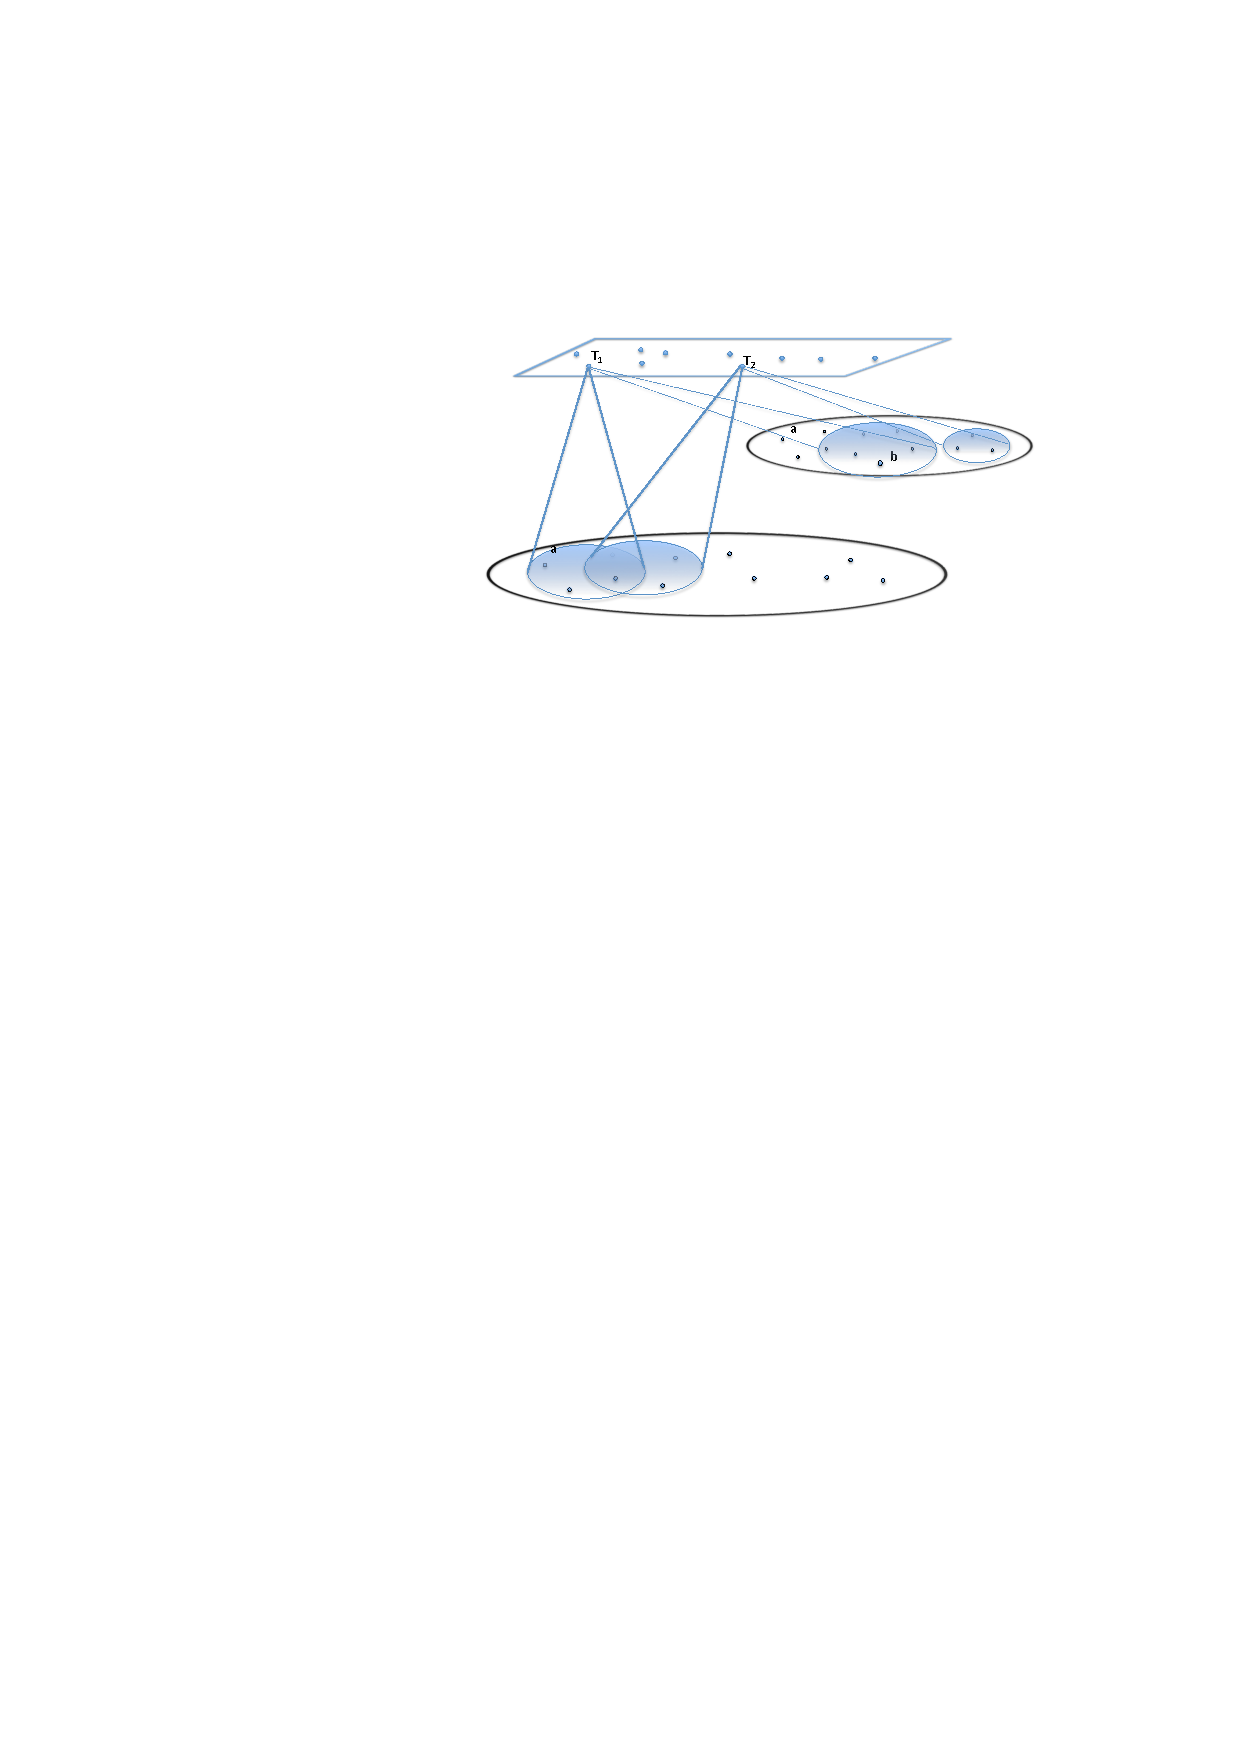
\includegraphics[width=\textwidth]{modal}
\begin{adjustbox}{max width=\textwidth}
\begin{tikzpicture}[
  type/.style={circle, inner sep=0pt, minimum size=6pt, ball color=BTypeCol},
  firsttype/.style={circle, inner sep=0pt, minimum size=6pt, ball color=FirstTypeCol},
  secondtype/.style={circle, inner sep=0pt, minimum size=6pt, ball color=SecondTypeCol},
  objects/.style={circle, inner sep=0pt, minimum size=6pt, ball color=ObjectCol},
  modalobjects/.style={circle, inner sep=0pt, minimum size=6pt, ball color=ModalCol}
  ]

  % basic types:
  \begin{scope}[
    % every node/.append style={yslant=0,xslant=1.75},
    yslant=0,xslant=1.75
    ]
    \filldraw [fill=BTypeCol, draw=BorderCol, thick, fill opacity=0.5] (0,0) rectangle (8,2);

    \foreach \x/\y in {0.5/1.3, 1.4/1.6, 1.8/1.3, 1.9/0.5, 3.3/1.8, 2.6/1.5, 4.4/0.9, 4.7/1, 5.5/0.3, 5.6/1.1, 5.5/1.7, 6.4/1.2, 6.7/1.6} {
      \node [type] at (\x,\y) {};
    }

    \node [coordinate] (btypeleft) at (0,1) {};
    \node [coordinate] (btyperight) at (8,1) {};

    \node [type, label=above:$T_1$] (t1) at (1.3,0.6) {};
    \node [type, label=above:$T_2$] (t2) at (4.5,0.5) {};
  \end{scope}    


  % objects:
  \begin{scope}[
    % every node/.append style={yslant=0,xslant=1.75},
    %yslant=0,xslant=1.75,
    yshift=-100
    ]
    \filldraw [fill=ObjectCol, opacity=0.4, draw=BorderCol, ultra thick] (5,0) ellipse (6 and 1);

    \foreach \a/\b in {5.5/0.7, 6.4/0.2, 6.7/0.6, 7/0, 7.5/0.35, 8/-0.3, 8.1/0.2, 8.7/0, 9/0.2, 10/0.1} {
      \node [objects] at (\a,\b) {};
    }
    % for T1 from BType:
    \node [modalobjects, label=above:$a$] (o1) at (0.3,-0.1) {}; 
    \node [objects] (o2) at (1,0.35) {}; 
    \node [objects] (o3) at (1.6,-0.2) {};
    \node [ellipse, fit=(o1) (o2) (o3), yscale=0.7, draw=BTypeCol, thick, fill=BTypeCol, fill opacity=0.3] (fitA) {};
    \draw [BTypeCol, thick] (t1) -- (fitA.east);
    \draw [BTypeCol, thick] (t1) -- (fitA.west);

    % for T2 from BType:
    \node [objects] (o4) at (2.6,-0.5) {};
    \node [objects] (o5) at (3.1,-0.5) {};
    \node [objects] (o6) at (3.3,-0.1) {};
    \node [ellipse, fit=(o3) (o4) (o5) (o6), yscale=0.7, draw=BTypeCol, thick, fill=BTypeCol, fill opacity=0.2] (fitB) {};
    \draw [BTypeCol, thick] (t2) -- (fitB.east);
    \draw [BTypeCol, thick] (t2) -- (fitB.west);

    % % for T2 from Type1:
     \node [objects] (o7) at (4,0.4) {};
     \node [objects] (o8) at (4.4,0) {}; 
     \node [objects] (o9) at (4.7,0.1) {};
    % \node [ellipse, fit=(o3) (o4) (o5) (o6) (o7) (o8) (o9), yscale=0.6, xscale=0.9, draw=FirstTypeCol, thick, fill=FirstTypeCol, fill opacity=0.2] (fitC) {};

    % % for T2 from Type2:
     \node [objects] (o10) at (5.5,-0.3) {};
     \node [objects] (o11) at (5.6,-0.1) {};
    % \node [ellipse, fit=(o3) (o4) (o5) (o6) (o7) (o8) (o9) (o10) (o11), yscale=0.7, xscale=0.8, draw=SecondTypeCol, thick, fill=SecondTypeCol, fill opacity=0.2] (fitD) {};
  \end{scope}


  % modal types:
  \begin{scope}[
    % every node/.append style={yslant=0,xslant=1.75},
    %yslant=0,xslant=1.75,
    yshift=-35, 
    xshift=220
    ]
    \filldraw [fill=ObjectCol, opacity=0.4, draw=BorderCol, ultra thick] (3.5,0) ellipse (4 and 0.75);

    \foreach \a/\b in {0.3/-0.1, 1.5/-0.3, 3.9/0.2, 7/0} {
      \node [objects] at (\a,\b) {};
    }
    \node [modalobjects, label=above:$a$] at (0.7,0) {};
    \node [objects] (i1) at (5.7,-0.2) {};
    \node [objects] (i2) at (6.1,0.3) {};
    \node [objects] (i3) at (5,0) {};
    \node [ellipse, fit=(i1) (i2) (i3), yscale=0.7, draw=BTypeCol,
    thick, fill=BTypeCol, fill opacity=0.2] (fitAA) {};
    \draw [BTypeCol, thick] (t2) -- (fitAA.north);
    \draw [BTypeCol, thick] (t2) -- (fitAA.south west);

    \node [objects] (i4) at (1.6,0.1) {};
    \node [objects] (i5) at (2,0.2) {};
    \node [modalobjects, label=above:$b$] (i6) at (2.5,-0.3) {};
    \node [objects] (i7) at (2.7,0.35) {};
    \node [ellipse, fit=(i4) (i5) (i6) (i7), yscale=0.7, xscale=1.1,
    draw=BTypeCol, thick, fill=BTypeCol, fill opacity=0.2] (fitBB) {};
    \draw [BTypeCol, thick] (t1) -- (fitBB.north);
    \draw [BTypeCol, thick] (t1) -- (fitBB.south west);
  \end{scope}


  % % Type1:
  % \begin{scope}[
  %   % every node/.append style={yslant=0,xslant=1.75},
  %   yslant=0,xslant=1.75,
  %   xshift=-100,
  %   yshift=80
  %   ]
  %   \filldraw [fill=FirstTypeCol, draw=BorderCol, thick, fill opacity=0.3] (0,0) rectangle (8,2);
  %   \node [coordinate] (firsttypeleft) at (0,1) {};
  %   \node [coordinate] (firsttyperight) at (8,1) {};

  %   \foreach \x/\y in {0.45/1.4, 1.4/1.6, 1.9/0.5, 3.3/1.8, 2.6/1.5, 4.7/1, 5.5/0.3, 5.6/1.1,  6.7/1.6} {
  %     \node [firsttype] at (\x,\y) {};
  %   }

  %   \node [firsttype, label=above:$T_1$] (ft1) at (1.8,1.1) {};
  %   \node [firsttype, label=above:$T_2$] (ft2) at (5.8,0.7) {};
  %   \node [firsttype, label=above:$T_3$] (ft3) at (6.4,1.2) {};
  %   \node [firsttype, label=above:{\textbf{Type$^1$}}] (ft) at (4,0.4) {};

  %   \draw [FirstTypeCol, thick] (ft) -- (btypeleft);
  %   \draw [FirstTypeCol, thick] (ft) -- (btyperight);
    
  %   \draw [FirstTypeCol, thick] (ft2) -- (fitC.east);
  %   \draw [FirstTypeCol, thick] (ft2) -- (fitC.west);
  % \end{scope}    


  % % Type2:
  % \begin{scope}[
  %   % every node/.append style={yslant=0,xslant=1.75},
  %   yslant=0,xslant=1.75,
  %   xshift=-200,
  %   yshift=160
  %   ]
  %   \filldraw [fill=SecondTypeCol, draw=BorderCol, thick, fill opacity=0.1] (0,0) rectangle (8,2);
  %   \foreach \x/\y in {1.4/1.6, 1.9/0.5, 3.2/1.5, 4.7/1, 5.4/1.2, 5.8/0.3, 6/0.3,  6.2/1.6} {
  %     \node [secondtype] at (\x,\y) {};
  %   }

  %   \node [secondtype, label=above:$T_1$] (st1) at (1.2,1) {};
  %   \node [secondtype, label=above:$T_2$] (st2) at (4.8,0.7) {};
  %   \node [secondtype, label=above:$T_3$] (st3) at (2.6,1.3) {};
  %   \node [secondtype, label=above:{\textbf{Type$^2$}}] (st) at (3.4,0.5) {};

  %   \draw [SecondTypeCol, thick] (st) -- (firsttypeleft);
  %   \draw [SecondTypeCol, thick] (st) -- (firsttyperight);
    
  %   \draw [SecondTypeCol, thick] (st2) -- (fitD.east);
  %   \draw [SecondTypeCol, thick] (st2) -- (fitD.west);
  % \end{scope}    
\end{tikzpicture}
\end{adjustbox}

\caption{Modal system of basic types}
\label{fig:modal}
\end{figure}
The object $a$ is
of type $T_1$ in the first possibility but not in the second
possibility.  There is an object, $b$, of type $T_1$ in the second
possibility.  $b$ does not exist at all in the first possibility.
In the
figure we just show two possibilities but our general definition in
Appendix~\ref{app:modal}, introduced in Chapter~\ref{ch:percint}, p.~\pageref{ex:modalsys-complex},
allows for there to be any number of possibilities, including
infinitely many.

% \begin{shaded}

% We start by characterizing a modal system of basic types in \nexteg{},
% repeated in Appendix~\ref{sec:basic}.
% \begin{ex} 
 

% A \textit{modal system of basic types} is a family of
% pairs:
% \begin{display}
% \textbf{TYPE$_{\mathit{MB}}$} = $\langle${\bf Type},
% $A\rangle_{A\in\mathcal{A}}$
% \end{display}
% where:
% \begin{enumerate} 
 
% \item $\mathcal{A}$ is a set of functions with domain \textbf{Type} 
 
% \item for each $A\in\mathcal{A}$, $\langle${\bf Type}, $A\rangle$ is a
%   system of basic types
 
% \end{enumerate}
% \label{ex:def-modal-basic-types}
% \end{ex} 
  
% \end{shaded}


Given this apparatus we define four simple modal notions:
\begin{description}

\item[(necessary) equivalence] Two types are (necessarily) equivalent
  just in case the extension of one type is identical with that of
  the other type in all the possibilities.  While the different
  possibilities may provide different extensions for the types, it
  will always be the case that in any given possibility the two types
  will have the same extension.

\item[subtype] One type is a subtype of another just in case whatever
  possibility you look at it is always the case that the extension of
  the first type is a subset of the extension of the second.  We can
  also say that the first type ``entails'' the second, that is, any
  object which is of the first type will also be of the second type,
  no matter which possibility you are considering.

\item[necessity] The notion of necessity we characterize for a type
  could be glossed as ``necessarily realized'' or ``necessarily
  instantiated''.  A type will be necessary just in case there is
  something of the type in all the possibilities.

\item[possibility] This notion corresponds to ``possibly realized'' or
  ``possibly instantiated''.  A type will be possible just in case
  there is some possibility according to which it has a non-null
  extension.

\end{description}

\begin{shaded}

These notions are made precise for modal systems of complex types in
\nexteg{} and (\ref{ex:inclusive-modal-notions}), repeated in Appendix~\ref{app:modal}.  As a preliminary we
note that if
\begin{quote}
{\bf TYPE$_{\mathit{MC}}$} = $\langle${\bf Type}$_M$, {\bf BType},
$\langle$\textbf{PType}$_M$, {\bf Pred}, \textbf{ArgIndices}, {\it
  Arity\/}$\rangle, M\rangle_{M\in\mathcal{M}}$
\end{quote}
is a modal system of complex types based
on $\mathcal{M}$, we shall use the notation {\bf
  TYPE$_{\mathit{MC}_M}$} (where $M\in\mathcal{M}$) to refer to that
system of complex types in {\bf TYPE$_{\mathit{MC}}$} whose model is
$M$.  Let \textbf{Type}$_{\mathit{MC}_{\mathit{restr}}}$ be
  $\bigcap\limits_{M\in\mathcal{M}}\!\textbf{Type}_M$, the
  ``restrictive'' set of
  types which occur in all possibilities,  and \textbf{Type}$_{\mathit{MC}_{\mathit{incl}}}$ be
  $\bigcup\limits_{M\in\mathcal{M}}\!\textbf{Type}_M$, the
  ``inclusive'' set of
  types which occur in at least one possibility. Then we can define
  modal notions either restrictively or inclusively (indicated by the
  subscripts $r$ and $i$ respectively).

 \begin{ex} 
\textbf{restrictive modal notions}  
\begin{subex} 
 
\item for any $T_1,T_2\in\textbf{Type}_{\mathit{MC}_{\mathit{restr}}}$, $T_1$ \textit{is
    (necessarily) equivalent$_r$
    to} $T_2$ \textit{in} {\bf TYPE$_{\mathit{MC}}$},
  $T_1\approx_{\mathbf{TYPE_{\mathit{MC}}}}T_2$,  iff for all
  $M\in\mathcal{M}$, $\{a\mid a:_{\mathbf{TYPE}_{\mathit{MC}_M}}T_1\}=\{a\mid a:_{\mathbf{TYPE}_{\mathit{MC}_M}}T_2\}$
  
 
\item for any $T_1,T_2\in\textbf{Type}_{\mathit{MC}_{\mathit{restr}}}$, $T_1$ \textit{is a subtype$_r$ of} $T_2$ \textit{in} {\bf TYPE$_{\mathit{MC}}$},
  $T_1\sqsubseteq_{\mathbf{TYPE_{\mathit{MC}}}}T_2$,  iff for all
  $M\in\mathcal{M}$, $\{a\mid a:_{\mathbf{TYPE}_{\mathit{MC}_M}}T_1\}\subseteq\{a\mid a:_{\mathbf{TYPE}_{\mathit{MC}_M}}T_2\}$

\item for any $T\in\textbf{Type}_{\mathit{MC}_{\mathit{restr}}}$, $T$ \textit{is necessary$_r$ in} {\bf TYPE$_{\mathit{MC}}$}  iff for all
  $M\in\mathcal{M}$, \\ $\{a\mid a:_{\mathbf{TYPE}_{\mathit{MC}_M}}T\}\not=\emptyset$

\item for any $T\in\textbf{Type}_{\mathit{MC}_{\mathit{restr}}}$, $T$ \textit{is possible$_r$ in} {\bf TYPE$_{\mathit{MC}}$}  iff for some
  $M\in\mathcal{M}$, \\ $\{a\mid a:_{\mathbf{TYPE}_{\mathit{MC}_M}}T\}\not=\emptyset$
 
\end{subex}

\end{ex}

\begin{ex}
\textbf{inclusive modal notions}
\begin{subex} 
 
\item for any $T_1,T_2\in\textbf{Type}_{\mathit{MC}_{\mathit{incl}}}$, $T_1$ \textit{is
    (necessarily) equivalent$_i$
    to} $T_2$ \textit{in} {\bf TYPE$_{\mathit{MC}}$},
  $T_1\approx_{\mathbf{TYPE_{\mathit{MC}}}}T_2$,  iff for all
  $M\in\mathcal{M}$, if $T_1$ and $T_2$ are members of
  \textbf{Type}$_M$, then $\{a\mid a:_{\mathbf{TYPE}_{\mathit{MC}_M}}T_1\}=\{a\mid a:_{\mathbf{TYPE}_{\mathit{MC}_M}}T_2\}$
  
 
\item for any $T_1,T_2\in\textbf{Type}_{\mathit{MC}_{\mathit{incl}}}$, $T_1$ \textit{is a subtype$_i$ of} $T_2$ \textit{in} {\bf TYPE$_{\mathit{MC}}$},
  $T_1\sqsubseteq_{\mathbf{TYPE_{\mathit{MC}}}}T_2$,  iff for all
  $M\in\mathcal{M}$, if $T_1$ and $T_2$ are members of
  \textbf{Type}$_M$, then $\{a\mid a:_{\mathbf{TYPE}_{\mathit{MC}_M}}T_1\}\subseteq\{a\mid a:_{\mathbf{TYPE}_{\mathit{MC}_M}}T_2\}$

\item for any $T\in\textbf{Type}_{\mathit{MC}_{\mathit{incl}}}$, $T$ \textit{is necessary$_i$ in} {\bf TYPE$_{\mathit{MC}}$}  iff for all
  $M\in\mathcal{M}$, if $T\in$\textbf{Type}$_M$, then \\ $\{a\mid a:_{\mathbf{TYPE}_{\mathit{MC}_M}}T\}\not=\emptyset$

\item for any $T\in\textbf{Type}_{\mathit{MC}_{\mathit{incl}}}$, $T$ \textit{is possible$_i$ in} {\bf TYPE$_{\mathit{MC}}$}  iff for some
  $M\in\mathcal{M}$, if $T\in$\textbf{Type}$_M$, then\\ $\{a\mid a:_{\mathbf{TYPE}_{\mathit{MC}_M}}T\}\not=\emptyset$
 
\end{subex} 
\label{ex:inclusive-modal-notions}
\end{ex} 

It is easy to see that if any of the restrictive definitions holds for
given types in a particular system then the corresponding inclusive
definition will also hold for those types in that system.

This can be recast in terms of our informal proof theoretic notation
where we use `$T\ \mathrm{true}$' to represent that $T$ has some
witness, `$T_1\sqsubseteq_rT_2$' (`$T_1\sqsubseteq_iT_2$') to
represent that $T_1$ is a restrictive (inclusive) subtype of $T_2$,
`$T_1\approx_rT_2$' (`$T_1\approx_iT_2$') to represent that $T_1$ is
restrictively (inclusively) equivalent to $T_2$, `$T\ \mathrm{nec}_r$'
(`$T\ \mathrm{nec}_i$') to represent that $T$ is restrictively
(inclusively) necessary and `$T\ \mathrm{poss}_r$' (`$T\
\mathrm{poss}_i$') to represent that $T$ is restrictively
(inclusively) possible.  We give the restrictive notions in \nexteg{}.
\begin{ex} 
  \textbf{restrictive modal notions}

  For $\mathcal{G}$ a modal system of complex types
  \begin{subex} 
 
  \item
    \begin{prooftree}
      \hypo{[\Gamma\in\mathcal{G}]}
      \ellipsis{}{\Gamma\vdash T_1\in\textbf{Type}}
      \hypo{[\Gamma\in\mathcal{G}]}
      \ellipsis{}{\Gamma\vdash T_2\in\textbf{Type}}
      \hypo{[\Gamma\in\mathcal{G},\Gamma\vdash a:T_1]}
      \ellipsis{}{\Gamma\vdash a:T_2}
      \infer3{\mathcal{G}\vdash T_1\sqsubseteq_r T_2}
    \end{prooftree}
    
 
  \item
    \begin{prooftree}
      \hypo{\mathcal{G}\vdash T_1\sqsubseteq_r T_2}
      \hypo{\mathcal{G}\vdash T_2\sqsubseteq_r T_1}
      \infer2{\mathcal{G}\vdash T_1\approx_r T_2}
    \end{prooftree}

    
  \item
    \begin{prooftree}
      \hypo{[\Gamma\in\mathcal{G}]}
      \ellipsis{}{\Gamma\vdash T\in\textbf{Type}}
      \hypo{[\Gamma\in\mathcal{G}]}
      \ellipsis{}{\Gamma\vdash T\ \mathrm{true}}
      \infer2{\mathcal{G}\vdash T\ \mathrm{nec}_r}
    \end{prooftree}

    
  \item
    \begin{prooftree}
      \hypo{[\Gamma\in\mathcal{G}]}
      \ellipsis{}{\Gamma\vdash T\in\textbf{Type}}
      \hypo{\Gamma'\in\mathcal{G}}
      \hypo{\Gamma'\vdash a:T}
      \infer3{\mathcal{G}\vdash T\ \mathrm{poss}_r}
    \end{prooftree}
    
 
\end{subex} 
  
\end{ex}
The inclusive notions are given in \nexteg{}.
\begin{ex} 
  \textbf{inclusive modal notions}

  For $\mathcal{G}$ a modal system of complex types
  \begin{subex} 
 
  \item
    \begin{prooftree}
      \hypo{[\Gamma\in\mathcal{G},\Gamma\vdash
        T_1\in\textbf{Type},\Gamma\vdash
        T_2\in\textbf{Type},\Gamma\vdash a:T_1]}
      \ellipsis{}{\Gamma\vdash a:T_2}
      \infer1{\mathcal{G}\vdash T_1\sqsubseteq_i T_2}
    \end{prooftree}
    
 
  \item
    \begin{prooftree}
      \hypo{\mathcal{G}\vdash T_1\sqsubseteq_i T_2}
      \hypo{\mathcal{G}\vdash T_2\sqsubseteq_i T_2}
      \infer2{\mathcal{G}\vdash T_1\approx_i T_2}
    \end{prooftree}

    
  \item
    \begin{prooftree}
      \hypo{\Gamma'\in\mathcal{G}}
      \hypo{\Gamma'\vdash T\in\textbf{Type}}
      \hypo{[\Gamma\in\mathcal{G},\Gamma\vdash T\in\textbf{Type}]}
      \ellipsis{}{\Gamma\vdash T\ \mathrm{true}}
      \infer3{\mathcal{G}\vdash T\ \mathrm{nec}_i}
    \end{prooftree}

    
  \item
    \begin{prooftree}
      \hypo{\Gamma\in\mathcal{G}}
      \hypo{\Gamma\vdash T\in\textbf{Type}}
      \hypo{\Gamma\vdash a:T}
      \infer3{\mathcal{G}\vdash T\ \mathrm{poss}_i}
    \end{prooftree}
    
    
 
\end{subex} 
  
\end{ex} 
  
  





\end{shaded}



Note that
all of these notions are relativized to the modal system you are
considering and the possibilities it offers.  We may think of the
family of assignments $\mathcal{A}$ as providing a modal base in the
sense of \cite{Kratzer2012}.
We may wish to consider very small families of
assignments corresponding to the knowledge we have.  Alternatively, we
may want to consider strong logical variants of these modal notions
where we consider all the logical possibilities, for example, all
possible assignments of extensions to types.

% So far we have talked about modal systems of basic types.  Modal
% systems of complex types, where we introduce ptypes, create a
% minor complication.  What ptypes that are present in a system depends
% on what objects there are of the types that are used in the arities of
% the predicates.  Thus if we have some predicate $r$ with arity
% $\langle\textit{Ind},\textit{Ind}\rangle$ and a possibility where the
% set assigned to \textit{Ind} is $\{a,b\}$ then according to that
% possibility the ptypes formed with $r$ will be $r(a,a)$, $r(a,b)$,
% $r(b,a)$ and $r(b,b)$.  In a possibility where \textit{Ind} is
% assigned a different set the set of available ptypes will be
% different.  It is an important feature of type theories with types
% constructed from predicates that the collection of such types depends
% on what objects are available as arguments to the predicates.  This
% makes type theory very different from a logical language such as
% predicate calculus where the notion of well-formedness of syntactic
% expressions containing predicates is defined independently of what is
% provided by the model as denotations of arguments to the predicate.

% This leads us (in Appendix~\ref{app:modal}) to define two variants of
% each of our modal notions: \textit{restrictive} variants which are only defined
% for types which exist in all possibilities and \textit{inclusive}
% variants which require that the modal definition holds for all the
% possibilities in which the types exist and disregards those in which
% the types do not exist.  For example, a type is \textit{necessary}$_r$
% (that is, ``restrictively necessary'') just in case the type is
% available in all possibilities and has a non-empty set of witnesses in
% all possibilities.  It is \textit{necessary}$_i$ (``inclusively
% necessary'') just in case in all the possibilities in which the type
% is provided it has a non-empty set of witnesses.  It is clear that if
% a type is necessary$_r$ it will also be necessary$_i$ but there may be
% types which are necessary$_i$ but not necessary$_r$ (if the type is
% not provided in all possibilities).  A similar relationship between
% the restrictive and inclusive notions holds for all the modal notions
% we have discussed.

% There may be significant classes of modal type systems in which the
% types available in the different possibilities do not vary.  This
% could be achieved by requiring that the types used in the arities of
% predicates always have the same witnesses in all the possibilities.
% This seems feasible if we restrict the types used in predicate arities
% to basic ontological categories such as individual or time point.  It
% seems reasonable to consider modal systems in which an individual in
% one possibility will be an individual in any other possibility, for
% example.  It seems reasonable to say that we wish to consider
% possibilities where, for example, Kim is a man rather than a woman,
% but not possibilities where Kim is a point in time rather than an
% individual.  However, the notion ``basic ontological category'' is a
% slippery one and we do not want to be forced to make commitments about that.

% In the definition of a system of complex types in
% section~\ref{app:comptypes}  we call the pair of an assignment to
% basic types and assignment to ptypes, $\langle A,F\rangle$, a \textit{model} because of its
% similarity to first order models.\footnote{For a more detailed
%   discussion of the relationship between this and first order models
%   as used in the interpretation of first order logic see
%   \cite{Cooperforthcoming}.} The model provides an interface
% between 
% the type theoretical system and a domain external to the type theory.
% The natural domain to relate to the type theory is that of individuals
% and situations, that is the kind of things we can perceive or at least
% consider as possibilities.  However, we may want to use models which
% relate to our perceptual apparatus, as in \cite{Larsson2011}, rather
% than directly to the world.  This can also be the key for relating the
% type theory to a dynamically changing world where the models
% representing our perceived possibilities are not fixed.  % We will
% return to this in Chapter~\ref{ch:coord}.





\section{Modality without possible worlds}

\cite{Montague1973} introduces \textit{necessarily} and
\textit{possibly} as sentence adverbs, that is, they combine with a
sentence to produce another sentence. If $\alpha$ is a sentence, then
\textit{necessarily} $\alpha$ is true in a possible world, $w$, just in case $\alpha$ is true in
every possible world and \textit{possibly} $\alpha$ is true in a
possible world, $w$, just in case there is some possible world in
which $\alpha$ is true.\footnote{This simple treatment of modality
  corresponds to the modal logic system S5 where there is no
  restriction on accessibility between possible worlds
  \citep{HughesCresswel1968,HughesCresswell1996}.}

In Chapter~\ref{ch:percint}, p.~\pageref{pg:modal-systems} and
Appendix~\ref{app:modal} we introduce modal type systems which are
families of type systems, which we call \textit{possibilities}, differing in their assignments of
witnesses to basic types and ptypes.  The important difference between
possible worlds and possibilities is that for possibilities the
parameters along which they can vary are fixed by the available types
introduced in the type system, a well-defined notion, and one which
varies depending on the particular type system.  Thus we have a way of
characterizing the dimensions along which the possibilities associated
with a given type system vary and thus we have a way of representing the
possibilities, whereas we do not have such a way of characterizing
possible worlds.  Building on the modal notions that we introduced in
Section~\ref{sec:percint-modal} we can introduce type constructors `$\Box$' and `$\Diamond$' corresponding to the operators in modal
logic as
in \nexteg{}.
\begin{ex} 
If $T$ is a type, then $\Box_r T$, $\Box_i T$, $\Diamond_r T$ and $\Diamond_i T$ are types 
\end{ex}



These types obey the constraints in \nexteg{} which correspond to the
truth conditions for the corresponding operators in modal logic (S5).
\begin{ex} 
\begin{subex} 
 
\item $\Box_{r/i} T$ is non-empty iff $T$ is restrictively/inclusively
  necessary (approximately, non-empty in all possibilities) 
 
\item $\Diamond_{r/i} T$ is non-empty iff $T$ is
  restrictively/inclusively possible (approximately, non-empty in some possibility) 
 
\end{subex} 
\label{ex:modalconds}   
\end{ex}

\begin{shaded}
Making the witness conditions for these types meet the constraints in
\preveg{} is a little tricky.  We do not have biconditionals, but two
conditionals which correspond to introduction and elimination rules in
proof theory.  Suppose that $\mathbb{T}$ is a modal type system and
that $p\in\mathbb{T}$ is a possibility in $\mathbb{T}$. Then for
`$\Box_{r\i} T$ we have \nexteg{}.
\begin{ex} 
\begin{subex} 
 
\item If $a:_p\Box_{r/i}T$ then $T$ is necessary$_{r/i}$ in $\mathbb{T}$ 
 
\item If $T$ is necessary$_{r/i}$ in $\mathbb{T}$ then for any
  $p'\in\mathbb{T}$ there is some $a'$ such that $a':_{p'}\Box_{r/i}T$  
 
\end{subex} 
\label{ex:witconds-Box}   
\end{ex} 
Note that the two clauses in \preveg{} jointly entail \nexteg{}.
\begin{ex} 
For any $p'\in\mathbb{T}$ there is some $a'$ such that
$a':_{p'}\Box_{r/i}T$ (``$\Box_{r/i}T$ is true in $p'$'') iff $T$ is
necessary$_{r/i}$ in $\mathbb{T}$ 
\end{ex} 
For `$\Diamond_{r/i}T$' we have \nexteg{}.
\begin{ex} 
\begin{subex} 
 
\item If $a:_p\Diamond_{r/i}T$ then $T$ is possible$_{r/i}$ in $\mathbb{T}$ 
 
\item If $T$ is possible$_{r/i}$ in $\mathbb{T}$ then for any $p'\in\mathbb{T}$ there is some $a'$ such that $a':_{p'}\Diamond_{r/i}T$ 
 
\end{subex}
\label{ex:witconds-Diamond}
   
\end{ex} 
The two clauses in \preveg{} jointly entail \nexteg{}.
\begin{ex} 
For any $p'\in\mathbb{T}$ there is some $a'$ such that
$a':_{p'}\Diamond_{r/i}T$ (``$\Diamond_{r/i}T$ is true in $p'$'') iff $T$ is
possible$_{r/i}$ in $\mathbb{T}$ 
\end{ex} 
We can recreate the witness conditions in (\ref{ex:witconds-Box}) and
(\ref{ex:witconds-Diamond}) in our informal proof theoretic
representation as in \nexteg{} where we use $\mathcal{G}\vdash T\text{
  nec/poss}_{r/i}$ to represent $T$ is necessary/possible$_{r/i}$ in $\mathcal{G}$.
\begin{ex}
  For $\mathcal{G}$ a modal system of complex types:
\begin{subex} 
 
\item
  \begin{prooftree}
    \hypo{\Gamma\in\mathcal{G}}
    \hypo{\Gamma\vdash a:\Box_{r/i} T}
    \infer2{\mathcal{G}\vdash T\text{ nec}_{r/i}}
  \end{prooftree}
  
 
\item
  \begin{prooftree}
    \hypo{\mathcal{G}\vdash T\text{ nec}_{r/i}}
    \hypo{\Gamma\in\mathcal{G}}
    \infer2{\Gamma\vdash\Box_{r/i}T\text{ true}}
  \end{prooftree}

  
\item
  \begin{prooftree}
    \hypo{\Gamma\in\mathcal{G}}
    \hypo{\Gamma\vdash a:\Diamond_{r/i} T}
    \infer2{\mathcal{G}\vdash T\text{ poss}_{r/i}}
  \end{prooftree}

  
\item
  \begin{prooftree}
    \hypo{\mathcal{G}\vdash T\text{ poss}_{r/i}}
    \hypo{\Gamma\in\mathcal{G}}
    \infer2{\Gamma\vdash\Diamond_{r/i}T\text{ true}}
  \end{prooftree}
  
 
\end{subex} 
   
\end{ex} 
  


\end{shaded}
This shows how we can, if we want to, recreate in TTR the simple S5 modal
system (that is, where all possibilities are accessible to each other)
that \cite{Montague1973} uses.

% In order to see how we can meet these constraints we have to first
% note that in a modal type system we cannot talk of an object $a$ being
% of a type $T$ \textit{tout court} as we have done so far.  $a$ may be
% of type $T$ in some possibilities but not others.  This means that we
% have to relativize being of a type to possibilities,
% $p$ which are members of a modal type system, $\mathcal{P}$. Instead of writing $a:T$, we will write $a:_{p,\mathcal{P}} T$ (``$a$ is of
% type $T$ in possibility $p$ within modal type system $\mathcal{P}$'').\footnote{Note that in Appendix~\ref{app:ttr} we have throughout
%   the formal development of TTR always relativized the of-type
%   relation to the type system being considered, and in the case of
%   modal type systems in addition to the possibility (identified by the
%   model associated with the possibility).} We also correspondingly
% relativize our notation for the set of witnesses of a type as in
% \nexteg{}.
% \begin{ex} 
% $\down{T}_{p,\mathcal{P}} = \{a\mid a:_{p,\mathcal{P}}T\}$ 
% \end{ex} 
% We introduce two basic types of types, \textit{Nec} and \textit{Poss},
% the types of necessary and possible propositions respectively.  The
% witness conditions for these types are given in
% \nexteg{}.\footnote{Note that it is important for these types that we
%   have introduced stratified types (Appendix~\ref{app:int}) since
%   \textit{Nec} and \textit{Poss} can themselves be necessary and
%   possible types. For example, instead of \textit{Nec}
%   :$_{p,\mathcal{P}}$ \textit{Nec} we have \mbox{\textit{Nec}$^n$
%   :$_{p,\mathcal{P}}$ \textit{Nec}$^{n+1}$} to avoid the danger of
%   running into a version of Russell's paradox.  As usual we will
%   suppress discussion of stratification in the text in order to
%   simplify the presentation.}
% \begin{ex} 
% \begin{subex} 
 
% \item $T:_{p,\mathcal{P}}$ \textit{Nec} iff for all
%   $p'\in\mathcal{P}$, $\down{T}_{p',\mathcal{P}}\not=\emptyset$ 
 
% \item $T:_{p,\mathcal{P}}$ \textit{Poss} iff for some
%   $p'\in\mathcal{P}$, $\down{T}_{p',\mathcal{P}}\not=\emptyset$  
 
% \end{subex} 
   
% \end{ex} 
% Now consider that the inclusion of singleton types in our system
% (Appendix~\ref{app:singletontypes}) allows for the types
% \textit{Nec}$_T$ and \textit{Poss}$_T$ for any type, $T$.  These types
% have a single witness, $T$, if $T$ is necessary or possible
% respectively and otherwise have no witnesses. These types thus meet
% the constraints on $\Box T$ and $\Diamond T$ given in
% (\ref{ex:modalconds}).  We propose therefore to make the
% identifications given in \nexteg{}.
% \begin{ex} 
% \begin{subex} 
 
% \item $\Box T = \textit{Nec}_T$ 
 
% \item $\Diamond T = \textit{Poss}_T$ 
 
% \end{subex} 
   
% \end{ex}

We have used the symbols `$\Box$' and `$\Diamond$' above to suggest
the relationship between our proposal in terms of types and the
traditional formulas of modal logic.  We could, however, have achieved
the same effect as above by introducing predicates `nec$_{r/i}$' and `poss$_{r/i}$'
with arity
$\langle$\textit{Type}$\rangle$ and giving ptypes of the form
`nec$_{r/i}(T)$' and `poss$_{r/i}(T)$' the same witness conditions as
above. % which obey the constraints in
% \nexteg{}.
% \begin{ex} 
% \begin{subex} 
% 
% \item $\down{\text{nec}(T)} \not=\emptyset$ iff $T$ : \textit{Nec} 
% 
% \item $\down{\text{poss}(T)} \not=\emptyset$ iff $T$ : \textit{Poss} 
% 
% \end{subex} 
%   
% \end{ex} 
We will pursue this option below where we will add additional arguments to the predicate.   
   
How many possibilities are there in a modal type system?  The answer
to this question is that there can be as many as you choose for the
given type system, ranging from a small finite number of possibilities
to a higher order infinity.  The definition of a modal type system
given in Appendix~\ref{app:modal} only requires that there be a family
of possibilities.  Thus this definition includes the kind of
restricted sets of ``possible worlds'' differing along a small finite
set of parameters which probability theorists talk of and indeed also
linguistic semanticists talk of informally when they are in pedagogical
explanatory mode (see, for example, \citealp{DowtyWallPeters1981} and
a lot of recent literature on inquisitive semantics such as
\citealp{GroenendijkRoelofsen2012}).  

It is important in a modal type system that the identity criteria for
the possibilities are determined by the types provided by the system.
Two possibilities are distinct only if they differ in the witnesses
associated with some basic type or ptype.  It is not possible to make
distinctions for which you do not have appropriate types available.
Thus the range of possibilities is limited by the types which are
available to classify objects.

This is not to say that we have eliminated all potential decidability
problems from modal type systems.  Of course, if the types that we use
to construct the system are not decidable it may not be possible to
decide on identity for possibilities.  Even if all the types are
guaranteed to be decidable, given an inifinite
set of possibilities there cannot be any general guarantee that we can
decide whether an arbitrary type is necessary or possible or not since
we cannot visit every possibility in a finite amount of time.  We can
only be sure if we have some general argument about the
possibilities which does not involve inspecting each possibility
individually.  But having a way of distinguishing between
possibilities which may in the limit be undecidable is better than not
having a way of distinguishing between possibilities, other than that
they are distinct members of a set.

The work on modality in natural language which has followed after
Montague's original work all points to a more restricted kind of
modality which involves arguing from some basic assumptions to a
conclusion rather than considering all logical possibilities.  This
view of modality in natural language has been put forward by Kratzer
in a body of work beginning with \cite{Kratzer1977}.  This and other
papers by Kratzer on modality are collected in revised and commented
form in \cite{Kratzer2012} and there is much other literature which
builds on Kratzer's ideas.  An excellent introduction to Kratzer's
work is given in Chapter~3 of \cite{Portner2009}.  The essential idea is that modals like
\textit{must} (corresponding to necessity) and \textit{can}
(corresponding to possibility) must be interpreted relative to a
``conversational background'' which in \cite{Kratzer1981} (Chapter~2
of \citealp{Kratzer2012}) is split into two components, a \textit{modal base} and an
\textit{ordering source}. The modal base is a set of
propositions\footnote{Actually, a function which determines a set of
  propositions for each possible world.} which characterize the
assumptions from which we are arguing. The ordering source is a set of
propositions\footnote{Again relativized to possible worlds.} which determine an ideal which we are trying to get as
close to as possible.  It is called an ordering source because
Kratzer, following \cite{Lewis1981}, thinks of it as inducing a
partial ordering on possible worlds, in terms of their closeness to
the ideal. Kratzer's insight is that necessity and possibility in
natural language should be defined relative to a modal base and an
ordering source.  In simple terms, a proposition, $p$, is necessary with
respect to a modal base, $b$, and an ordering source (ideal), $i$,
just in case $p$
follows from the conjunction of $b$ and $i$.  A proposition, $p$, is
possible with respect to $b$ and $i$ just in case $p$ is consistent
with the conjunction of $b$ and $i$.

We shall construe Kratzer's propositions as types and we shall take
modal bases and ideals to be types as well.  To recreate a Kratzerian
semantics for necessity and possibility we let the predicates `nec'
and `poss' have arity $\langle$\textit{Type}, \textit{Type},
\textit{Type}$\rangle$.
\begin{shaded}
 % A predicate like `believe' which represents that an individual has an
% attitude (of belief) to a certain type should thus have an arity which
% requires its arguments to be an individual and a type.  That is, we
% should be able to construct the type believe($c$, hug($a$,$b$))
% corresponding to \textit{$c$ believes that $a$ hugs $b$}. 
In order to allow types constructed with these predicates we need to
create intensional modal type systems in addition to the intensional
type systems we introduced in Chapter~\ref{ch:percint},
p.~\pageref{ex:int-type-sys}.  An intensional modal system of complex
types is a family of intensional type systems each of which represents
a possibility. % This
% is made precise in Appendix~\ref{app:int}.  For more detailed
% discussion see \cite{Cooperforthcoming}.
Figure~\ref{fig:intensionalmodal} represents an intensional modal type
system where we indicate just the initial
three orders of an infinite hierarchy of type orders on just one of
the possibilities.  Let $M$ be a model, $\langle A,F\rangle$, where
$A$ is an assignment to basic types and $F$ an assignment to ptypes as
usual.  Let $\mathcal{M}$ be an infinite sequence of models, $M$, indexed by
the natural numbers, corresponding to the models for the type systems
of each order in an intensional type system.  We use $\mathcal{M}_n$
to represent the model for the $n$-th order in an intensional type
system.  We use $\mathfrak{M}$ to represent a set of such model
sequences, representing the model sequences for each of the
possibilities in the intensional modal type system.  We characterize
an intensional modal system of complex types in \nexteg{}, repeated in
Appendix~\ref{app:int}.
\begin{ex} 
 An {\it intensional modal system of complex types based on $\mathfrak{M}$\/} is a family,
indexed by the natural numbers, of families of quadruples indexed by
members of $\mathfrak{M}$:
\begin{display}
{\bf TYPE$_\mathit{IMC}$} = $\langle${\bf Type}$^n$, {\bf BType},
$\langle$\textbf{PType}$^n$, {\bf Pred}, \textbf{ArgIndices}, {\it
  Arity\/}$\rangle$, $\mathscr{M}_n$$\rangle_{\mathscr{M}\in\mathfrak{M},n\in\mathit{Nat}}$
\end{display}
where:
\begin{enumerate} 
 
\item for each $n$, $\langle${\bf Type}$^n$, {\bf BType},
$\langle$\textbf{PType}$^n$, {\bf Pred}, \textbf{ArgIndices}, {\it
  Arity\/}$\rangle$, $\mathscr{M}_n$$\rangle_{\mathscr{M}\in\mathfrak{M}}$ is a modal
  system of complex types based on $\{\mathscr{M}_n\mid \mathscr{M}\in\mathfrak{M}\}$ 
 
\item for each $\mathscr{M}\in\mathfrak{M}$, $\langle${\bf Type}$^n$, {\bf BType},
$\langle$\textbf{PType}$^n$, {\bf Pred}, \textbf{ArgIndices}, {\it
  Arity\/}$\rangle$, $\mathscr{M}_n$$\rangle_{n\in\mathit{Nat}}$ is an
  intensional system of complex types
 
\end{enumerate}
\label{ex:intensional-modal-type-sys}
\end{ex}

In terms of our informal proof theoretic notation we can say that if
we have an intensional modal type system $\mathbb{G}$, if
$\{\Gamma^n\}_{n\in\textit{Nat}}\in\mathbb{G}$ then $\{\Gamma^n\}_{n\in\textit{Nat}}$ obeys the rules for
intensional systems of types and if for some $m\in\textit{Nat}$,
$\mathcal{G}=\{\Gamma^m\mid\text{for some } X\in\mathbb{G}, \Gamma^m\in X\}$,
then $\mathcal{G}$ obeys the rules for modal systems of types.
  
\end{shaded}
\begin{figure}[h]
%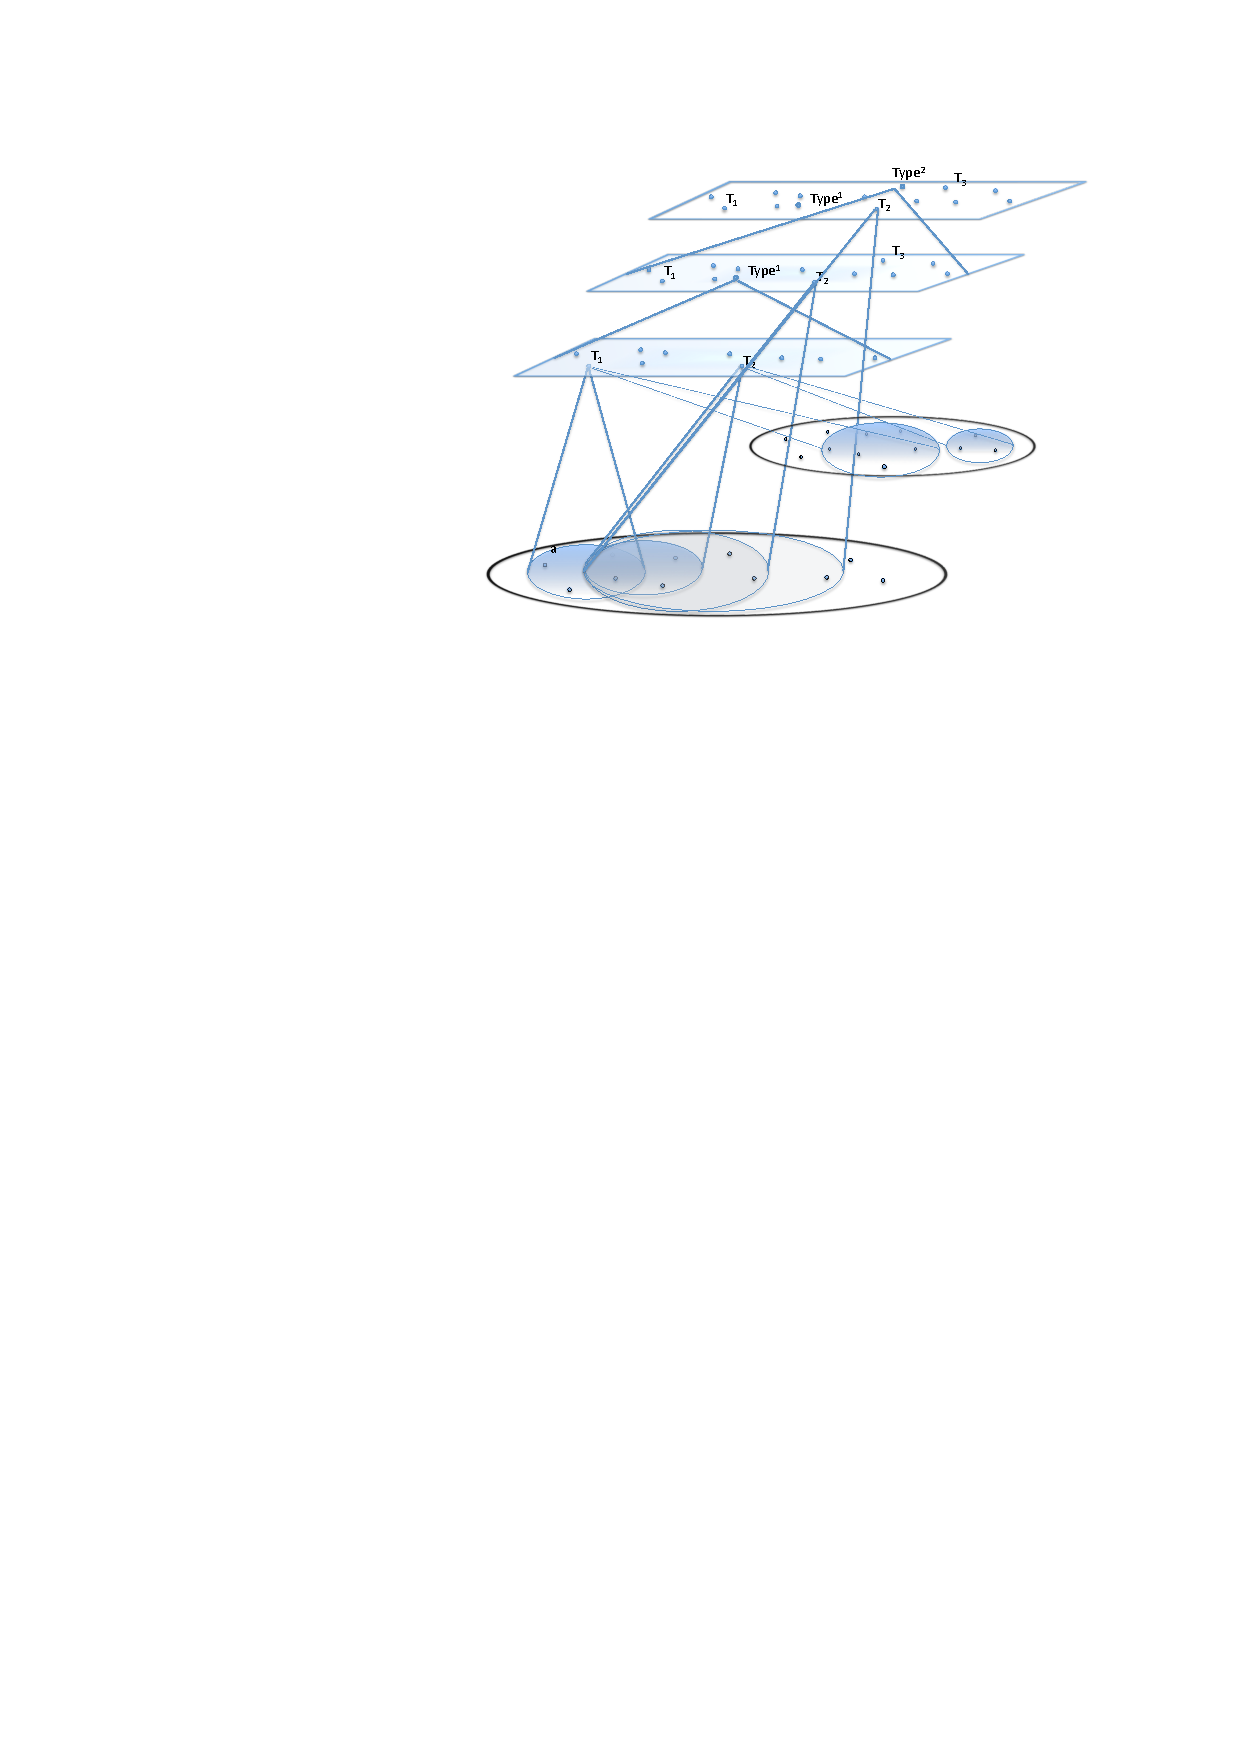
\includegraphics[width=\textwidth]{intensionalmodal}
\begin{adjustbox}{max width=\textwidth}
\begin{tikzpicture}[
  type/.style={circle, inner sep=0pt, minimum size=6pt, ball color=BTypeCol},
  firsttype/.style={circle, inner sep=0pt, minimum size=6pt, ball color=FirstTypeCol},
  secondtype/.style={circle, inner sep=0pt, minimum size=6pt, ball color=SecondTypeCol},
  objects/.style={circle, inner sep=0pt, minimum size=6pt, ball color=ObjectCol},
  modalobjects/.style={circle, inner sep=0pt, minimum size=6pt, ball color=ModalCol}
  ]

  % basic types:
  \begin{scope}[
    % every node/.append style={yslant=0,xslant=1.75},
    yslant=0,xslant=1.75
    ]
    \filldraw [fill=BTypeCol, draw=BorderCol, thick, fill opacity=0.5] (0,0) rectangle (8,2);

    \foreach \x/\y in {0.5/1.3, 1.4/1.6, 1.8/1.3, 1.9/0.5, 3.3/1.8, 2.6/1.5, 4.4/0.9, 4.7/1, 5.5/0.3, 5.6/1.1, 5.5/1.7, 6.4/1.2, 6.7/1.6} {
      \node [type] at (\x,\y) {};
    }

    \node [coordinate] (btypeleft) at (0,1) {};
    \node [coordinate] (btyperight) at (8,1) {};

    \node [type, label=above:$T_1$] (t1) at (1.3,0.6) {};
    \node [type, label=above:$T_2$] (t2) at (4.5,0.5) {};
  \end{scope}    


  % objects:
  \begin{scope}[
    % every node/.append style={yslant=0,xslant=1.75},
    %yslant=0,xslant=1.75,
    yshift=-100
    ]
    \filldraw [fill=ObjectCol, opacity=0.4, draw=BorderCol, ultra thick] (5,0) ellipse (6 and 1);

    \foreach \a/\b in {5.5/0.7, 6.4/0.2, 6.7/0.6, 7/0, 7.5/0.35, 8/-0.3, 8.1/0.2, 8.7/0, 9/0.2, 10/0.1} {
      \node [objects] at (\a,\b) {};
    }
    % for T1 from BType:
    \node [objects] (o1) at (0.3,-0.1) {}; 
    \node [objects] (o2) at (1,0.35) {}; 
    \node [objects] (o3) at (1.6,-0.2) {};
    \node [ellipse, fit=(o1) (o2) (o3), yscale=0.7, draw=BTypeCol, thick, fill=BTypeCol, fill opacity=0.3] (fitA) {};
    \draw [BTypeCol, thick] (t1) -- (fitA.east);
    \draw [BTypeCol, thick] (t1) -- (fitA.west);

    % for T2 from BType:
    \node [objects] (o4) at (2.6,-0.5) {};
    \node [objects] (o5) at (3.1,-0.5) {};
    \node [objects] (o6) at (3.3,-0.1) {};
    \node [ellipse, fit=(o3) (o4) (o5) (o6), yscale=0.7, xscale=0.7, draw=BTypeCol, thick, fill=BTypeCol, fill opacity=0.2] (fitB) {};
    \draw [BTypeCol, thick] (t2) -- (fitB.east);
    \draw [BTypeCol, thick] (t2) -- (fitB.west);

    % for T2 from Type1:
    \node [objects] (o7) at (4,0.4) {};
    \node [objects] (o8) at (4.4,0) {}; 
    \node [objects] (o9) at (4.7,0.1) {};
    \node [ellipse, fit=(o3) (o4) (o5) (o6) (o7) (o8) (o9), yscale=0.9, xscale=0.8, draw=FirstTypeCol, thick, fill=FirstTypeCol, fill opacity=0.2] (fitC) {};

    % for T2 from Type2:
    \node [objects] (o10) at (5.5,-0.3) {};
    \node [objects] (o11) at (5.6,-0.1) {};
    \node [ellipse, fit=(o3) (o4) (o5) (o6) (o7) (o8) (o9) (o10) (o11), yscale=0.95, xscale=0.85, draw=SecondTypeCol, thick, fill=SecondTypeCol, fill opacity=0.2] (fitD) {};
  \end{scope}


  % modal types:
  \begin{scope}[
    % every node/.append style={yslant=0,xslant=1.75},
    %yslant=0,xslant=1.75,
    yshift=-35, 
    xshift=220
    ]
    \filldraw [fill=ObjectCol, opacity=0.4, draw=BorderCol, ultra thick] (3.5,0) ellipse (4 and 0.75);

    \foreach \a/\b in {0.3/-0.1, 1.5/-0.3, 3.9/0.2, 7/0} {
      \node [objects] at (\a,\b) {};
    }
    \node [objects] at (0.7,0) {};
    \node [objects] (i1) at (5.7,-0.2) {};
    \node [objects] (i2) at (6.1,0.3) {};
    \node [objects] (i3) at (5,0) {};
    \node [ellipse, fit=(i1) (i2) (i3), yscale=0.7, draw=BTypeCol,
    thick, fill=BTypeCol, fill opacity=0.2] (fitAA) {};
\draw [BTypeCol, thick] (t2) -- (fitAA.north);
    \draw [BTypeCol, thick] (t2) -- (fitAA.south west);

    \node [objects] (i4) at (1.6,0.1) {};
    \node [objects] (i5) at (2,0.2) {};
    \node [objects] (i6) at (2.5,-0.3) {};
    \node [objects] (i7) at (2.7,0.35) {};
    \node [ellipse, fit=(i4) (i5) (i6) (i7), yscale=0.7, xscale=1.1,
    draw=BTypeCol, thick, fill=BTypeCol, fill opacity=0.2] (fitBB) {};
    \draw [BTypeCol, thick] (t1) -- (fitBB.north);
    \draw [BTypeCol, thick] (t1) -- (fitBB.south west);
  \end{scope}


  % Type1:
  \begin{scope}[
    % every node/.append style={yslant=0,xslant=1.75},
    yslant=0,xslant=1.75,
    xshift=-100,
    yshift=80
    ]
    \filldraw [fill=FirstTypeCol, draw=BorderCol, thick, fill opacity=0.3] (0,0) rectangle (8,2);
    \node [coordinate] (firsttypeleft) at (0,1) {};
    \node [coordinate] (firsttyperight) at (8,1) {};

    \foreach \x/\y in {0.45/1.4, 1.4/1.6, 1.9/0.5, 3.3/1.8, 2.6/1.5, 4.7/1, 5.5/0.3, 5.6/1.1,  6.7/1.6} {
      \node [firsttype] at (\x,\y) {};
    }

    \node [firsttype, label=above:$T_1$] (ft1) at (1.8,1.1) {};
    \node [firsttype, label=above:$T_2$] (ft2) at (5.8,0.7) {};
    \node [firsttype, label=above:$T_3$] (ft3) at (6.4,1.2) {};
    \node [firsttype, label=above:{\textbf{Type$^1$}}] (ft) at (4,0.4) {};

    \draw [FirstTypeCol, thick] (ft) -- (btypeleft);
    \draw [FirstTypeCol, thick] (ft) -- (btyperight);
    
    \draw [FirstTypeCol, thick] (ft2) -- (fitC.east);
    \draw [FirstTypeCol, thick] (ft2) -- (fitC.west);
  \end{scope}    


  % Type2:
  \begin{scope}[
    % every node/.append style={yslant=0,xslant=1.75},
    yslant=0,xslant=1.75,
    xshift=-200,
    yshift=160
    ]
    \filldraw [fill=SecondTypeCol, draw=BorderCol, thick, fill opacity=0.1] (0,0) rectangle (8,2);
    \foreach \x/\y in {1.4/1.6, 1.9/0.5, 3.2/1.5, 4.7/1, 5.4/1.2, 5.8/0.3, 6/0.3,  6.2/1.6} {
      \node [secondtype] at (\x,\y) {};
    }

    \node [secondtype, label=above:$T_1$] (st1) at (1.2,1) {};
    \node [secondtype, label=above:$T_2$] (st2) at (4.8,0.7) {};
    \node [secondtype, label=above:$T_3$] (st3) at (6.4,1.2) {};
    \node [secondtype, label=above:{\textbf{Type$^1$}}] (st4) at
    (3.4,0.5) {};
    \node [secondtype, label=above:{\textbf{Type$^2$}}] (st) at
    (4.0,1.7) {};

    \draw [SecondTypeCol, thick] (st) -- (firsttypeleft);
    \draw [SecondTypeCol, thick] (st) -- (firsttyperight);
    
    \draw [SecondTypeCol, thick] (st2) -- (fitD.east);
    \draw [SecondTypeCol, thick] (st2) -- (fitD.west);
  \end{scope}    
\end{tikzpicture}
\end{adjustbox}

\caption{Intensional modal type system}
\label{fig:intensionalmodal}
\end{figure}



Our first suggestion for witness conditions
for ptypes constructed with `nec' are given in
\nexteg{}, assuming that $\mathbb{T}$ is a modal type system,
$p\in\mathbb{T}$ and that $T$, $B$ (``base'') and $I$ (``ideal'') are types.
\begin{ex}
  Witness condition for `nec' (version 1)

  $s:_p\text{nec}(T,B,I)$ iff $s:_pB$ and for any $p'\in\mathbb{T}$ if
  for some $a$, $a:_{p'}B$ (i.e. $B$ is ``true'') and for some $a$,
  $a:_{p'}I$ (i.e. $I$ is ``true'') then for some $a$, $a:_{p'}T$
  (i.e. $T$ is ``true'')
% \begin{subex} 
 
% % \item $\down{\text{nec}(T,B,I)}_{p,\mathcal{P}} \not=\emptyset$ iff
% %   for any $p'\in\mathcal{P}$, if both $\down{B}_{p',\mathcal{P}}\not=\emptyset$ and $\down{I}_{p',\mathcal{P}}\not=\emptyset$ then  $\down{T}_{p',\mathcal{P}}\not=\emptyset$
 
% % \item $\down{\text{poss}(T,B,I)} \not=\emptyset$ iff for some $p'\in\mathcal{P}$, $\down{B}_{p',\mathcal{P}}\not=\emptyset$, $\down{I}_{p',\mathcal{P}}\not=\emptyset$ and
% %   $\down{T}_{p',\mathcal{P}}\not=\emptyset$

  
% \item If $s:_p\text{nec}(T,B,I)$, then for some $a$, $a:_pB$ and for any $p'\in\mathbb{T}$ if
%   for some $a$, $a:_{p'}B$ (i.e. $B$ is ``true'') and for some $a$,
%   $a:_{p'}I$ (i.e. $I$ is ``true'') then for some $a$, $a:_{p'}T$
%   (i.e. $T$ is ``true'')

  
% \item If it is the case that for some $a$, $a:_pB$ and for any $p'\in\mathbb{T}$ if
%   for some $a$, $a:_{p'}B$ (i.e. $B$ is ``true'') and for some $a$,
%   $a:_{p'}I$ (i.e. $I$ is ``true'') then for some $a$, $a:_{p'}T$
%   (i.e. $T$ is ``true''), then
%   \begin{quote}
%     for some $s$, $s:_p\text{nec}(T,B,I)$ (i.e., $\text{nec}(T,B,I)$
%     is ``true'')
%   \end{quote}
  
    
 
% \end{subex} 
\label{ex:necTBI1}   
\end{ex}
A consequence of \preveg{} is that `$\text{nec}(T,B,I)$' is true in some
possibility, $p$. just in case $B$ is true in $p$ and for any possibility, $p'$, if $B$ and $I$ are
true in $p'$ then $T$ is true in $p'$.
Building on a basic example from \citealp{Portner2009}, p.~49, suppose
that $T$ is \textit{Mary-eat-her-broccoli}, $B$ is
\textit{Mary-has-broccoli-on-her-plate} and $I$ is
\textit{Mary-eats-everything-on-her-plate}.  Then according to the
definitions in \preveg{} `$\text{nec}(T,B,I)$' is non-empty (i.e. it's
necessary that Mary eat her broccoli) just in case $B$ is true (Mary
has broccoli on her plate) and
for any of the possibilities we are considering if both $B$ and  $I$ are
non-empty then $T$ is non-empty, that is, if there's a situation where
Mary has broccoli on her plate and there's a situation where Mary eats everything on her plate
then there's a situation in which Mary eats her broccoli.

We can treat `poss' in a similar way as in \nexteg{}.
\begin{ex}
  Witness condition for `poss' (version 1)

  $s:_p\text{poss}(T,B,I)$ iff $s:_pB$ and for some $p'\in\mathbb{T}$
  there is some $a$, $a:_{p'}B$ (i.e. $B$ is ``true'') and there is some $a$,
  $a:_{p'}I$ (i.e. $I$ is ``true'') and there is some $a$, $a:_{p'}T$
  (i.e. $T$ is ``true'')
% \begin{subex} 
 
% \item If $s:_p\text{poss}(T,B,I)$, then for some $a$, $a:_pB$ and for some $p'\in\mathbb{T}$
%   there is some $a$, $a:_{p'}B$ (i.e. $B$ is ``true'') and there is some $a$,
%   $a:_{p'}I$ (i.e. $I$ is ``true'') and there is some $a$, $a:_{p'}T$
%   (i.e. $T$ is ``true'') 
 
% \item If for some $a$, $a:_pB$ and for some $p'\in\mathbb{T}$
%   there is some $a$, $a:_{p'}B$ (i.e. $B$ is ``true'') and there is some $a$,
%   $a:_{p'}I$ (i.e. $I$ is ``true'') and there is some $a$, $a:_{p'}T$
%   (i.e. $T$ is ``true''), then
%   \begin{quote}
%     for some $s$, $s:_p\text{poss}(T,B,I)$
%   \end{quote}
  
 
% \end{subex}
\label{ex:possTBI1}
   
\end{ex} 
  
A consequence of \preveg{} is that
poss($T$,$B$,$I$) is true in some possibility, $p$,  just in case Mary
has broccoli on her plate and there is some possibility
that we are considering where there's a situation in which Mary has
brocolli on her plate, a situation in which Mary
eats everything on her plate and a situation in which Mary eats her
broccoli.

The witness conditions (\ref{ex:necTBI1}) and (\ref{ex:possTBI1})
allow different witnesses for the types $T$, $B$ and $I$.  An
alternative is to require the same object to be of these types. This
alternative for `nec' is presented in \nexteg{}.
\begin{ex}
  Witness conditions for `nec' (version 2)

  $s:_p\text{nec}(T,B,I)$ iff $s:_pB$ and for any $p'\in\mathbb{T}$ and 
  $a:_{p'}(B\wedge I)$, $a:_{p'}T$
% \begin{subex} 

  
% \item If $s:_p\text{nec}(T,B,I)$, then for some $a$, $a:_pB$ and for any $p'\in\mathbb{T}$ and 
%   $a':_{p'}(B\wedge I)$, $a':_{p'}T$
  

  
% \item If it is the case that for some $a$, $a:_pB$ and for any
%   $p'\in\mathbb{T}$ and 
%   $a':_{p'}(B\wedge I)$, $a':_{p'}T$, then
%   \begin{quote}
%     for some $s$, $s:_p\text{nec}(T,B,I)$ (i.e., $\text{nec}(T,B,I)$
%     is ``true'')
%   \end{quote}
  
    
 
% \end{subex} 
\label{ex:necTBI2}   
\end{ex}
For `poss' we have \nexteg{}.
\begin{ex}
  Witness condition for `poss' (version 2)

  $s:_p\text{poss}(T,B,I)$ iff $s:_pB$ and for some $p'\in\mathbb{T}$
  there is some $a$, $a:_{p'}((B\wedge I)\wedge T)$ 
% \begin{subex} 
 
% \item If $s:_p\text{poss}(T,B,I)$, then for some $a$, $a:_pB$ and for some $p'\in\mathbb{T}$
%   there is some $a'$, $a':_{p'}((B\wedge I)\wedge T)$  
 
% \item If for some $a$, $a:_pB$ and for some $p'\in\mathbb{T}$
%   there is some $a'$, $a':_{p'}((B\wedge I)\wedge T)$, then
%   \begin{quote}
%     for some $s$, $s:_p\text{poss}(T,B,I)$
%   \end{quote}
  
 
% \end{subex}
\label{ex:possTBI2}
   
\end{ex} 
 
A disadvantage with (\ref{ex:necTBI2}) is that it does not require the
base, $B$ and the ideal, $I$ to be compatible.  That is, it allows for
`$\text{nec}(T,B,I)$' to be true even if there is no possibility in
which there is a witness for $B\wedge I$.  This is in contrast to
(\ref{ex:possTBI2}) which does require there to be a witness of
$B\wedge I$ in some possibility.  We could add a compatibility
condition to (\ref{ex:necTBI2}) but it suggests that we could
formulate a neater definition in terms of relations between the
types.  We already have a notion of subtype which corresponds to the
quantification over $p'$ and $a'$ in (\ref{ex:necTBI2}).  Thus we
could replace this quantification with $(B\wedge
I)\sqsubseteq_{\mathbb{T}}T$.  We will use the notation $T_1\top_{\mathbb{T}}T_2$
to represent that $T_1$ is compatible with $T_2$ in the modal system
$\mathbb{T}$.  This is defined in \nexteg{}.
\begin{ex} 
$T_1$ \textit{is compatible with} $T_2$ \textit{in modal type system}
$\mathbb{T}$, $T_1\top_{\mathbb{T}}T_2$, just in case
\begin{quote}
there is some
$p\in\mathbb{T}$ such that for some $a$, $a:_p(T_1\wedge T_2)$
\end{quote}
\end{ex} 
We can now characterize witness conditions associated with `nec' as
\nexteg{}, as usual assuming some modal system of types, $\mathbb{T}$
and $p\in\mathbb{T}$.
\begin{ex}
  Witness condition for `nec' (version 3)

  $s:_p\text{nec}(T,B,I)$ iff $s:_pB$, $B\top_{\mathbb{T}}I$ and
  $(B\wedge I)\sqsubseteq_{\mathbb{T}}T$
% \begin{subex} 
 
% \item If $s:_p\text{nec}(T,B,I)$, then for some $a$, $a:_pB$, $B\top_{\mathbb{T}}I$ and
%   $(B\wedge I)\sqsubseteq_{\mathbb{T}}T$ 
 
% \item If for some $a$, $a:_pB$, $B\top_{\mathbb{T}}I$ and
%   $(B\wedge I)\sqsubseteq_{\mathbb{T}}T$, then for some $s$, $s:_p\text{nec}(T,B,I)$   
 
% \end{subex} 
   
\end{ex}
Similarly, we can define witness conditions for `poss' as in
\nexteg{}.
\begin{ex}
  Witness condition for `poss' (version 3)

  $s:_p\text{poss}(T,B,I)$ iff $s:_pB$ and $(B\wedge I)\top_{\mathbb{T}}T$
%   \begin{subex} 
 
% \item If $s:_p\text{poss}(T,B,I)$ then for some $a$, $a:_pB$ and
%   $(B\wedge I)\top_{\mathbb{T}}T$ 
 
% \item If for some $a$, $a:_pB$ and
%   $(B\wedge I)\top_{\mathbb{T}}T$, then for some $s$, $s:_p\text{poss}(T,B,I)$ 
 
% \end{subex} 
  
 
\end{ex} 

% A more restrictive notion of necessity than is given in \preveg{a}
% would be in terms of subtyping as in \nexteg{}.
% \begin{ex} 
% $\down{\text{nec}(T,B,I)}_{p,\mathcal{P}} \not=\emptyset$ iff
% $B\not\!\!\bot I$ and $(B\wedge I)
% \sqsubseteq_{\mathcal{P}} T$ 
% \end{ex}
% (Here we are using $\not\!\!\bot$ for ``does not preclude'', that is,
% it is possible for something to be of both types.)
 
% \preveg{} requires that anything of type $B\wedge I$ will also be of
% type $T$ (no matter what gets assigned to the basic types and ptypes)
% whereas (\ref{ex:necpossTBI}) only requires that if there is something
% of type $B$ and there is something of type $I$ then there will also be something of type $T$, though
% not necessarily the same thing.  
Version 3 of these definitions is interesting
because if you have a way of (at least approximately) computing
whether one type is a subtype of or compatible with another simply by looking at the
types, then you will not have to look at the different possibilities.
This makes it possible, for example, to consider all logical
possibilities without inspecting all the possibilities  but by
considering the structure of the types involved.
% Similarly, for possibility we may have a way of computing (at least
% approximately) that a type is instantiable simply by looking at the
% type and doing a consistency check without having to inspect the
% possibilities.
This relates to a more proof theoretic oriented
approach to modality.  Part of the important insight of Kratzer's
approach to modality is that it involves arguments which can be
constructed from the modal base and the ideal.

Versions~2 and 3, where we talk of particular situations being
witnesses for the types involved
rather than just the ``truth'' of the types, seem to fit better
intuitively with the particular broccoli
example we are discussing.  `nec($T$,$B$,$I$)' will be non-empty just in
case Mary having broccoli on her plate is compatible with her eating
everything on her plate and in all of the possibilities under
consideration any situation in which she has broccoli on her plate and
eats everything on her plate is also a situation in which she eats her broccoli.

When Kratzer talks of the conversational background consisting of the
base and the ideal she often talks about rules that might be encoded
there (bodies of laws or regulations in the case of deontic
modality).  This idea of rules being involved actually fits even better
with intuitions about the broccoli example.  It is not so much that we are considering
possibilities where Mary eats everything on her plate, but rather that
we are considering possibilities where there is a rule that Mary eats
whatever is on her plate.

It is important for Kratzer that such rules not be logical laws in the sense
that they always hold true.  For example, a law that cars not park on
double yellow lines does not entail that cars do not park on double
yellow lines -- this is only something that holds true in deontically
ideal worlds.  This suggests that there could be a role for what
\cite{Breitholtz2014a,Breitholtzfthca} calls topoi.  A topos in her terms is a
dependent type, that is, a function which maps an object of some type
to a type.  Given a situation of the domain type of the topos, the
topos will return a new type.  We will introduce a basic type
\textit{Topos} which meets the condition in \nexteg{}.
\begin{ex} 
If $\tau:\textit{Topos}$, then $\tau$ : \record{\tfield{bg}{\textit{Type}}\\
        \tfield{fg}{(bg$\rightarrow$\textit{Type})}} 
\end{ex} 
  
We will use $\tau(s)$ to represent $\tau.\text{fg}(s)$.  A standard action rule
associated with a topos is given in \nexteg{}.
\begin{ex}
  \begin{prooftree}
    \hypo{\tau:\textit{Topos}}
    \hypo{\tau \text{ resource}_A}
    \hypo{s:_A\tau.\text{bg}}
    \infer[enth]3{:_A\tau(s)}
  \end{prooftree}
  
% If $\tau:(T\rightarrow Type)$ is a topos available to agent $A$, then for
% any $s$, $s :_A T$ licenses $:_A \tau(s)$ 
\label{ex:topos-license}
\end{ex} 
That is, if an agent, $A$, judges a situation $s$ to be of the
background (domain) type
of a topos, $\tau$, which is available to $A$ as a resource, then $A$
is licensed (afforded) to judge that there is something 
of type $\tau(s)$.  

% We will use the same trick that we used
% for the polymorphism of properties in Chapter~\ref{ch:commonnouns} in
% characterizing the type \textit{Topos}.  That is, we will define
% \textit{Topos} to be the type in \nexteg{}.
% \begin{ex} 
% \record{\tfield{bg}{\textit{Type}}\\
%         \tfield{fg}{(bg$\rightarrow$\textit{Type})}}
% \end{ex}

% This means that we can reformulate the licensing condition in
% (\ref{ex:topos-license}) as \nexteg{}.
% \begin{ex} 
% If $\tau$ is a topos available to agent $A$, then for any $s$,
% $s:_A\tau.\mathrm{bg}$, licenses $:_A \tau.\mathrm{fg}(s)$ 
% \end{ex} 
We will say that topoi associated with this action rule are used
\textit{epistemically}.  The condition has to do with increasing our
knowledge on the basis of a previous judgement.  If we judge
something, $s$,
to be of the type which is the background of the topos then we can
judge that there is something of the type resulting from applying the
foreground of the topos to $s$.

Topoi can also be used \textit{deontically}, that is, they are associated with
an action rule which involves creating an event of the type returned
by the topos.  Such an action rule may represent an affordance as in
\nexteg{a} or an obligation as in \nexteg{b}, the latter represented by labelling
the action rule with `oblig'.  
\begin{ex}
  \begin{subex} 
 
  \item
    \begin{prooftree}
      \hypo{\tau:\textit{Topos}}
      \hypo{\tau \text{ resource}_A}
      \hypo{s:_A\tau.\text{bg}}
      \infer[enth]3{:_A\tau(s)!}
    \end{prooftree}
  
 
  \item
    \begin{prooftree}
      \hypo{\tau:\textit{Topos}}
      \hypo{\tau \text{ resource}_A}
      \hypo{s:_A\tau.\text{bg}}
      \infer[enth]3[oblig]{:_A\tau(s)!}
    \end{prooftree}
 
\end{subex} 
  
  
  
% If $\tau$ is a topos available to agent $A$, then for any $s$,
% $s:_A\tau.\mathrm{bg}$ obliges $:_A\tau.\mathrm{fg}(s)!$ 
\end{ex} 
That is, if an agent, $A$, judges a situation, $s$, to be of the
background type of the topos, then $A$ is allowed/obliged to create
(contribute to the creation of) something which is of the type
resulting from applying the foreground of the topos to $s$.

Topoi can be associated with these and other action rules and one topos can
be associated with several action rules, that is, the same topos can be used either
epistemically or deontically.  
    
We now replace the third ``ideal'' type argument to the predicates `nec' and
`poss' with a topos argument, giving them the arity $\langle$\textit{Type}, \textit{Type},
\textit{Topos}$\rangle$.  If we need to recreate the option provided
by an ideal as a type rather than the topos we can use a topos whose background
type is the type \textit{Rec}.  That is, it does not place any
constraints on the situations in its domain and thus will return a type for
any situation.  If such a function is a constant function, that is, it
returns the same type for any situation, then this will give us the
same effect as we obtained when the argument was a type rather than a
topos.

We define the witness conditions in \nexteg{} for the new version of
`nec', again assuming a modal type system, $\mathbb{T}$ and
$p\in\mathbb{T}$.
\begin{ex}
  Witness condition for `nec' (version 4)

  $s:_p\mathrm{nec}(T,B,\tau)$ iff $s:_pB$, 
$B\sqsubseteq_{\mathbb{T}}\tau.\mathrm{bg}$ and 
$\tau(s)\sqsubseteq_{\mathbb{T}}T$
  
% \begin{subex} 
 
% \item 
% If $s:_p\mathrm{nec}(T,B,\tau)$, then
% \begin{quote}
% $s:_pB$, 
% $B\sqsubseteq_{\mathbb{T}}\tau.\mathrm{bg}$ and 
% $\tau(s)\sqsubseteq_{\mathbb{T}}T$
% \end{quote}

% \item If $s:_pB$, 
% $B\sqsubseteq_{\mathbb{T}}\tau.\mathrm{bg}$ and 
% $\tau(s)\sqsubseteq_{\mathbb{T}}T$, then
% \begin{quote}
%   for some s, $s:_p\mathrm{nec}(T,B,\tau)$
% \end{quote}

% \end{subex}
\label{ex:witness-conds-nec-topos}
\end{ex}
In informal terms, \preveg{} says that a situation, $s$, witnesses that a
type, $T$, is necessary with respect to a background type, $B$, and a
topos, $\tau$ just in case $s$ is of the type $B$, $\tau$ is defined
on situations of type $B$ and the type resulting from the application
of $\tau$ to $s$ is such that any situation of that type will be of
type $T$.

Similarly, for `poss' we have the witness condition in \nexteg{}.
\begin{ex}
  Witness condition for `poss' (version 4)

  $s:_p\mathrm{poss}(T,B,\tau)$ iff $s:_pB$, 
$B\sqsubseteq_{\mathbb{T}}\tau.\mathrm{bg}$ and 
$\tau(s)\top_{\mathbb{T}}T$
  
%   \begin{subex}
%  \item  
% If $s:_p\mathrm{poss}(T,B,\tau)$, then
% \begin{quote}
% $s:B$, 
% $B\sqsubseteq_{\mathbb{T}}\tau.\mathrm{bg}$ and 
% $\tau(s)\top_{\mathbb{T}}T$
% \end{quote}

% \item If $s:_pB$, 
% $B\sqsubseteq_{\mathbb{T}}\tau.\mathrm{bg}$ and 
% $\tau(s)\top_{\mathbb{T}}T$, then
% \begin{quote}
%   for some $s$, $s:_p\mathrm{poss}(T,B,\tau)$
% \end{quote}

 
 
% \end{subex} 
\label{ex:witness-conds-nec-poss-topos}   
\end{ex}



\preveg{} says that a situation, $s$, witnesses that $T$ is
possible with respect to $B$ and $\tau$ just in case $s:B$, $\tau$ is defined
on situations of type $B$ and the type
resulting from the application of $\tau$ to $s$ is consistent with $T$,
i.e. that it is possible for a situation to be of both types.

Let us see how this might play out in our basic example (taken from
\citealp{Portner2009}, p.~49). Consider \nexteg{}.
\begin{ex} 
Mary should eat her broccoli 
\end{ex} 
Portner points out that this sentence can receive a bouletic (having
to do with desires)
intepretation if ``we are talking about the fact that Mary loves
brocolli'' while ``if we are trying to enforce the idea that children
should eat everything on their plates, it naturally receives a deontic
interpretation''.  Suppose that $b$ is the brocolli on Mary's plate.
For simplicity we will assume $b$ : \textit{Ind}.  Let $m$ be Mary and
$p$ her plate.  Then the type, $B$, of the base situation could be
\nexteg{}.
\begin{ex} 
  \record{
    \mfield{x}{$b$}{\textit{Ind}}\\
    \tfield{c$_1$}{broccoli(x)}\\
    \mfield{y}{$m$}{\textit{Ind}}\\
    \tfield{c$_2$}{child(y)}\\
    \mfield{z}{$p$}{\textit{Ind}}\\
    \tfield{c$_3$}{plate(z)}\\
    \tfield{e$_1$}{have(y,z)}\\
    \tfield{e$_2$}{on(x,z)}\\
    \tfield{e$_3$}{love(y,x)}
      }
\label{ex:brocolli-on-plate}
\end{ex} 
Let us in addition assume that broccoli is food according to the modal
type system, $\mathbb{T}$, we are considering, that is, \nexteg{}
holds.
\begin{ex} 
For any $a$, brocolli($a$) $\sqsubseteq_{\mathbb{T}}$ food($a$) 
\label{ex:brocolli-food}
\end{ex} 
Now let us introduce two topoi, $\tau_1$ and $\tau_2$ represented in \nexteg{a and b} respectively.
\begin{ex} 
\begin{subex} 
 
\item $\tau_1$ --- $\ulcorner\lambda r$:\smallrecord{\smalltfield{x}{\textit{Ind}}\\
                               \smalltfield{c$_1$}{food(x)}\\
                               \smalltfield{y}{\textit{Ind}}\\
                               \smalltfield{c$_2$}{child(y)}\\
                               \smalltfield{z}{\textit{Ind}}\\
                               \smalltfield{c$_3$}{plate(z)}\\
                               \smalltfield{e$_1$}{have(y,z)}\\
                               \smalltfield{e$_2$}{on(x,z)}} . 
\record{\tfield{e}{eat($r$.y, $r$.x)}}$\urcorner$
 
\item $\tau_2$ --- $\ulcorner\lambda r$:\smallrecord{\smalltfield{x}{\textit{Ind}}\\
                               \smalltfield{c$_1$}{food(x)}\\
                               \smalltfield{y}{\textit{Ind}}\\
                               \smalltfield{c$_2$}{child(y)}\\
                               \smalltfield{e$_3$}{love(y,x)}} . 
\record{\tfield{e}{eat($r$.y, $r$.x)}}$\urcorner$
 
\end{subex} 
\label{ex:topoi-eat-up-eat-like}   
\end{ex} 
\preveg{a} associates the type of situation where a child has food on
her plate with the type of situation where the child eats that food.
This topos is naturally associated with a deontic condition, that is,
a child is obliged to create a situation of the type returned by the
topos, to eat the food on her plate.  \preveg{b} associates
the type of situation where there is food which the child loves with
the type of situation where the child eats that food.  This topos is
naturally associated with what we might call a \textit{bouletic}
condition, that is, we can use the topos to reason that the child has
a desire to create a situation of the type returned by the topos, that
is, the child wants to eat the food.  This involves a
kind of condition which we have not talked about yet which associates
types with mental states rather than actions.  We will discuss this
more in Section~\ref{sec:intensionality}.

The type corresponding to \textit{Mary should eat her broccoli} based
on these resources could be either of the types in \nexteg{}, where
$T_{\mathrm{broc}}$ is (\ref{ex:brocolli-on-plate}) and $\tau_1$ and
  $\tau_2$ are \preveg{a and b} respectively.
\begin{ex} 
\begin{subex} 
 
\item nec(\smallrecord{\smalltfield{e}{eat($m$, $b$)}}, 
  $T_{\mathrm{broc}}$, $\tau_1$)
 
\item nec(\smallrecord{\smalltfield{e}{eat($m$, $b$)}}, 
  $T_{\mathrm{broc}}$, $\tau_2$) 
 
\end{subex} 
\label{ex:Mary-should-eat-her-brocolli-types}   
\end{ex} 
We can now check the witness conditions in
(\ref{ex:witness-conds-nec-topos}) against some modal system,
$\mathbb{T}$, and possibility, $p\in\mathbb{T}$.  Any $s$ which is of the type
\preveg{a} has to fulfil the conditions in \nexteg{}.
\begin{ex} 
\begin{subex} 
 
\item $s:_pT_{\mathrm{broc}}$ 
 
\item $T_{\mathrm{broc}}\sqsubseteq_{\mathbb{T}}$ \smallrecord{\smalltfield{x}{\textit{Ind}}\\
                               \smalltfield{c$_1$}{food(x)}\\
                               \smalltfield{y}{\textit{Ind}}\\
                               \smalltfield{c$_2$}{child(y)}\\
                               \smalltfield{z}{\textit{Ind}}\\
                               \smalltfield{c$_3$}{plate(z)}\\
                               \smalltfield{e$_1$}{have(y,z)}\\
                               \smalltfield{e$_2$}{on(x,z)}}

\item  $\tau_1(s)\sqsubseteq_{\mathbb{T}}$ \smallrecord{\smalltfield{e}{eat($m$, $b$)}} 
 
\end{subex} 
\label{ex:Mary-eat-her-brocolli-conditions}   
\end{ex} 
Assuming that $s$ meets \preveg{a}, we can check that \preveg{b} holds
by noting that anything of the first type will also be of the second
type.  (In this case, the two types are identical except for (i)
`broccoli' in the first type corresponds to `food' in the second, but
we know from (\ref{ex:brocolli-food}) that broccoli is food (ii) the
manifest fields in the first type correspond to non-manifest fields in
the second, but we know from the definition of singleton types
represented by manifest fields that
they are subtypes of the corresponding non-singleton type and (iii)
the additional field labelled `e$_3$', but adding fields to a type
creates a subtype of that type.)
We can see that \preveg{c} will hold given our characterization of
$\tau_1$ in (\ref{ex:topoi-eat-up-eat-like}) since $\tau_1(s)$ will be
\nexteg{a} and given that $s:T_{\mathrm{broc}}$, $s$.y will be $m$ and
$s$.x will be $b$.  Thus $\tau_1(s)$ is identical with \nexteg{b}.
\begin{ex} 
\begin{subex} 
 
\item \record{\tfield{e}{eat($s$.y, $s$.x)}} 
 
\item \record{\tfield{e}{eat($m$, $b$)}} 
 
\end{subex} 
   
\end{ex} 
Thus (\ref{ex:Mary-eat-her-brocolli-conditions}) is checking that the
type \smallrecord{\smalltfield{e}{eat($m$, $b$)}} is a subtype of
itself and, of course, any type is a subtype of itself. 

We can make a similar argument for (\ref{ex:Mary-should-eat-her-brocolli-types}b).

Notice that in this worked example we have carefully chosen the labels
on our topoi so that they match the types in our example.  In a
completely explicit treatment we would need to allow for relabelling.
We will take up relabelling again in our discussion of intensionality
below.   
   

This is an inferential view of modality in the sense that the topoi,
which correspond to patterns of inference, have taken over the work of
the accessibility relations between possible worlds which Kratzer
uses.  
Note that while it might appear from our formulation of the witness
conditions for `nec' and `poss' that we have a
definition of modal predicates which does not use the previous notion
of modality that we had in terms of possibilities defined in varying
the assignments to basic types and ptypes, this is in fact not the
case since our definitions of subtyping and compatibility rely on this
kind of modality.  Thus these definitions have both an inferential
flavour (in that they use topoi which are similar to rules of
inference) and also a Kripke model flavour in that they use sets of
possibilities.

While the use of topoi here gives us something corresponding to
accessibility relations in Kratzer's treatment of modality in
\cite{Kratzer1977} (\citealp{Kratzer2012}, Chapter~1), it does not yet
give us anything corresponding to the notion of ordering source
introduced in \cite{Kratzer1981} (\citealp{Kratzer2012}, Chapter~2) to
deal with the different degrees of modality expressed in examples like
\begin{ex} 
\begin{subex} 
 
\item Mary absolutely must eat her brocolli 
 
\item Mary must eat her brocolli

\item Mary ought to eat her brocolli

\item Mary should eat her brocolli
 
 
\end{subex} 
   
\end{ex} 
While it is not obvious that there is a fixed order of strength in
\preveg{} it is nevertheless the case that speakers of English will
perceive differences of strength in the modalities having to do with
how necessary it is for Mary to eat her brocolli.  For that we need
the notion of preference structure \citep{CondoravdiLauer2016} adapted
to our TTR approach.   We will not undertake this here.

Another important aspect of natural language modality that we will not
take up here is its relationship with tense, in particular the
future.  Clearly if Mary should eat her broccoli, we are thinking of
the broccoli as being on her plate before she starts eating it and if
she eats all her broccoli then, of course, there will not be broccoli
on her plate.  The possible eating of the broccoli is temporally after
the speech event which is the utterance of \textit{Mary should eat her
  broccoli}.  A number of modal constructions are associated with
future tense and we would need to handle this in terms of types of
event strings.

While we have no means seen a complete treatment of modality in this
section, I hope that this is enough to show that there is a way to
explore the treatment of modality which avoids the use of possible
worlds and thereby avoids the kinds of problems
that possible worlds present for modern treatments of modality.

% Let us take a look at how these ideas can be exploited in a
% compositional semantics.  In order to do a compositional semantics for
% modal verbs we need to distinguish between tensed and non-tensed
% verbs.  Our strategy for the structure of sentences with modal verbs
% is represented by the informal tree in \nexteg{}.
% \begin{ex} 
% \Tree [.\textit{S} [.\textit{NP} Mary ] [.\textit{VP}\\\mbox{[+tns]}
% [.\textit{V} should ]
% \qroof{eat her brocolli}.\textit{VP}\\\mbox{[-tns]} ] ]
% \end{ex} 
% That is,  we treat the modal \textit{should} as combining with a
% non-tensed verb phrase to form a tensed verb-phrase. 

% For simplicity of discussion let us consider the intransitive verb
% \textit{eat} rather than the complex verb phrase \textit{eat her
%   brocolli}.  The version of the operation `SemIntransVerb' defined in
% Chapter~\ref{ch:commonnouns} (given in
% Appendix~\ref{app:lexuniversal}) yields \nexteg{} when applied to the
% predicate `eat' with arity $\langle$\textit{Ind}$\rangle$ and no
% restrictions introduced on the domain of the content or background
% conditions on the context.  That is, \nexteg{} is SemIntransVerb(eat,
% \textit{Ind}, \textit{Ind}, \textit{Rec}).
% \begin{ex} 
% \record{\field{bg}{\textit{Rec}}\\
%         \field{fg}{$\lambda c$:\textit{Rec} . 
%                        \record{\field{bg}{\textit{Ind}}\\
%                                \field{fg}{$\lambda
%                                  r$:\smallrecord{\smalltfield{x}{\textit{Ind}}}
%                                  . \record{\tfield{e}{eat($r$.x)}}}}}} 
% \label{ex:SemIntransVerbeat}
% \end{ex} 
% This parametric content for an utterance of \textit{eat} requires that
% a sentence such as \textit{Mary eats} has a content which is the event
% type \nexteg{} (assuming $m$ is Mary).
% \begin{ex} 
% \record{\tfield{e}{eat($m$)}} 
% \label{ex:typeMaryeat}
% \end{ex} 
% This type does not require any relationship between the eating event
% and the utterance event.  We therefore conclude that this corresponds
% best to a tenseless  expression.  It says nothing about when an event
% of this type needs to occur.  Note that this is something that is
% natural in a system based on types whereas in a semantics based on the
% kind of tense operators we find in tense logic it is not so
% straightforward to represent that content of a non-tensed utterance.
% How could we modify the type in \preveg{} to represent the
% relationship of the eating event to some particular speech event, $s$?
% In a simple-minded tense system there are basically three
% possibilities. The eating event is either required to be simultaneous
% with $s$, prior to $s$ or after $s$.  We model this by creating event
% types for events which have two components, the speech event, $s$ and
% the eating event.  The types are given in \nexteg{a--c} corresponding
% to \textit{Mary eats}, \textit{Mary ate} and \textit{Mary will eat}, respectively.
% \begin{ex} 
% \begin{subex} 
 
% \item \record{\mfield{s-event}{$s$}{\textit{SEvent}}\\
%               \tfield{e}{eat($m$)}} 
 
% \item
%   \record{\tfield{e}{eat($m$)}}$^{\frown}$\record{\mfield{s-event}{$s$}{\textit{SEvent}}}

% \item \record{\mfield{s-event}{$s$}{\textit{SEvent}}}$^{\frown}$\record{\tfield{e}{eat($m$)}}
 
% \end{subex} 
   
% \end{ex} 
% Of course, we would expect an actual tense and aspect system for a
% natural language to involve more complex types than this, for example,
% allowing partial overlap between the eating event and the speech
% event.  Our aim here is not to develop a realistic account of tense
% but rather to show how we can distinguish between tensed and tenseless
% contents in the kind of system we are proposing. The types in
% \preveg{} can be derived from (\ref{ex:typeMaryeat}) by tense
% operators which take  a speech event and a type as arguments and return
% a new type.  These operators are defined in \nexteg{}.
% \begin{ex} 
% If $s$ : \textit{SEvent} and $T$ is a type, then
% \begin{enumerate} 
 
% \item pres($s$)($T$) = $T$ \d{$\wedge$} \record{\mfield{s-event}{$s$}{\textit{SEvent}}} 
 
% \item past($s$)($T$) =
%   $T^{\frown}$\record{\mfield{s-event}{$s$}{\textit{SEvent}}}

% \item fut($s$)($T$) = \record{\mfield{s-event}{$s$}{\textit{SEvent}}}$^{\frown}T$ 
 
% \end{enumerate} 
   
% \end{ex} 
% In a more complete treatment of tense we might want to generalize
% these operators so that they can relate types to other kinds of events
% in addition to speech events in order to be able to deal with embedded
% tenses and phenomena like the historic present (as in \textit{So I was
%   in the pub and this man \textbf{comes} up to me \ldots}).  

% In addition to non-tensed contents for verbs, as illustrated by the
% result of applying `SemIntransVerb' given in
% (\ref{ex:SemIntransVerbeat}), we will also have tensed contents for
% verbs.  Thus in addition to `SemIntransVerb' we will also have
% `SemIntransVerb$_\alpha$' where $\alpha$ is one of `pres', `past' and
% `fut'.  These functions will return a function from speech events to
% parametric contents as given by the example in \nexteg{}.
% \begin{ex} 
% SemIntransVerb$_\alpha$(eat,
% \textit{Ind}, \textit{Ind}, \textit{Rec}) = 

% $\lambda s$:\textit{SEvent} . 
% \record{\field{bg}{\textit{Rec}}\\
%         \field{fg}{$\lambda c$:\textit{Rec} . 
%                        \record{\field{bg}{\textit{Ind}}\\
%                                \field{fg}{$\lambda
%                                  r$:\smallrecord{\smalltfield{x}{\textit{Ind}}}
%                                  . $\alpha(s)$(\record{\tfield{e}{eat($r$.x)}})}}}} 
% \end{ex} 
% This indicates that the contents of tensed expressions depend on
% speech event in a way that non-tensed expressions do not.

% We now turn our attention to how information about tense plays a role
% in sign types.  Recall that in Chapter~\ref{ch:gram} we defined
% \textit{Sign} as a recursive type whose witness condition is as in
% \nexteg{}.  (See also Appendix~\ref{app:gramrulesuniv}.)
% \begin{ex} 
% $\sigma$ : \textit{Sign} iff $\sigma$ :\record{\tfield{s-event}{\textit{SEvent}} \\
%          \tfield{syn}{\textit{Syn}} \\
%         \tfield{cnt}{\textit{Cnt}}}  
% \end{ex} 
% Here the type \textit{Syn} (for ``syntax'') was defined as in
% \nexteg{}.
% \begin{ex} 
% \record{\tfield{cat}{\textit{Cat}} \\
%         \tfield{daughters}{\textit{Sign}$^*$}}  
% \end{ex} 
% Now we are going to add a further field to this type to indicate
% whether a sign is tensed or non-tensed.  The new definition of
% \textit{Syn} is given in \nexteg{}.
% \begin{ex} 
% \record{\tfield{cat}{\textit{Cat}} \\
%         \tfield{tns}{\textit{Bool}} \\
%         \tfield{daughters}{\textit{Sign}$^*$}}  
% \end{ex} 
% The definitions of the category sign types in Chapter~\ref{ch:gram}
% (see Appendix~\ref{app:gramrulesuniv}) for \textit{S}, \textit{V} and
% \textit{VP} can remain the same, since these categories are
% underspecified for tense; they can be either tensed or non-tensed.  We
% will use \nexteg{a} to represent the type \nexteg{b} and \nexteg{c} to
% represent the type \nexteg{d} and we will do similarly for \textit{VP}
% and \textit{S}.
% \begin{ex} 
% \begin{subex} 
 
% \item $\displaystyle\V_{[+\mathrm{tns}]}$ 
 
% \item \textit{Sign} \d{$\wedge$} 
% \record{\tfield{syn}{\record{\mfield{cat}{v}{\textit{Cat}}\\
%                              \mfield{tns}{1}{\textit{Bool}}}}}
         
% \item $\displaystyle\V_{[-\mathrm{tns}]}$ 
 
% \item \textit{Sign} \d{$\wedge$} 
% \record{\tfield{syn}{\record{\mfield{cat}{v}{\textit{Cat}}\\
%                              \mfield{tns}{0}{\textit{Bool}}}}} 
% \end{subex} 
   
% \end{ex} 
% We will assume that the categories \textit{NP}, \textit{Det} and
% \textit{N} are universally untensed\footnote{This is something of an
%   open question.  See \cite{Tonhauser2007} for discussion.} and
% therefore take \textit{NP} to be the type \nexteg{} and similarly
% for \textit{Det} and \textit{N}.
% \begin{ex} 
% \textit{Sign} \d{$\wedge$} 
% \record{\tfield{syn}{\record{\mfield{cat}{np}{\textit{Cat}}\\
%                              \mfield{tns}{0}{\textit{Bool}}}}}  
% \end{ex} 

% We now define tensed versions of the universal resource for lexical
% sign type construction, Lex$_{\mathrm{IntransVerb}}$ as defined in
% Chapter~\ref{ch:commonnouns} (also in
% Appendix~\ref{app:lexuniversal}). Letting $\alpha$ stand for `past',
% `pres' or `fut' we characterize Lex$_{\mathrm{IntransVerb}_\alpha}$ as
% in \nexteg{}.
% \begin{ex} 
% Lex$_{\mathrm{IntransVerb}_\alpha}(T_{\mathrm{phon}},p,T_{\mathrm{arg}},T_{\mathrm{restr}},T_{\mathrm{bg}})$,
% where $T_{\mathrm{phon}}$ is a phonological type, $p$ is a predicate
%   with arity $\langle T_{\mathrm{arg}}\rangle$,
%   $T_{\mathrm{restr}}\sqsubseteq T_{\mathrm{arg}}$ and
%   $T_{\mathrm{bg}}$ is a record type \\
% is defined as \\
% Lex($T_{\mathrm{phon}}$, \textit{VP}) \d{$\wedge$} 
% \smallrecord{
% \smalltfield{s-event}{\textit{SEvent}}\\
% \smalltfield{syn}{\smallrecord{\smallmfield{tns}{1}{\textit{Bool}}}}\\
% \smallmfield{cnt}{SemIntransVerb$_\alpha$($p$, $T_{\mathrm{arg}}$,
%     $T_{\mathrm{restr}}$, $T_{\mathrm{bg}}$)(s-event)}{\textit{PPpty}}} 
% \end{ex} 
% We will use `Lex$_{\mathrm{IntransVerb}}$' (without the $\alpha$) to
% construct sign types for non-finite verbs characterized by \nexteg{}.
% \begin{ex} 
% Lex$_{\mathrm{IntransVerb}}(T_{\mathrm{phon}},p,T_{\mathrm{arg}},T_{\mathrm{restr}},T_{\mathrm{bg}})$,
% where $T_{\mathrm{phon}}$ is a phonological type, $p$ is a predicate
%   with arity $\langle T_{\mathrm{arg}}\rangle$,
%   $T_{\mathrm{restr}}\sqsubseteq T_{\mathrm{arg}}$ and
%   $T_{\mathrm{bg}}$ is a record type \\
% is defined as \\
% Lex($T_{\mathrm{phon}}$, \textit{VP}) \d{$\wedge$} 
% \smallrecord{
% \smalltfield{syn}{\smallrecord{\smallmfield{tns}{0}{\textit{Bool}}}}\\
% \smallmfield{cnt}{SemIntransVerb$_\alpha$($p$, $T_{\mathrm{arg}}$,
%     $T_{\mathrm{restr}}$, $T_{\mathrm{bg}}$)}{\textit{PPpty}}} 
% \end{ex}       

% We now turn our attention to the modal verbs.  The parametric content
% of a modal verb (such as \textit{should}) is a function which requires a background with a modal
% base (a type) and a topos.  Given such a background this function
% returns a function from properties (such as \textit{eat}) to
% properties (such as \textit{should eat}).  We define
% `SemModalVerb$_{\mathrm{nec}}$' and `SemModalVerb$_{\mathrm{poss}}$'
% as \nexteg{a and b} respectively.
% \begin{ex} 
% \begin{subex} 
 
% \item \record{\field{bg}{\record{\tfield{base}{\textit{Type}}\\
%                                  \tfield{topos}{\textit{Topos}}}}\\
%               \field{fg}{$\lambda c$:\smallrecord{\smalltfield{base}{\textit{Type}}\\
%                                  \smalltfield{topos}{\textit{Topos}}}
%                                . \\
% & & \record{\field{bg}{\textit{Ppty}}\\
%         \field{fg}{$\lambda P$:\textit{Ppty} . \\ 
% & & \record{\field{bg}{\textit{Ind}}\\
%         \field{fg}{$\lambda
%           r$:\smallrecord{\smalltfield{x}{\textit{Ind}}} . \\
% & & \record{\tfield{e}{nec($P$.fg($r$), $c$.base, $c$.topos)}}}}}}}}
 
% \item \record{\field{bg}{\record{\tfield{base}{\textit{Type}}\\
%                                  \tfield{topos}{\textit{Topos}}}}\\
%               \field{fg}{$\lambda c$:\smallrecord{\smalltfield{base}{\textit{Type}}\\
%                                  \smalltfield{topos}{\textit{Topos}}}
%                                . \\
% & & \record{\field{bg}{\textit{Ppty}}\\
%         \field{fg}{$\lambda P$:\textit{Ppty} . \\
% & & \record{\field{bg}{\textit{Ind}}\\
%         \field{fg}{$\lambda
%           r$:\smallrecord{\smalltfield{x}{\textit{Ind}}} . \\
% & & \record{\tfield{e}{poss($P$.fg($r$), $c$.base, $c$.topos)}}}}}}}} 
 
% \end{subex} 
   
% \end{ex} 
  

% The type, \textit{Modal}, of modal parametric contents, that is, a
% type of objects like those in \preveg{}, is given in \nexteg{}.
% \begin{ex} 
% \record{\mfield{bg}{\smallrecord{\smalltfield{base}{\textit{Type}}\\
%                                  \smalltfield{topos}{\textit{Topos}}}}{\textit{Type}}\\
%        \tfield{fg}{(bg$\rightarrow$(\textit{Ppty}$\rightarrow$\textit{Ppty}))}} 
% \end{ex} 

% We will introduce a syntactic category for modal verbs, `vm'.  Thus we
% will now characterize the type, \textit{Cat} as in \nexteg{}.
% \begin{ex} 
% s, np, det, n, v, vp, vm : \textit{Cat} 
% \end{ex} 
% We will use the symbol $\displaystyle\V_{[+M]}$ to represent the type
% \nexteg{}.
% \begin{ex} 
% \textit{Sign} \d{$\wedge$} \record{\tfield{syn}{\record{\mfield{cat}{vm}{\textit{Cat}}}}} 
% \end{ex} 
% We can now characterize a universal resource, Lex$_{\mathrm{ModalV}}$,
% for creating lexical sign types for modal verbs.  This is done in
% \nexteg{}.
% \begin{ex} 
% If $T_{\mathrm{phon}}$ is a phonological type and $p$ is either `nec'
% or `poss', then Lex$_{\mathrm{ModalV}}$($T_{\mathrm{phon}}$, $p$)\\
% is defined as\\
% Lex($T_{\mathrm{phon}}$, $\displaystyle\V_{[+M]}$) \d{$\wedge$}\\
% \hspace*{2em}\smallrecord{\smalltfield{s-event}{\textit{SEvent}}\\
%         \smalltfield{syn}{\smallrecord{\smallmfield{tns}{1}{\textit{Bool}}}}\\
%         \smallmfield{cnt}{
% \smallrecord{\field{bg}{\smallrecord{\smalltfield{base}{\textit{Type}}\\
%                                  \smalltfield{topos}{\textit{Topos}}}}\\
%              \field{fg}{$\lambda c$:\smallrecord{\smalltfield{base}{\textit{Type}}\\
%                                  \smalltfield{topos}{\textit{Topos}}}
%                                . 
% pres(s-event)(SemModalVerb$_p$.fg($c$))}}}{\textit{Modal}}}
% \end{ex} 
         
% The lexical resources for English can now tell us that \textit{should}
% is a modal verb of necessity, as in \nexteg{}.
% \begin{ex} 
% Lex$_{\mathrm{ModalV}}$(``should'', nec) 
% \end{ex} 
% Finally, English resources will need to include the tense and modal
% sensitive phrase structure rules in \nexteg{} (using the abbreviatory
% conventions of Appendix~\ref{app:interpps}).
% \begin{ex} 
% \begin{subex} 
 
% \item $\displaystyle\Sent_{[+\mathrm{tns}]}$ $\longrightarrow$ \textit{NP}
%   $\displaystyle\VP_{[+\mathrm{tns}]}$ $\mid$ \textit{NP}$'$@\textit{VP}$'$ 
 
% \item $\displaystyle\VP_{[+\mathrm{tns}]}$ $\longrightarrow$
%   $\displaystyle\V_{[+M]}$ $\displaystyle\VP_{[-\mathrm{tns}]}$ $\mid$ \textit{V}$'$@\textit{VP}$'$ 
 
% \end{subex} 
   
% \end{ex} 
    
\section{Intensionality without possible worlds}
\label{sec:intensionality}

In Section~\ref{sec:possworlds} we discussed problems that have to do
with individuating and counting possible worlds.  Here we discuss
well-known problems that arise when you consider propositions to be
the sets of possible worlds\footnote{Or, if we are concerned with
  tensed propositions, sets of pairs of possible worlds and times.}
which make them true. (For a detailed account of these problems and
approaches which have been taken to them in the literature see \citealp{Egre2020}.)  The central problem is that the sets of
possible worlds provide a too coarse-grained analysis of
propositions.  There are intuitively distinct propositions which are
true in the same sets of possible worlds.  Standard examples of this
are mathematical propositions.  Mathematical propositions are not
contingent, that is, they are either true in every possible world or
false in every possible world.  The view of propositions as sets of
possible worlds has the consequence that there
are only two mathematical propositions: the necessarily true
proposition and the necessarily false proposition.  It seems
unintuitive to reduce a rich field of continuing investigation where
new ``propositions'' are still being discovered and proved or
disproved to a field where just two propositions are being discussed.
Clearly, mathematics involves a different intuitive notion of
proposition that is not modelled by a set of possible worlds.  One
might be tempted to think that this is a problem about mathematics
rather than natural language and that for normal every day dialogue we
can ignore this problem.  Perhaps we just do not normally talk about
necessary propositions or at least what we think of as being
necessarily true is in fact relativized in the way that we discussed
above in relation to Kratzer's semantics for modality.  This is a
dangerous route to pursue, not least perhaps because, although many of
us do not spend a lot of our time talking about mathematical
propositions, we are nevertheless able to express mathematical
propositions in natural language and to ignore them would be to rule
out something that is part of linguistic activity.  There are many of
us who are not mathematicians who can nevertheless understand that
there is a difference in the content of the two examples in \nexteg{}.
\begin{ex} 
\begin{subex} 
 
\item Andrew Wiles proved that two plus two equals four 
 
\item Andrew Wiles proved that Fermat's last theorem is true 
 
\end{subex} 
   
\end{ex} 
If the correct notion of proposition for natural language was that
propositions are sets of possible worlds then we should have
difficulty in distinguishing the content of these two sentences.

There are
non-mathematical candidates for propositions that would be true
in all possible worlds.  \cite{King2014} points to examples like
\nexteg{}.
\begin{ex} 
\begin{subex} 
 
\item Bachelors are unmarried
 
\item Brothers are male siblings  
 
\end{subex} 
   
\end{ex} 
These are examples of what are sometimes called analytic sentences,
true in virtue of their meaning.  Despite the considerable
difficulties with the notion of analyticity (see \citealp{Rey2015}, for
discussion), it is nevertheless hard to think of a possible
world where one of these sentences is true and the other is false.
Yet they seem to correspond to different propositions.  It does not
seem attractive to say that all analytic sentences express the one and
only analytic proposition (which in addition is identical with the
true mathematical proposition).

There are also examples of sentences, such as those in \nexteg{}, which we can argue that they
express different propositions although they are true in the same
possible worlds.
\begin{ex} 
\begin{subex} 
 
\item Kim sold \textit{Syntactic Structures} to Sam 
 
\item Sam bought \textit{Syntactic Structures} from Kim 
 
\end{subex} 
 \label{ex:buysell}  
\end{ex} 
An early reference to the equivalence relationship between
\textit{buy} and \textit{sell} in the linguistic literature is
\cite{Fillmore1970} where it is stated:  
\begin{quote}
There are no situations that can in themselves be distinguished as
buying situations or selling situations; but the choice of one or
another of these verbs seems to make it possible to speak of a
buying/selling transaction from one of the participant's point of view.
\end{quote} 
In our terms we would want to say that the ptypes buy($a$,$b$,$c$) and
sell($c$,$b$,$a$) are distinct types which have the same witnesses.
In terms of propositions as sets of possible worlds we would be
committed to the claim that these sentences express the same proposition.    

The problem is not just a matter of what we intuitively consider to be
distinct propositions.  It has consequences for the truth of sentences
with sentential complements after verbs like \textit{believe} and
\textit{know}, the verbs of propositional attitude.  If we analyze
these verbs in terms of relations between individuals and propositions
and we treat propositions as sets of possible worlds then for some
individual, $a$, if $a$ believes/knows $p$ and $p$ is logically
equivalent to $q$ (that is, is true in the same possible worlds which
in turn means that $p$ and $q$ are the same proposition) then $a$
believes/knows $q$.  This has the unfortunate consequence that once
you know one logical truth you know them all. So, for example,
somebody who knows that the sum of 2 and 2 is 4 also knows any other
mathematical truth (since they are all the same proposition), as well
as any analytic truth and any logically valid truths. The problem
extends beyond propositions that are true in all, or no, possible
worlds.  For any two propositions that are true in the same possible
worlds (that is, are logically equivalent) if you know or believe one
of them then you also know or believe the other.  It interacts with
the idea (originally advanced by \citealp{Kripke1972}) that proper
names should be rigid designators, that is, that they should have the
same denotation in every possible world.  One of the puzzles goes back
to discussion by \cite{Frege1892}.  In the ancient world people
believed that the morning star and the evening star were distinct
heavenly bodies, whereas they are in fact both the planet Venus.  The
``morning star'' had the name \textit{Phosphorus} and the ``evening
star'' had the name \textit{Hesperus}.  If both these names refer
to the same planet Venus in all possible worlds then
\textit{Phosphorus rose in the morning} expresses the same proposition
as \textit{Hesperus rose in the morning}, that is, the two sentences
are true in the same possible worlds, though they are not true in all
possible worlds.  Yet it seems reasonable to say that the Ancients
believed that Phosphorus rose in the morning but that they did not
believe that Hesperus rose in the morning.  Frege's original puzzle,
which is also problematic for the view that propositions are sets of
possible worlds concerned the difference between \textit{The Ancients
  believed that Hesperus is Hesperus} (true if they believed in the
law of self identity which they presumably did) and \textit{The
  Ancients believed that Hesperus is Phosphorus} (false, since it was
an astronomical discovery that both Hesperus and Phosphorus are the
planet Venus).  Yet both \textit{Hesperus is Hesperus} and
\textit{Hesperus is Phosphorus} represent the same proposition, the
one that is true in all possible worlds.  As we noted in Chapter~\ref{ch:propnames} this problem
is related to Kripke's Paderewski puzzle which we discussed there and
we will build on our analysis of proper names in that chapter in our
analysis of the attitudes in this chapter.

The example of the equivalence of \textit{buy} and \textit{sell} may
initially seem like an argument for the straightforward possible worlds
approach when we consider propositional attitudes like
\textit{believe} and \textit{know}. It seems impossible that any rational agent
who believes or knows one of (\ref{ex:buysell}) would not know or
believe the other.  However, there are other attitude predicates where
it does seem feasible to make the distinction.  The sentences in
\nexteg{} do not seem to be contradictory.
\begin{ex} 
\begin{subex} 
 
\item Chris was happy that Kim bought \textit{Syntactic Structures}
  from Sam 
 
\item Chris was not happy that Sam sold \textit{Syntactic Structures}
  to Kim 
 
\end{subex} 
   
\end{ex} 
There are other non-attitude predicates which also make the
distinction.  For example, in Sweden it is illegal to buy sex but not
illegal to sell sex which has important consequences for who gets
punished in a situation where sex is bought and sold.  Thus the
sentences in \nexteg{} are consistent when considering Swedish law.
\begin{ex} 
\begin{subex} 
 
\item It was illegal that Kim bought sex from Sam 
 
\item It was not illegal that Sam sold sex to Kim 
 
\end{subex} 
\label{ex:illegalsex}  
\end{ex} 
    

These problems have been well known since the early days of formal
semantics.  There is an excellent overview of the discussion up to the
end of 1970's in \cite{DowtyWallPeters1981}, 170ff.  An up to date
discussion from a more philosophical perspective is given by \cite{Egre2020}.
\cite{Partee1979} provides an important account of relevant issues
from a linguistic perspective.
For a modern update of Partee's view see \cite{Partee2014}.  For some
modern philosophical views of propositions which go in somewhat
similar directions to the proposals here, linking propositions to
perception and action, see \cite{KingSoamesSpeaks2014}.

Our basic strategy here is to replace the notion of propositions as
sets of possible worlds with the notion of propositions as types,
which goes back to work in intuitionistic logic (see discussion by
\citealp{Ranta1994}, for a relation of this idea to linguistic
semantics, and \citealp{Wadler2015}, for an overview of the history of
the idea from the perspective of logic and computer science).
There is a more sophisticated view of propositions in TTR which was
advanced by \cite{Ginzburg2012} and used, for example, in
\cite{CooperDobnikLappinLarsson2015}.  This is that we should
regard propositions as pairs of a situation and a type (that is, a
record with two fields).  This is the notion of Austinian proposition
which goes back to \cite{BarwisePerry1983} who coined the term because
of the proposal in \cite{Austin1961} that propositions should
incorporate the part of the world which they are true (or false) of.
Both of these notions of proposition exploit the intensionality of
types, the fact that you can have two distinct types with the same set
of witnesses.  A type used as a proposition is true just in case there
is something of the type.  This makes types as propositions parallel
to what was called a Russellian proposition in
\cite{Barwise1989}, Chap. 11.  An Austinian proposition is true just in
case the situation in the proposition is of the type of the
proposition.  An Austinian proposition is a way of reifying a
judgement, that is, it gives us an object in our type theoretic
universe which corresponds to the act of judging a particular
situation to be of a type (a record of such a judgement). This means
that if a Russellian proposition is true then there is an Austinian
proposition containing the same type which is true.  If an Austinian
proposition is true then the corresponding Russellian proposition is
true.  If a Russellian proposition is false then any Austinian
proposition containing the same type is also false.  However, if an
Austinian proposition is false, then we cannot conclude from this
either the truth or falsity of the corresponding Russellian
proposition.  We know that the particular situation in the Austinian
proposition is not of the type in the Austinian proposition but this
tells us nothing about whether there is some other situation of the
type.

Neither ``proposition'' nor ``Russellian proposition'' are technical
terms in TTR. This is because we can judge any type to be non-empty
(``true'') or empty (``false'') and thus any type can be used as a
proposition.  In practice, however, we will take record types
(intuitively, types of situations) to be what corresponds to the
intuitive notion of propositions that can be expressed in natural
language.  The simplest theory of verbs of propositional attitude like
\textit{believe} and \textit{know} on this kind of view would be that
they correspond to predicates which express relations between
individuals and record types, that is, there are predicates `believe'
and `know' with arity
$\langle$\textit{Ind},\textit{RecType}$\rangle$.  This means that we
will have a ptype like \nexteg{} where $a$ is an individual and $T$ is
a record type.
\begin{ex} 
believe($a$, $T$) 
\end{ex}

What does it mean for this type to be non-empty?  We will say that it
involves finding a match, in the sense introduced in
Chapter~\ref{ch:propnames}, for $T$ in $a$'s long term memory. In the
terms introduced in Chapter~\ref{ch:propnames} this means that if $r$
is $a$'s total information state, then $a$'s long term memory will be
$r$.ltm, which is a record type, a type representing how the world
would be if $a$'s long term memory were true.  Thus we are matching
the type $T$, a record type which is the second argument of `believe',
against another record type corresponding to $a$'s long term memory.
Note that according to the proposal for matching in
Chapter~\ref{ch:propnames} this involves finding a relabelling for $T$.  The match obtains if there is
a relabelling, $\eta$, of $T$, such that
$r$.ltm$\sqsubseteq[T]_{\eta}$, where $[T]_{\eta}$ is the result of
relabelling $T$ by $\eta$ (see Chapter~\ref{ch:propnames}, p.~\pageref{pg:relabelling-intro}). Let us introduce an
abbreviatory notation for this as in \nexteg{}.
\begin{ex} 
$T_1\sqsubseteq_{\leadsto}T_2$ just in case there is some relabelling,
$\eta$, of $T_2$ such that $T_1\sqsubseteq[T_2]_{\eta}$. 
\end{ex} 
  
Our preliminary witness conditions for believe($a$, $T$) are given in
\nexteg{}. (We will modify this below.)
\begin{ex} 
$e$ : believe($a$, $T$) iff\\
\hspace*{2em} $e$ : ltm($a$, $T'$) \\
\hspace*{2em} and $T'\sqsubseteq_{\leadsto}T$ 
\label{ex:believe-witcond-prelim}
\end{ex} 
   

The fact that
relabelling is involved in the matching process is important for the
analysis of belief because
it means that \nexteg{} holds.
\begin{ex} 
If $s$ : believe($a$, $T$), then for any relabelling, $\eta$,
of $T$, $s$ : believe($a$, $[T]_{\eta}$) 
\end{ex} 
This means that the choice of particular labels in a record type is
not relevant when we compute whether an agent stands in the belief (or
other attitude)
relation to a record type.  Note also that, given the way we have
defined relabelling in terms of paths, that record
types which are structured differently, as in \nexteg{a,b}, will also
count as relabellings of each other, in this example in virtue of the relabelling \nexteg{c}.
\begin{ex} 
\begin{subex} 
 
\item \record{\tfield{$\ell_1$}{\record{\tfield{$\ell_2$}{$T_1$}\\
                                        \tfield{$\ell_3$}{$T_2$}}}\\
              \tfield{$\ell_4$}{$T_3$}} 
 
\item \record{\tfield{$\ell_1$}{$T_1$}\\
              \tfield{$\ell_2$}{\record{\tfield{$\ell_3$}{$T_2$}\\
                                       \tfield{$\ell_4$}{$T_3$}}}}

\item  $\ell_1.\ell_2\leadsto\ell_1$\\
$\ell_1.\ell_3\leadsto\ell_2.\ell_3$\\
$\ell_4\leadsto\ell_2.\ell_4$
 
\end{subex} 
   
\end{ex} 
Thus any agent who stands in the belief-relation to \preveg{a} will
also stand in the belief-relation to \preveg{b} and \textit{vice
  versa}.  The intuition here is that two agents will have the same
beliefs even though they structure the information differently in
their separate long term memories.

This can be contrasted with proposals for structured meanings in the
possible worlds literature, starting with \cite{Lewis1972}, who based
his idea on the notion of intensional isomorphism from
\cite{Carnap1956}, and developed by \cite{Cresswell1985}.  The idea
here is that you alleviate the coarse-grainedness of the possible
worlds analysis of propositions by keeping around the functions and
arguments that are used to compute the set of possible worlds
corresponding to a sentence during its derivation.  (A computer
scientist could usefully compare this notion of structured meaning to
\textit{lazy evaluation}, discussed in relation to computational
semantics by \citealp{EijckUnger2010}.)  The structured meaning is
then a semantic derivation structure which is used to calculate
synonymy and as the second argument of predicates like
\textit{believe}.  One problem with this approach is that sentences
with radically different structure which nevertheless intuitively
express the same proposition may correspond to different structured
meanings.  One possible example is the active and passive sentences
in \nexteg{}.
\begin{ex} 
\begin{subex} 
 
\item Kim sold the book to Sam 
 
\item Sam was sold the book by Kim 
 
\end{subex} 
   
\end{ex} 
It is hard to think of a way in which a competent native speaker of
English could believe one of these but not the other.  Such examples
depend very much on the way in which you analyze them and how you set
up the relation between syntax and semantics.  For example, if you
believe that compositional semantics is not defined directly on
English syntax but on a logical form derived from English syntax and
you are careful to relate both sentences to the same logical form,
then, of course, both sentences could be related to the same
structured meaning.  Another kind of example which is possibly more
difficult to handle with such machinery is cases of speakers of
different languages with radically different structure who
nevertheless intuitively share the same belief.

This kind of theory when viewed from the
perspective of the theory presented in this book presents a rather odd
view of the phenomena.  It first proposes a theory of propositions
which is obviously too coarse-grained to model the
propositional attitudes.  It then tries to fix this by using the
derivational structure involved in reading these propositions off the
syntax of the natural language.  When this turns out to be too fine-grained a wholly new representation, logical form, is introduced to fix this new
problem.  The status of logical form is in our terms mysterious.  It
is neither based on the utterance situation nor on the situation types
used to construct the content associated with the utterance
situation.  It is an additional language introduced in
order to fix problems involved in interpreting utterances directly,
a language which mediates between the utterance and the content.  If
logical form is more amenable to semantic interpretation than natural
language one might raise the question why we do not speak in logical
forms rather than the way we do.
It is hard to imagine what the realistic status of this intermediate language
should be either in terms of the utterance situation, the type of
situation associated with the content or neurological events
associated with perceiving or conceiving either of these.  



A second problem for the structured meaning approach is that it tells
us nothing about cases where no syntactic structure is involved, for
example, proper names which have the same referent like
\textit{Hesperus} and \textit{Phosphorus} or synonymous words like
\textit{groundhog} and \textit{woodchuck}.  This is pointed out by
\cite{DowtyWallPeters1981} and also by \cite{Egre2020} who attributes
the first mention of it to \cite{Mates1952}.

   

The fact that matching is involved in the logic of belief rules out two
important ways (relating to labelling and the internal structure of
record types) in which record types could be too fine-grained to give
an analysis of intuitive propositions.  In general it seems preferable to
start from objects that are too fine-grained since we can then set
about finding ways of collapsing distinctions rather than starting out
with something (like sets of possible worlds) which are not
fine-grained enough and trying to add things to it to make the finer
distinctions.  

Another advantage of this strategy is that it offers possibilities for
varying the fineness of the grain for different cases.  Thus while we
can understand that (\ref{ex:illegalsex}) can be consistent, it is
much harder to think that both of \nexteg{a,b} could be true.
\begin{ex} 
\begin{subex} 
 
\item Chris believes that Kim bought sex from Sam 
 
\item Chris does not believe that Sam sold sex to Kim 
 
\end{subex} 
   
\end{ex} 
The best we can do to make sense of \preveg{} as a pair of consistent
sentences is that Chris is either irrational in her beliefs or does
not have sufficient understanding of the language, or that somehow the
equivalence between \textit{buy} and \textit{sell} has been suspended.
This seems very different from (\ref{ex:illegalsex}).

In the case of
\textit{believe} we have suggested that the type represented by the
complement has to be matched against the long-term memory of the
believer in order for the sentence to be true.  The kind of matching
introduced in Chapter~\ref{ch:propnames} involves not only relabelling
but also subtyping.  Suppose that Chris's long term memory is modelled
by the type \nexteg{a} and that the content of an utterance of
\textit{Sam sold sex to Kim} is the type \nexteg{b}.
\begin{ex} 
\begin{subex} 
 
\item \record{\vdots\\
              \tfield{id$_i$}{\record{\tfield{e}{buy(kim, sex, sam)}}}\\
              \vdots}
 
\item \record{\tfield{e}{sell(sam, sex, kim)}} 
 
\end{subex} 
\label{ex:ltmKimBuySex}   
\end{ex} 
Is there a match for \preveg{b} in \preveg{a}?  The answer is
``yes''.  The relevant relabelling is \nexteg{a} and the result of
applying that relabelling to \preveg{b} is \nexteg{b}.
\begin{ex} 
\begin{subex} 
 
\item e $\leadsto$ id$_i$.e 
 
\item \record{\tfield{id$_i$}{\record{\tfield{e}{sell(sam, sex, kim)}}}} 
 
\end{subex} 
   
\end{ex} 
We can see that (\ref{ex:ltmKimBuySex}a) is a subtype of \preveg{b} in
virtue of the fact in \nexteg{} --- any event of buying is also an
event of selling.
\begin{ex} 
buy(kim, sex, sam) $\sqsubseteq$ sell(sam, sex, kim) 
\end{ex} 
In this way we can obtain the correct level of granularity for
\textit{believe}.  Consider now \nexteg{a} where we have the verb
\textit{say} instead of \textit{believe} and a situation where the
actual utterance that Chris made was \nexteg{b}.
\begin{ex} 
\begin{subex} 
 
\item Chris said that Sam sold sex to Kim 
 
\item Kim bought sex from Sam 
 
\end{subex} 
\label{ex:ChrisSaidSamSoldSex}
   
\end{ex} 
Is \preveg{a} true in this case?  It seems that we answer this
question differently depending on how close the match between the
reported speech and the original utterance has to be for the purposes
at hand. \cite{GinzburgCooper2014} treat direct quotation in
terms of a similarity metric on types which is associated with the context.  In different
contexts we require different similarity metrics.  In some contexts
\nexteg{} might be considered close enough given that what Chris had
said originally was \preveg{b}.
\begin{ex} 
Chris said, ``Sam sold sex to Kim.'' 
\end{ex} 
This might be especially be true if
Chris's original utterance was in a language other than English. Here
I would like to say that indirect speech cases like
(\ref{ex:ChrisSaidSamSoldSex}) also involve a similarity metric given
by the context and that similarity metrics associated with indirect
speech in general can be looser that those associated with direct
speech where we often look not only at the content of the original
utterance but also its exact form of words. So according to some
similarity metrics (\ref{ex:ChrisSaidSamSoldSex}a) will be true and
for others it will be false.  It will be true intuitively if the
content of its complement is close enough for current purposes to the
content of Chris's original utterance.

We can assimilate our treatment of belief to this general treatment
involving similarity metrics by defining a similarity metric that says
that the type representing an agent's long term memory is similar to
the type which is the content of the belief complement if the
complement content matches the long term memory type in the way we
have described.  We will argue below that there is an advantage to
making this assimilation since the criteria we use for whether an
agent has a certain belief seem to vary according to the purposes we have
at hand in the current context.          

One of the distinctions that it seems to be possible to make in
similarity metrics involves different kinds of subtyping.  We
have defined subtyping so that for two types, $T_1$ and $T_2$, $T_1$
is a subtype of $T_2$ just in case for any $a$, if $a:T_1$ then
$a:T_2$ and that this holds no matter what assignment is made to basic
types and ptypes.  Now consider the two
examples of subtyping in \nexteg{}.
\begin{ex} 
\begin{subex} 
 
\item \record{\tfield{$\ell_1$}{$T_1$}\\
              \tfield{$\ell_2$}{$T_2$}} $\sqsubseteq$ 
\record{\tfield{$\ell_1$}{$T_1$}}
 
\item sell($a$, $b$, $c$) $\sqsubseteq$ buy($c$, $b$, $a$) 
 
\end{subex} 
   
\end{ex} 
\preveg{a} holds because of the general characterization of our type
theory.  It is, if you like, ``hard-wired'' into the type theoretic
system.  There is no way that you could construct a type system of the
kind TTR characterizes which does not require \preveg{a}.  \preveg{b},
on the other hand,  holds only in virtue of a ``postulate'' that we
have added to the general system relating to the particular predicates
`buy' and `sell'.  Just as \cite{Montague1973} introduced what have
come to be known as meaning postulates in his system as
``restrict[ing] attention to those interpretations of intensional
logic in which the following formulas are true'', a postulate
concerning the equivalence of selling and buying events in TTR means
that we are restricting attention to possibilities (assignments to
basic types and ptypes) in which the equivalence holds.  According to
the general definitions of TTR (not including such postulates) it is
possible to construct a system where the equivalence does not hold.
We will refer to \preveg{a} as an instance of \textit{structural
  subtyping} and \preveg{b} as an instance of \textit{postulated
  subtyping}.  It appears that natural languages can distinguish
between these different kinds of subtyping in the kind of matching
that is required by predicates which take types as arguments.  In the
case of believe($a$, $T$) we say that this is instantiated (non-empty)
just in case $a$'s long term memory is characterized by a type which,
modulo relabelling,
is a subtype (either structural or postulated) of $T$.  On the other
hand, if we think of a set of laws as characterizing, among other
things, a set of forbidden types of situations, then illegal($T$)
would be instantiated just in case $T$ is, modulo relabelling, a structural subtype of one of the
forbidden types. 

The distinction between structural and postulated subtyping also gives
us a clue on how to deal with groundhogs and woodchucks.  Structural
subtyping is hardwired into the system.  Any cognitive system which
implements types will also have structural subtyping, assuming TTR is
the right type theory for cognitive systems.  Any such system will
also have the capability to include postulated subtyping.  But exactly
which postulates the system has is a matter of learning.  Different
agents will acquire different postulates depending on their
experience.  While it is hard to imagine a competent speaker of
English not knowing the equivalence between buying and selling it is
very easy to suppose that a competent speaker does not know the
equivalence between woodchucks and groundhogs.  Indeed it would be
natural for speakers to assume that the words \textit{woodchuck} and
\textit{groundhog} are associated with distinct types and an agent
would need some kind of evidence to establish an equivalence between
the types.  It would be possible for an agent who has not acquired the postulates that
establish the equivalence to believe that a woodchuck is in the
garden but not to believe that a groundhog is in the garden.  However,
an agent who has acquired the equivalence would have to believe or
disbelieve both.  Thus the claim in \nexteg{} seems contradictory.
\begin{ex} 
Kim knows that woodchucks are the same as groundhogs and believes that
a woodchuck is in the garden but does not believe that a groundhog is
in the garden 
\end{ex} 
The only way we can make sense of Kim believing something about a
woodchuck but not about a groundhog is that Kim is unaware that
woodchucks and groundhogs are the same animal.  Thus getting the
semantics of these attitude reports right is not simply a matter of
having a finegrained enough semantics to distinguish between
\textit{woodchuck} and \textit{groundhog} but also in linking this
finegrainedness to a lack of knowledge about equivalence on the
agent's part.   

Suppose that Kim believes a woodchuck is in the garden and does not
have the postulated equivalence between woodchuck and groundhog.  It
would seem from what we have said above that it does not follow that
Kim believes that a groundhog is in the garden, and indeed there is a
sense in which this is right, if we are taking account of subtyping
according to Kim's postulates.  Suppose, however, that I do know that
woodchucks and groundhogs are the same animal.  It seems that I can
truthfully report that Kim believes that a groundhog is in the garden,
using my knowledge that woodchucks and groundhogs are the same, even
though Kim would not herself necessarily assent to a claim: ``There's
a groundhog in the garden''.  There is a systematic ambiguity in
reports of this kind as to whether the match with Kim's long term
memory is computed using the postulates available in Kim's resources
or the postulates available in the reporter's resources.  Most of the
time we do not notice this distinction because it only arises in the
case where there is this particular discrepancy between the resources
available to the two agents.  But it is important to note that in this
case there is no one answer to the question \textit{Does Kim believe
  that a groundhog is in the garden?}.  In one sense she does not, and
in another sense she does.  On the reading where the reporter uses her
own postulates it seems that there is a relationship with quotation in
translation.  Suppose that Kim is a monolingual speaker of German and
has a belief which would be reported in German as ``Ein Waldmurmeltier
ist im Garten''.  The way in which this belief should be reported in
English has to depend entirely on the reporter's resources concerning
the correspondences between the contents of \textit{Waldmurmeltier},
\textit{groundhog} and \textit{woodchuck}.

There is a similar systematic ambiguity to that we saw with reporting
beliefs about woodchucks and groundhogs in our reporting of ancient
beliefs about Hesperus and Phosphorus.  Did the ancients believe that
Venus rose in the morning?  In one sense they did not, since they did
not know that the heavenly body which they called Hesperus was in fact
Venus.  In another sense they did, since the heavenly body which they
called Hesperus is in fact (according to the reporter's resources)
Venus.  The change in long term memory of an ancient who learns that
Hesperus and Phosphorus are identical is parallel to that discussed in
relation to example (\ref{ex:paderewski-unlinked}) and subsequent
examples in
Chapter~\ref{ch:propnames} except that two proper names are involved
rather than one.  The type of the ancients' long term memory in their
state of ignorance could be a subtype of \nexteg{} for some natural
numbers $i$, $j$, $k$ and $l$.
\begin{ex} 
\smallrecord{\smalltfield{id$_i$}{\smallrecord{\smalltfield{x}{\textit{Ind}}\\
                                               \smalltfield{e}{named(x,
                                                 ``Hesperus'')}}}\\
             \smalltfield{id$_j$}{\smallrecord{\smalltfield{e}{rise\_in\_the\_evening($\Uparrow$id$_i$.x)}}}\\
             \smalltfield{id$_k$}{\smallrecord{\smalltfield{x}{\textit{Ind}}\\
                                               \smalltfield{e}{named(x,
                                                 ``Phosphorus'')}}}\\
             \smalltfield{id$_l$}{\smallrecord{\smalltfield{e}{rise\_in\_the\_morning($\Uparrow$id$_k$.x)}}}}

\end{ex}
Upon the ancients' learning that Hesperus and Phosphorus are the same
object, \preveg{} would be updated to \nexteg{a} which is identical
with \nexteg{b}.
\begin{ex} 
\begin{subex} 
 
\item \smallrecord{\smalltfield{id$_i$}{\smallrecord{\smalltfield{x}{\textit{Ind}}\\
                                               \smalltfield{e}{named(x,
                                                 ``Hesperus'')}}}\\
             \smalltfield{id$_j$}{\smallrecord{\smalltfield{e}{rise\_in\_the\_evening($\Uparrow$id$_i$.x)}}}\\
             \smalltfield{id$_k$}{\smallrecord{\smalltfield{x}{\textit{Ind}}\\
                                               \smalltfield{e}{named(x,
                                                 ``Phosphorus'')}}}\\
             \smalltfield{id$_l$}{\smallrecord{\smalltfield{e}{rise\_in\_the\_morning($\Uparrow$id$_k$.x)}}}}\d{$\wedge$}\smallrecord{\smalltfield{id$_i$}{\smallrecord{\smalltfield{x}{\textit{Ind}}}}\\
                        \smalltfield{id$_k$}{\smallrecord{\smallmfield{x}{$\Uparrow$id$_i$.x}{\textit{Ind}}}}} 
 
\item \smallrecord{\smalltfield{id$_i$}{\smallrecord{\smalltfield{x}{\textit{Ind}}\\
                                               \smalltfield{e}{named(x,
                                                 ``Hesperus'')}}}\\
             \smalltfield{id$_j$}{\smallrecord{\smalltfield{e}{rise\_in\_the\_evening($\Uparrow$id$_i$.x)}}}\\
             \smalltfield{id$_k$}{\smallrecord{\smallmfield{x}{$\Uparrow$id$_i$.x}{\textit{Ind}}\\
                                               \smalltfield{e}{named(x,
                                                 ``Phosphorus'')}}}\\
             \smalltfield{id$_l$}{\smallrecord{\smalltfield{e}{rise\_in\_the\_morning($\Uparrow$id$_k$.x)}}}} 
 
\end{subex} 
   
\end{ex} 
Note that \preveg{} could be construed as corresponding to a state of
mind where an ancient would still refer to Venus as ``Hesperus'' in
connection with evening rising events and ``Phosphorus'' in connection with morning rising
events even though she was
aware that they were the same object.  The structure of the memory
associates the different name with certain types of events.  This
seems intuitively correct.

Recall that `SemPropName', which characterizes the meanings of proper
names, is defined as in \nexteg{}.
\begin{ex}
  If $T_{\text{phon}}$ is a phonological type, then SemPropName($T_{\text{phon}}$) is
  \begin{quote}
    $\ulcorner\lambda c$: \smallrecord{
      \smalltfield{$\mathfrak{c}$}{\smallrecord{\smalltfield{x}{\textit{Ind}}\\
          \smalltfield{e}{named(x, $T_{\mathrm{phon}}$)}}}} . $\lambda
    P$:\textit{Ppty} . $P(c.\mathfrak{c})\urcorner$
  \end{quote}
                 
% \record{\field{bg}{\smallrecord{\smalltfield{x}{\textit{Ind}}\\
%                          \smalltfield{e}{named(x, $T$)}}} \\
%         \field{fg}{$\lambda r$: \smallrecord{\smalltfield{x}{\textit{Ind}}\\
%                          \smalltfield{e}{named(x, $T$)}} . \\
% & & \hspace*{5em}$\lambda P$:\textit{Ppty} . $P(r)$}} 
\end{ex} 
According to the account of proper names we gave in Chapter~\ref{ch:propnames}, the
background type (that is, the domain type of the function, specifying
the type of the context) has to be matched against the gameboard or
failing that against the long-term memory or failing that added to the gameboard,
before the new information can be integrated.  The assumption in that
discussion was that the relevant long-term memory was that of the
agent integrating the utterance. Now we are raising the issue of whose
long-term memory is the relevant one to check.  There are three
long-term memories which can be relevant in a belief report: that of
the agent integrating the utterance of the report (that is, the same
long-term memory as we were considering in
Chapter~\ref{ch:propnames}), the long-term memory of the reporter and
the long-term memory of the subject of the report (the ``believer'').
Obviously it is the information state of the agent integrating the
report that we are primarily concerned with as it is this integration
process which we are trying to explain.  This agent does not, of
course, have direct access to the long-term memories of either the
reporter or the subject of the report.  (The integrator's brain is not
wired to either the reporter's or the subject's brain.)  However, the
integrator can form views of the nature of their long-term memories
using as evidence, among other things, utterances made by them or utterances made
my others about them.  Such information about the
long-term memories of the reporter and subject can be incorporated in
the integrator's long-term memory.  That is, among the beliefs we have
encoded in long-term memory we have beliefs concerning what others
believe.  Consider the type characterizing long-term memory in
\nexteg{}.
\begin{ex} 
\smallrecord{\smalltfield{id$_1$}{\smallrecord{\smalltfield{x}{\textit{Ind}}\\
                                \smalltfield{e}{named(x, ``Venus'')}}}\\
        \smalltfield{id$_2$}{\smallrecord{\smalltfield{e}{rise\_in\_the\_evening($\Uparrow$id$_1$.x)}}}\\
        \smalltfield{id$_3$}{\smallrecord{\smalltfield{e}{rise\_in\_the\_morning($\Uparrow$id$_1$.x)}}}\\
        \smalltfield{id$_4$}{\smallrecord{\smalltfield{x}{\textit{Ind}}\\
                                \smalltfield{e}{named(x, ``Homer'')}}}\\
        \smalltfield{id$_5$}{\smallrecord{\smallmfield{id$_1$}{
\smallrecord{\smalltfield{id$_1$}{\smallrecord{\smalltfield{x}{\textit{Ind}}\\
                                \smalltfield{e}{named(x, ``Hesperus'')}}}\\
        \smalltfield{id$_2$}{\smallrecord{\smalltfield{e}{rise\_in\_the\_evening($\Uparrow$id$_1$.x)}}}\\
        \smalltfield{id$_3$}{\smallrecord{\smalltfield{x}{\textit{Ind}}\\
                                \smalltfield{e}{named(x,
                                  ``Phosphorus'')}}}\\
        \smalltfield{id$_4$}{\smallrecord{\smalltfield{e}{rise\_in\_the\_morning($\Uparrow$id$_3$.x)}}}}}
      {\textit{RecType}}\\
        \smalltfield{id$_2$}{\smallrecord{\smalltfield{e}{believe($\Uparrow^2$id$_4$.x,
              $\Uparrow$id$_1$)}}}\\
        \smallmfield{id$_3$}{\smallrecord{\smalltfield{id$_1$}{\smallrecord{\smallmfield{x}{$\Uparrow^2$id$_1$.x}{\textit{Ind}}\\
                                                                            \smalltfield{e}{named(x,
                                                                              ``Venus'')}}}\\
                                          \smalltfield{id$_3$}{\smallrecord{\smallmfield{x}{$\Uparrow^2$id$_1$.x}{\textit{Ind}}\\
                                                                            \smalltfield{e}{named(x,
                                                                              ``Venus'')}}}}}{\textit{RecType}}\\
        \smalltfield{id$_4$}{pov(id$_3$, id$_1$)}}}}
\end{ex}
Here the type in the `id$_5$.id$_3$'-field in \preveg{} is a
\textit{point of view}\footnote{Notionally our notion of point of view
  here is related to the notion of perspective discussed by
  \cite{AsudehGiorgolo2016}.  An important difference, however, is
  that points of view are structured types whereas perspectives are
  similar to Montague's possible worlds in being atomic elements with
  no internal structure which can be used to explain how they relate to each other.}on the type in the `id$_5$.id$_1$'-field.  A
point of view on a type, $T$, is a type which has labels which overlap
with those of $T$ and represents an alternative take on the fields
with corresponding labels.  In \preveg{}, we introduce a predicate `pov' with arity
$\langle$\textit{RecType}, \textit{RecType}$\rangle$ such that
pov($T_1$,$T_2$) will have a witness just in case $T_1$ is a point of
view on $T_2$.  Here what is represented is that both what Homer calls
Hesperus and what Homer calls Phosphorus is what the agent whose long
term memory is represented in \preveg{} would call Venus.  We can
obtain a complete alternative version of the original type by taking
the asymmetric merge (see Appendix~\ref{app:merge}) of the original
type with the point of view.  Thus in this case we can obtain
\nexteg{a} which is identical with \nexteg{b}.
\begin{ex} 
\begin{subex} 
 
\item  \smallrecord{\smalltfield{id$_1$}{\smallrecord{\smalltfield{x}{\textit{Ind}}\\
                                \smalltfield{e}{named(x, ``Hesperus'')}}}\\
        \smalltfield{id$_2$}{\smallrecord{\smalltfield{e}{rise\_in\_the\_evening($\Uparrow$id$_1$.x)}}}\\
        \smalltfield{id$_3$}{\smallrecord{\smalltfield{x}{\textit{Ind}}\\
                                \smalltfield{e}{named(x,
                                  ``Phosphorus'')}}}\\
        \smalltfield{id$_4$}{\smallrecord{\smalltfield{e}{rise\_in\_the\_morning($\Uparrow$id$_3$.x)}}}}
      \fbox{\d{$\wedge$}}\\
\hspace*{10em}\smallrecord{\smalltfield{id$_1$}{\smallrecord{\smallmfield{x}{$\Uparrow^2$id$_1$.x}{\textit{Ind}}\\
                                                                            \smalltfield{e}{named(x,
                                                                              ``Venus'')}}}\\
                                          \smalltfield{id$_3$}{\smallrecord{\smallmfield{x}{$\Uparrow^2$id$_1$.x}{\textit{Ind}}\\
                                                                            \smalltfield{e}{named(x,
                                                                              ``Venus'')}}}} 
 
\item \smallrecord{\smalltfield{id$_1$}{\smallrecord{\smallmfield{x}{$\Uparrow^2$id$_1$.x}{\textit{Ind}}\\
                                \smalltfield{e}{named(x, ``Venus'')}}}\\
        \smalltfield{id$_2$}{\smallrecord{\smalltfield{e}{rise\_in\_the\_evening($\Uparrow$id$_1$.x)}}}\\
        \smalltfield{id$_3$}{\smallrecord{\smallmfield{x}{$\Uparrow^2$id$_1$.x}{\textit{Ind}}\\
                                \smalltfield{e}{named(x,
                                  ``Venus'')}}}\\
        \smalltfield{id$_4$}{\smallrecord{\smalltfield{e}{rise\_in\_the\_morning($\Uparrow$id$_3$.x)}}}} 
 
\end{subex} 
   
\end{ex} 
  

% Note that the long-term memory type required in the `id$_5$'-field in
% \preveg{} represents a type of Homer's long-term memory from the
% perspective of the agent whose long term memory is characterized by
% \preveg{}.  Note that the manifest fields in the type corresponding to
% Homer's long-term memory (in the fields labelled `id$_1$.x' and
% `id$_3$.x') express links to the single object in the root long-term
% memory which is associated with the name ``Venus''.

In order to account for belief when a point of view is involved we
need to revise the witness conditions for `believe' which were given
in (\ref{ex:believe-witcond-prelim}).  In order to state this revision
it will be useful to have a notation for saying that an object, $a$,
is of a type, $T$, or one of $a$'s components is of type $T$.  We
shall use $a:_{\underline{\varepsilon}}T$ to represent this.  The characterization of
this notation is given in \nexteg{}.
\begin{ex} 
$a:_{\underline{\varepsilon}}T$ iff either $a:T$ or for some $b\
\varepsilon\ a$, $b:T$ 
\end{ex} 
The revision for the witness condition associated with `believe' is given in
\nexteg{} and involves replacing the orginal biconditional with a
conditional and adding an additional conditional to cover the case for
a point of view:
\begin{ex} 
$e$ : believe($a$, $T$) if\\
\hspace*{2em} $e$ : ltm($a$, $T'$) \\
\hspace*{2em} and $T'\sqsubseteq_{\leadsto}T$ 

$e$ : believe($a$, $T$) if\\
\hspace*{2em} $e$ :$_{\underline{\varepsilon}}$ believe($a$, $T_1$)\\
\hspace*{2em} $e$ :$_{\underline{\varepsilon}}$ pov($T_2$, $T_1$)\\
\hspace*{2em} and $T_1$\fbox{\d{$\wedge$}}$T_2 \sqsubseteq_{\leadsto}T$
\end{ex} 
  

Suppose, contrary to fact, that Homer encountered Pythagoras, who
believed that the morning star and the evening star were identical and
Homer, while perfectly aware of Pythagoras' belief, maintained a
distinction between the two objects and that Pythagoras used the name
``Venus''\footnote{Or more correctly from the historical point of
  view: ``Aphrodite''.} to refer to both Hesperus and Phosphorus.  A
type of Homer's long-term memory could be \nexteg{}.



\begin{ex} 
\smallrecord{\smalltfield{id$_1$}{\smallrecord{\smalltfield{x}{\textit{Ind}}\\
                                               \smalltfield{e}{named(x,
                                                   ``Hesperus'')}}} \\
             \smalltfield{id$_2$}{\smallrecord{\smalltfield{e}{rise\_in\_the\_evening($\Uparrow$id$_1$.x)}}}\\
             \smalltfield{id$_3$}{\smallrecord{\smalltfield{x}{\textit{Ind}}\\
                                               \smalltfield{e}{named(x,
                                                 ``Phosphorus'')}}}\\
             \smalltfield{id$_4$}{\smallrecord{\smalltfield{e}{rise\_in\_the\_morning($\Uparrow$id$_3$.x)}}}\\
             \smalltfield{id$_5$}{\smallrecord{\smalltfield{x}{\textit{Ind}}\\
                                               \smalltfield{e}{named(x,
                                                 ``Pythagoras'')}}}\\
             \smalltfield{id$_6$}{\smallrecord{\smallmfield{id$_1$}{
\smallrecord{\smalltfield{id$_1$}{\smallrecord{\smalltfield{x}{\textit{Ind}}\\
                                              \smalltfield{e}{named(x,
                                                ``Venus'')}}}\\
             \smalltfield{id$_2$}{\smallrecord{\smalltfield{e}{rise\_in\_the\_morning($\Uparrow$id$_1$.x)}}}\\
             \smalltfield{id$_3$}{\smallrecord{\smalltfield{e}{rise\_in\_the\_evening($\Uparrow$id$_1$.x)}}}}
}{\textit{RecType}}\\
             \smalltfield{id$_2$}{\smallrecord{\smalltfield{e}{believe($\Uparrow^2$id$_5$.x,
                   $\Uparrow$id$_1$)}}}\\
             \smallmfield{id$_3$}{\smallrecord{\smalltfield{id$_1$}{\smallrecord{\smallmfield{x}{$\Uparrow^3$id$_1$.x,$\Uparrow^3$id$_3$.x}{\textit{Ind}}}}}}{\textit{RecType}}\\
             \smalltfield{id$_4$}{pov(id$_3$, id$_1$)}}}}
\label{ex:HomerPythagmultimanifest}
\end{ex} 
\begin{shaded}
Note that here we have generalized the convenient notation for
manifest fields.  The manifest field in the type (under `id$_6$.id$_3$')
\smallrecord{\smallmfield{x}{$\Uparrow^3$id$_1$.x,$\Uparrow^3$id$_3$.x}{\textit{Ind}}}
requires that the value in the `x'-field is identical with the value
of the two values in the fields at the top level on the paths
`id$_1$.x' and `id$_3$.x'.  We use the notation
\smallrecord{\smallmfield{$\ell$}{$a,b,\ldots$}{$T$}} to represent
\smallrecord{\smalltfield{$\ell$}{$T_a\wedge T_b\wedge\ldots$}}.
\end{shaded}

A more complex point of view in place of the type given under `id$_6$.id$_3$'
is \nexteg{}.
\begin{ex} 
\smallrecord{\smalltfield{id$_1$}{\smallrecord{\smallmfield{x}{$\Uparrow$id$_4$.x,$\Uparrow$id$_5$.x}{\textit{Ind}}}}\\
             \smalltfield{id$_4$}{\smallrecord{\smallmfield{x}{$\Uparrow^3$id$_1$.x}{\textit{Ind}}\\
                                               \smalltfield{e}{named(x,
                                                 ``Hesperus'')}}}\\
             \smalltfield{id$_5$}{\smallrecord{\smallmfield{x}{$\Uparrow^3$id$_3$.x}{\textit{Ind}}\\
                                               \smalltfield{e}{named(x, ``Phosphorus'')}}}}
\end{ex} 
With \preveg{} substituted for the record type in `id$_6$.id$_3$' in
(\ref{ex:HomerPythagmultimanifest}), Homer might now truthfully report
\nexteg{}.
\begin{ex} 
Pythagoras believes that Hesperus rises in the evening and Phosphorus
rises in the morning (though, of course, he believes they are both
something called Venus) 
\end{ex} 
In case \preveg{} does not seem convincing, let us consider a more
modern story (given in \nexteg{}) where there actually are two
individuals who are mistakenly considered to be one individual.
\begin{ex} 
Tom and Bill Smith are identical twins who are both employed as
teachers at the same school (a source of endless confusion for staff
and students alike).  Sam is a new girl spending her first day at the
school.  Early in the morning Tom, for whom Sam has the name ``Mr
Smith'', tells her class, ``There will be Geometry at 11''.  Sam
thinks he said `There will be Geography at 11'.  Later in the
morning Bill addresses her class and Sam thinks he is the same
``Mr Smith'' she saw earlier.  Bill says, ``There will be French
at 11:30.'' Sam, who had been too nervous to eat much breakfast and is
already feeling quite hungry, thinks he said `There will be lunch at
11:30'.  Later, in the staff room, Matti, the head teacher explains
to some of her colleagues that one of the new girls was in tears in
her office complaining that the Geography lesson was about strangely
shaped countries which were difficult to understand and there was no
lunch when she went to the dining hall.  Matti says, ``She thought Tom
said `Geography at 11' and Bill said `Lunch at 11:30'.  And to add to
the confusion, she thought they were the same person.  Poor wee thing,
she's had a difficult day.'' 
\end{ex} 
In \preveg{} it seems natural that Matti should use her names for the
two teachers rather than Sam's name ``Mr Smith'' for both
of them when reporting Sam's beliefs.
  
% Note
% that given the definitions of singleton types
% (Appendix~\ref{app:singletontypes}) and meet types
% (Appendix~\ref{app:meettypes}),  $c:T_a\wedge T_b$ iff $c:T$, $c=a$
% and $c=b$.  Note that \preveg{} is a preferable type for Homer's
% information state compared with \nexteg{} where the linking is expressed by
% manifest fields at the top level corresponding to Homer's beliefs as
% opposed to his beliefs about Pythagoras' mental state.
% \begin{ex} 
% \smallrecord{\smalltfield{id$_1$}{\smallrecord{\smallmfield{x}{id$_6$.id$_1$.x}{\textit{Ind}}\\
%                                                \smalltfield{e}{named(x,
%                                                    ``Hesperus'')}}} \\
%              \smalltfield{id$_2$}{\smallrecord{\smalltfield{e}{rise\_in\_the\_evening($\Uparrow$id$_1$.x)}}}\\
%              \smalltfield{id$_3$}{\smallrecord{\smallmfield{x}{id$_6$.id$_1$.x}{\textit{Ind}}\\
%                                                \smalltfield{e}{named(x,
%                                                  ``Phosphorus'')}}}\\
%              \smalltfield{id$_4$}{\smallrecord{\smalltfield{e}{rise\_in\_the\_morning($\Uparrow$id$_3$.x)}}}\\
%              \smalltfield{id$_5$}{\smallrecord{\smalltfield{x}{\textit{Ind}}\\
%                                                \smalltfield{e}{named(x,
%                                                  ``Pythagoras'')}}}\\
%              \smallmfield{id$_6$}{
% \smallrecord{\smalltfield{id$_1$}{\smallrecord{\smalltfield{x}{\textit{Ind}}\\
%                                               \smalltfield{e}{named(x,
%                                                 ``Venus'')}}}\\
%              \smalltfield{id$_2$}{\smallrecord{\smalltfield{e}{rise\_in\_the\_morning($\Uparrow$id$_1$.x)}}}\\
%              \smalltfield{id$_3$}{\smallrecord{\smalltfield{e}{rise\_in\_the\_evening($\Uparrow$id$_1$.x)}}}}
% }{\textit{RecType}}\\
%              \smalltfield{id$_7$}{\smallrecord{\smalltfield{e}{believe($\Uparrow$id$_5$.x, $\Uparrow$id$_6$)}}}} 
% \end{ex} 
% If the world were of this type then Hesperus and Phosphorus would be
% identical whether Homer realizes it or not.  As it happens in this
% example that is correct.  But suppose that in another example Homer
% was really correct in supposing that there are two objects which
% Pythagoras believes to be the same.  Suppose that there are two
% objects Mars and Venus both of which Pythagoras calls Venus because he
% thinks they are the same object.  We do not want it to follow from the
% fact that
% Homer's mental state corresponds to the world that Mars and Venus
% are actually the same object just because Homer believes that Pythagoras
% believes them to be the same. Thus (\ref{ex:HomerPythagmultimanifest})
% is a better type for Homer's mental state than \preveg{}.  Note that
% the fact that the world is of the type corresponding to Homer's mental
% state does not mean that Pythagoras' mental state (as seen by Homer)
% is realized.  The type corresponding to Homer's mental state requires
% that there be a particular type representing Pythagoras' belief, not
% that that type is realized.

In summary, our approach to intensional constructions in natural
language has two main components.  Firstly, we use (hyper)intensional
types rather than sets of possible worlds or situations as the objects
of intensional predicates (like `believe').  Secondly, we characterize
the truth-conditions of these constructions in terms of matching these
types against other types (such as types characterizing the long-term
memories of the believer, the reporter or the hearer of the report or,
in the case of \textit{illegal}, types characterizing a particular
canon of law).  This opens up possibilities for varying
interpretations depending on both which types we match against and
what kind of match is required.  This makes the interpretation of
intensional constructions much more context dependent than is normally
assumed and interactive in the sense that we are often comparing (our
view of) resources available to different agents.

In the rest of this section we will look at how these ideas can be
applied to other intensional constructions that \cite{Montague1973}
treated:  intensional
transitive verbs, verbs taking inifinitival complements and
intensional adverbs.

Our basic strategy for recasting Montague's analysis of transitive
verbs in terms of TTR is to treat them in terms of a predicate whose
arguments are an individual (of type \textit{Ind}) and a quantifier
(of type \textit{Quant}).  % Here, in order to present the basic idea, we will first present a simplified
% treatment which does not take account of the parametric contents that
% we introduced in Chapter~\ref{ch:commonnouns}.  We will return later
% to implementing this as an addition to the kind of grammar presented
% in that chapter.

We have so far characterized the semantics of transitive verbs as in
\nexteg{}.
\begin{ex} 
        If $T_{\text{bg}}$ is a record type (for context) and $p$ is a
        predicate with arity $\langle\textit{Ind},\textit{Ind}\rangle$, then SemTransVerb($T_{\mathrm{bg}}$, $p$) is
        \begin{quote}
          $\ulcorner\lambda c$:$T_{\mathrm{bg}}$ . $\lambda
          \mathcal{Q}$:\textit{Quant} . $\lambda
          r_1$:\smallrecord{\smalltfield{x}{\textit{Ind}}} . $\mathcal{Q}(\lambda r_2$:\smallrecord{\smalltfield{x}{\textit{Ind}}}
          . \record{\tfield{e}{$p$($r_1$.x, $r_2$.x)}}$)\urcorner$
        \end{quote} 
\end{ex} 
To this we can add a case for predicates with arity
$\langle\textit{Ind},\textit{Quant}\rangle$ given in \nexteg{}.
\begin{ex} 
  If $T_{\text{bg}}$ is a record type (for context) and $p$ is a
  predicate with arity $\langle\textit{Ind},\textit{Quant}\rangle$, then SemTransVerb($T_{\mathrm{bg}}$, $p$) is
  \begin{quote}
    $\ulcorner\lambda c$:$T_{\mathrm{bg}}$ . $\lambda
    \mathcal{Q}$:\textit{Quant} . $\lambda
    r$:\smallrecord{\smalltfield{x}{\textit{Ind}}} . \record{\tfield{e}{$p$($r$.x, $\mathcal{Q}$)}}$)\urcorner$
  \end{quote}  
\end{ex}
One way to use this is to treat extensional verbs like \textit{find}
as based on predicates which have arity
$\langle\textit{Ind},\textit{Ind}\rangle$ and intensional verbs lik
\textit{seek} as based on predicates with arity
$\langle\textit{Ind},\textit{Quant}\rangle$.

An equivalent alternative is to follow Montague's treatment more closely
and treat extensional verbs like \textit{find} also as based on
predicates with arity $\langle\textit{Ind},\textit{Quant}\rangle$
but then to have an additional requirement, given in \nexteg{}, for any predicate $p$
which we want to be extensional, relating it to another predicate
$p^{\dagger}$ which has arity $\langle\textit{Ind},\textit{Ind}\rangle$

  

% Two ptypes corresponding to
% \textit{Sandy finds a unicorn} and \textit{Sandy seeks a unicorn}
% would be as in \nexteg{}.
% \begin{ex} 
% \begin{subex} 
 
% \item find(sandy, $\lambda P$:\textit{Ppty} . exist(unicorn$_*$, $P$)) 
 
% \item seek(sandy, $\lambda P$:\textit{Ppty} . exist(unicorn$_*$, $P$)) 
 
% \end{subex} 

% \end{ex} 
% Here we are using `unicorn$_*$' to represent the foreground of  non-parametric
% property of individuals: $\lambda
% r$:\smallrecord{\smalltfield{x}{\textit{Ind}}}
% . \smallrecord{\smalltfield{e}{unicorn($r$.x)}}.  The predicate
% `find', corresponding to an extensional transitive verb is related to
% another predicate `find$^{\dagger}$' whose two arguments are both of
% type \textit{Ind}.  The relationship between the two predicates is
% expressed in \nexteg{}.
\begin{ex} 
% $e$ : $p(a,Q)$ iff $e : Q(\lambda
% r$:\smallrecord{\smalltfield{x}{\textit{Ind}}} . \smallrecord{\smalltfield{e}{$p^{\dagger}(a,
% r.\text{x})$}}$)$
  We restrict attention to modal systems, $\mathbb{T}$, such that
  \begin{quote}
  $p(a,\mathcal{Q})\approx_{\mathbb{T}}\mathcal{Q}(\lambda
 r$:\smallrecord{\smalltfield{x}{\textit{Ind}}} . \smallrecord{\smalltfield{e}{$p^{\dagger}(a,
 r.\text{x})$}}$)$
  \end{quote}
\label{ex:mp-find} 
\end{ex} 
This corresponds more or less exactly to Montague's meaning postulate
in \cite{Montague1973} for extensional transitive verbs (meaning
postulate 4).  In our version, however, the postulate is situation
specific.  If $p$ is the predicate `find', it says that any situation which is of the type `find($a$,
$Q$)' is itself of the type obtained by ``quantifying in'' $Q$ over a
type constructed from the predicate `find$^{\dagger}$' as specified
in \preveg{} and furthermore, as it is a biconditional any situation
of the second type with the quantifier ``exported'' will also be of
the first type with the quantifier as the second argument to `find'.

In addition to this meaning postulate for extensional verbs, Montague
also had a specific meaning postulate relating \textit{seek} to
\textit{try to find} (his meaning postulate 9 in
\citealp{Montague1973}).  We will treat this rather differently in
terms of what it means for a search to be successful.  The intuitive
idea is that a search is successful if you find what you are looking
for.  Our postulate is presented in \nexteg{}, which uses the
predicate `successful' with arity $\langle\textit{Type}\rangle$.
\begin{ex}
  We restrict attention to modal systems, $\mathbb{T}$, such that
  \begin{quote}
    $\text{successful}(\text{seek}(a,\mathcal{Q}))\sqsubseteq_{\mathbb{T}}
    \text{find}(a,\mathcal{Q})$
  \end{quote}
%if $e$ : successful($e'$, seek($a$, $Q$)), then $e'$ : find($a$, $Q$) 
\label{ex:mp-seek}
\end{ex} 
This says that any situation is successful as a seeking of
$\mathcal{Q}$ by $a$ is also a situation in which $a$ finds $\mathcal{Q}$.% , $e$, is of a type which predicates
% success of a situation, $e'$, with respect to the type of situation
% where $a$ seeks $Q$ (that is, $e'$ is a successful seeking of $Q$ by
% $a$) then $e'$ must be of the type where $a$ finds $Q$.
Note that
this is a subtyping but not an equivalence.  It could be that $a$
finds $Q$ without looking for it.  Finding something does not always
represent a successful search but you cannot have a successful search
without finding what you are looking for.  An event that witnesses
your successful search for a unicorn would have to be one in which you
find a unicorn.

Doing things this way gives us a rather different perspective on the
relationship between extensional and intensional verbs than Montague's
analysis.  Montague treats both intensional and extensional verbs as
relations between individuals and quantifier intensions.  Extensional
verbs are extensional in virtue of the fact that they are associated
with a meaning postulate which says that there is an equivalence
between the relation holding between some individual and the
quantifier intension and the quantifier having wide scope over
a formula which involves the corresponding relation between
individuals.  This can seem unintuitive in that the extensional case,
which intuitively seems simpler than the intensional case, involves an
extra meaning postulate which is not available for the intensional
case.  Thus the intensional case is taken as the basic case and the
extensional case involves an additional inference.  On the kind of
analysis we are proposing both extensional and intensional verbs
involve inferences whereby the quantifier is given wide scope.  In the
case of an extensional verb the inference is more direct and in some
sense simpler.  As exemplified by (\ref{ex:mp-find}), it involves an equivalence and is an inference
concerning the same situation which is of the type with the quantifier
in argument position.  The predicate involved is intuitively a version
of the same predicate which takes two individuals as arguments rather
than an individual and a quantifier.  The inference involved with
intensional verbs (as illustrated by \preveg{}) is, however, more
complex.  Firstly, it does not involve an inference directly from the
intensional verb holding between an individual and a quantifier, but
rather concerning what would be a successful outcome of a situation of
that type.  Secondly, it involves a condiitional inference rather than
an equivalence, though perhaps it is unclear whether that has anything
to do with intuitive complexity.  And thirdly, the conclusion does not
involve the original intensional predicate but a distinct extensional
predicate from which one can draw a conclusion with the quantifier
exported.  It seems then that in an intuitive sense something more
complex, or at least special, is going on in the case of the
intensional predicates.

In the PTQ fragment \citep{Montague1973} \textit{worship} was treated
as an intensional verb.  Early on in the literature on formal
semantics this was generally regarded as a mistake \citep{Bennett1974}.  It is indeed the case that a sentence like \nexteg{} does not
entail the existence of a god.
\begin{ex} 
Kim worshipped a god 
\end{ex}

But on the other hand it seems that there has to be a specific (though
possibly non-existent) god which Kim worshipped.  This is different to
the case with a true intensional verb like \textit{seek},
\textit{look for} or \textit{need} where there is no requirement of
specificity.  The verb \textit{worship} requires
specificity but not existence of the object in this case.  There are
verbs which require existence but not specificity.  An example of this
is \textit{book} as used in connection with booking a table at a
restaurant.  Compare the examples in \nexteg{}, for example.
\begin{ex} 
\begin{subex} 
 
\item \# Kim booked a table but there were no tables 
 
\item Kim was looking for / needed a table but there were no tables 
 
\end{subex} 
   
\end{ex} 
\preveg{a} seems inconsistent.  If Kim booked a table then there must
have been at least one table.  \preveg{b} on the other hand seems
fine.  Note, however, that you can book a table without booking a
specific table.  It may be that when you get to the restaurant there
are several available tables and you get to choose which one you want
to sit at.  Booking a table can just mean that there will be a table
available for you at the agreed time at the restaurant, not that any
specific table has been reserved for you, although that, of course, is
possible too and you may have specified which table you want (the
one in the corner by the window).  The verb \textit{book} has thus the
hallmarks of an intensional verb when it comes to specificity but
nevertheless requires existence.

Let us deal first with \textit{worship} and religious beliefs.
Suppose that somebody says \nexteg{}.
\begin{ex} 
Kim worships Zeus
\label{ex:Kim-worships-Zeus} 
\end{ex} 
This does not commit the speaker to the existence of Zeus, but is does
commit the speaker to a system of religious belief in which there is a
god Zeus and also commits her to the claim that Kim subscribes to such
a belief system.  Thus \nexteg{a} seems perfectly consistent whereas
\nexteg{b} seems either inconsistent or at best to force a rather
special meaning for \textit{worship}.
\begin{ex} 
\begin{subex} 
 
\item Kim worships Zeus, but I don't believe in Zeus 
 
\item \# Kim worships Zeus, but she doesn't believe in Zeus 
 
\end{subex} 
   
\end{ex} 
If Kim worships Zeus, then she not only has to believe in Zeus, but
she also has to believe that she worships Zeus.  \nexteg{a} sounds
strange or at least forces us into an unusual meaning for
\textit{worship}.  In contrast \nexteg{b} with a standard extensional
verb seems perfectly consistent.
\begin{ex} 
\begin{subex} 
 
\item \# Kim worships Zeus, but she doesn't believe that she worships Zeus 
 
\item Kim found Harry, but she doesn't believe that she found Harry
  (because he was wearing a disguise) 
 
\end{subex} 
   
\end{ex} 
This is another aspect of the content of \textit{worship} which seems
to suggest intensionality (or intentionality, with a `t'):  it
describes a conscious aspect of somebody's mental state.  The verb
\textit{find}, on the other hand, can describe an external fact about
an agent of which the agent itself is not aware.  
  
We suppose that in our characterization of an agent's mental state by
a type we can isolate a type that characterizes the agent's religious
beliefs.  We might regard this as a part of long term memory or as a
separate component at the same level as long term memory in the type characterizing the
agent's total information state, visual field and
so on.  The type corresponding to religious beliefs represents the way
the world would be if the agent's religious beliefs were
true. In \nexteg{} we give
a type that could correspond to Kim's religious beliefs.
\begin{ex} 
\record{\tfield{id$_1$}{\record{\tfield{x}{\textit{Ind}}\\
                                \tfield{e}{named(x, ``Zeus'')}}}\\
        \tfield{id$_2$}{\record{\tfield{e}{god($\Uparrow$id$_1$.x)}}}\\
        \tfield{id$_3$}{\record{\tfield{e}{worship$^{\dagger}$(kim,
              $\Uparrow$id$_1$.x)}}}} 
\label{ex:KimrbeliefInst}
\end{ex} 
Notice that the worship predicate we use is `worship$^{\dagger}$'
representing a relation between individuals.  In this way
\textit{worship} is like the extensional verb \textit{find} in that it
is related by postulate to a $\dagger$-variant of the same predicate,
getting us the specificity.  However, in the case of \textit{worship}
the type constructed with the $\dagger$-predicate is embedded within
another type representing religious belief which gives the verb an
intensional quality.\footnote{Notice also that we are using `kim' for
  the owner of the belief state, ignoring here \textit{de se} issues.} 


(\ref{ex:Kim-worships-Zeus}) commits the speaker not to the
existence of Zeus but the type characterizing Kim's religious beliefs
containing a match (in the sense we have discussed above) for the type
\nexteg{}.
\begin{ex} 
\record{\tfield{x}{\textit{Ind}}\\
        \tfield{e}{named(x, ``Zeus'')}} 
\end{ex} 
In the sense that the object of \textit{worship} has to be matched
against a mental state just like the complement of \textit{believe}
rather than checked against the world \textit{worship} is behaving
like an intensional verb.  It is also like an intensional verb in that
we do not have a postulate like the one we have for \textit{find} in
(\ref{ex:mp-find}).  Where it is different from the classical cases of
intensional verbs is that we do not have postulates like the one for
\textit{seek} in (\ref{ex:mp-seek}) but rather require a specific
match for \textit{Zeus} in the religious beliefs of the subject.
\nexteg{} is a type corresponding to the speaker's long term memory
which would fulfil the commitments of (\ref{ex:Kim-worships-Zeus}).
\begin{ex} 
\smallrecord{\smalltfield{id$_1$}{\record{\tfield{x}{\textit{Ind}}\\
                                \tfield{e}{named(x, ``Kim'')}}}\\
        \mfield{id$_2$}{\record{\tfield{id$_1$}{\record{\tfield{x}{\textit{Ind}}\\
                                                        \tfield{e}{named(x,
                                                          ``Zeus'')}}}\\
                                \tfield{id$_2$}{\record{\tfield{e}{god($\Uparrow$id$_1$.x)}}}\\
                                \tfield{id$_3$}{\record{\tfield{e}{worship$^{\dagger}$($\Uparrow^2$id$_1$.x,
                                      $\Uparrow$id$_1$.x)}}}}}{\textit{RecType}}\\
        \smalltfield{id$_3$}{\record{\tfield{e}{rbelieve($\Uparrow$id$_1$.x,
              $\Uparrow$id$_2$)}}}}
\label{ex:KimWorshipsZeusType}
\end{ex} 
In the `id$_3$'-field here we are using the predicate `rbelieve'.
Informally, rbelieve($a$, $T$) is non-empty just in case $a$ has $T$
as a religious belief, that is the type identified as representing
$a$'s religious beliefs in the type corresponding to her total
information state is a subtype of $T$.

Armed with this view of the characterization of religious belief in
information states we formulate a postulate for `worship' in \nexteg{}
which
shows the intensionality and specificity requirements.
\begin{ex} 
$e$ : worship($a$,$\mathcal{Q}$) iff for some $T$
\begin{enumerate} 
 
\item $e$ : rbelieve($a$,$T$) 
 
\item $T$ $\sqsubseteq_{\leadsto}$ $\mathcal{Q}$($\lambda
  r$:\smallrecord{\smalltfield{x}{\textit{Ind}}} . worship$^\dagger$($a$,$r$.x))
 
\end{enumerate} 
   
\end{ex} 
Clause (1) of \preveg{} represents the intensionality (or perhaps more
appropriately \textit{intentionality}) requirement in that it requires
us to use a type which characterizes the religious belief of the
first argument of `worship'.  Clause (2) represents the specificity
requirement in that it requires the religious belief type to be a
subtype of a type (possibly relabelled) obtained by ``exporting'' the quantifier $Q$.

Things are, however, a little more complicated than this.  Jupiter is
the Roman name for the god which in Greek is called Zeus.\footnote{I
  am assuming for the sake of the example that \textit{Jupiter} and
  \textit{Zeus} are different names for the very same god and not
  names for distinct Roman and Greek gods who play similar roles in
  their respective pantheons.  Ellen Breitholtz has pointed out to me
  that the presentation in the example may not correspond to standard
  views of Greek and Roman mythology.}  Suppose
that Kim is Greek oriented and does not know the name Jupiter.
Suppose further that the speaker is Roman oriented and reports
\nexteg{}.
\begin{ex} 
Kim worships Jupiter 
\end{ex} 
It seems that the speaker of \preveg{} can be said to have spoken the truth even
though Kim does not know the name Jupiter and the speaker does not
believe that Jupiter exists or have any kind of religious belief in
Jupiter.  It is true because we know that Jupiter and Zeus are the same
god in the Roman-Greek pantheon.   How can this be when the speaker is
not committed to the existence of Zeus/Jupiter?

First consider that the speaker might be committed to a type
characterizing part of the Roman pantheon, for example, \nexteg{}.
\begin{ex} 
\record{\tfield{id$_1$}{\record{\tfield{x}{\textit{Ind}}\\
                                \tfield{e}{named(x, ``Jupiter'')}}}\\
        \tfield{id$_2$}{\record{\tfield{e}{chief\_god($\Uparrow$id$_1$.x)}}}} 
\end{ex} 
This can be incorporated into (\ref{ex:KimWorshipsZeusType}) as in
\nexteg{}.
\begin{ex} 
\smallrecord{\smalltfield{id$_1$}{\record{\tfield{x}{\textit{Ind}}\\
                                \tfield{e}{named(x, ``Kim'')}}}\\
        \mfield{id$_2$}{\record{\tfield{id$_1$}{\record{\tfield{x}{\textit{Ind}}\\
                                                        \tfield{e}{named(x,
                                                          ``Zeus'')}}}\\
                                \tfield{id$_2$}{\record{\tfield{e}{god($\Uparrow$id$_1$.x)}}}\\
                                \tfield{id$_3$}{\record{\tfield{e}{worship$^{\dagger}$($\Uparrow^2$id$_1$.x,
                                      $\Uparrow$id$_1$.x)}}}}}{\textit{RecType}}\\
        \smalltfield{id$_3$}{\record{\tfield{e}{rbelieve($\Uparrow$id$_1$.x,
              $\Uparrow$id$_2$)}}}\\
\mfield{id$_4$}{\record{\tfield{id$_1$}{\record{\tfield{x}{\textit{Ind}}\\
                                \tfield{e}{named(x, ``Jupiter'')}}}\\
        \tfield{id$_2$}{\record{\tfield{e}{chief\_god($\Uparrow$id$_1$.x)}}}}}{\textit{RecType}}\\
\smalltfield{id$_5$}{\record{\tfield{e}{roman\_pantheon($\Uparrow$id$_4$)}}}
} 
\label{ex:KimWorshipsJupiterType}
\end{ex} 
In \preveg{} no connection is expressed between the types in the
`id$_2$'-field and the `id$_4$'-field.  Note that they are, however,
aligned in their labelling.  The individual named Zeus and the
individual named Jupiter are required to have the same labelling in
witnesses for the two types and similarly for the situations that show
they have those names respectively as well as the situations that show
the individual is a god and chief god respectively.  We shall take
this alignment of labelling of the two types to be a significant
aspect of the type of information state that \preveg{} represents.  We
shall say that the type in the `id$_4$'-field is a point of
  view on the type in the `id$_2$'-field.  It represents the agent's
alternative perspective on certain aspects of what she believes to be
Kim's religious beliefs.    We introduce an additional field to \preveg{} in order
to represent this connection between the two types and we reorganize
the point of view and Kim's religious beliefs into a single record
type since it will be important to be able to refer to a single
situation providing this information in computing the semantics of
\textit{worship}. This is given in \nexteg{}.


% Names play a special role in
% expressing alignments between two such types.  We want somehow to
% express that any individual that plays the `x'-role for an individual
% named Zeus in the first type would have to be identical with the
% individual that plays the `x'-role for an individual named Jupiter in
% the second type.  This, of course, without requiring that there
% actually be such an individual.  It is just that if there were one it
% would be the same individual in both cases. We introduce a predicate
% `aligned' whose arguments are four types.  The first two arguments are
% the types which are to be aligned.  The third argument is a
% phonological type, a name used in the first type which is to be
% aligned with the fourth argument, a name used in the second type.  In
% characterizing what it means for `aligned($T_1$, $T_2$, $T_3$, $T_4$)'
% to be realized we will use a convenient piece of notation.
% Suppose that $T$ is a
% phonological type.  We will use $\nu(T)$ to represent the type in
% \nexteg{}.
% \begin{ex} 
% \record{\tfield{x}{\textit{Ind}}\\
%         \tfield{e}{named(x, $T$)}} 
% \end{ex} 
% Now we can place the constraint \nexteg{} on `aligned'.
% \begin{ex} 
% If $T_1, T_2$ are record types and $T_3, T_4$ are phonological types,
% then aligned($T_1$, $T_2$, $T_3$, $T_4$) is non-empty just in case there are
% relabellings $\eta_1, \eta_2$ of $\nu(T_3)$ and $\nu(T_4)$
% respectively such that
% \begin{enumerate} 
 
% \item $T_1\sqsubseteq [\nu(T_3)]_{\eta_1}$ 
 
% \item $T_2\sqsubseteq [\nu(T_4)]_{\eta_2}$ 

% \item there is a postulate, $\mathfrak{P}$, such that for any possibility, $p$,
%   consistent with $\mathfrak{P}$, and for any records $r_1$ and $r_2$, if $r_1:_pT_1$ and $r_2:_pT_2$ then $r_1.\eta_1(\text{x})=r_2.\eta_2(\text{x})$
 
% \end{enumerate} 
   
% \end{ex}
% Note that clause 3 in \preveg{} makes crucial use of a postulate.  It
% is not the case that Zeus is actually identical with Jupiter (under
% the assumption that this god does not exist) and it is not either the
% case that it is logically necessary that Zeus is identical with
% Jupiter, in the sense that it is possible to construct a type theory
% in which there are two distinct objects named Zeus and Jupiter
% respectively.  It is rather that, just as with \textit{woodchuck} and
% \textit{groundhog}, agents can acquire the knowledge that Zeus and
% Jupiter are the same god. An important difference between the two
% cases, is, of course, that whereas there are woodchucks/groundhogs,
% there is no god (we assume) Zeus/Jupiter.  We will return to the exact
% nature of postulates, their relationship to enthymemes and how they
% are incorporated into information states below.  For now we add a
% constraint using `aligned' to (\ref{ex:KimWorshipsJupiterType}) as in
% \nexteg{}.
\begin{ex} 
\smallrecord{\smalltfield{id$_1$}{\record{\tfield{x}{\textit{Ind}}\\
                                \tfield{e}{named(x, ``Kim'')}}}\\
\smalltfield{id$_2$}
        {\record{\mfield{id$_1$}{\record{\tfield{id$_1$}{\record{\tfield{x}{\textit{Ind}}\\
                                                        \tfield{e}{named(x,
                                                          ``Zeus'')}}}\\
                                \tfield{id$_2$}{\record{\tfield{e}{god($\Uparrow$id$_1$.x)}}}\\
\tfield{id$_3$}{\record{\tfield{e}{worship$^{\dagger}$($\Uparrow^3$id$_1$.x,
                                      $\Uparrow$id$_1$.x)}}}}}{\textit{RecType}}\\
        \smalltfield{id$_2$}{\record{\tfield{e}{rbelieve($\Uparrow^2$id$_1$.x,
              $\Uparrow$id$_1$)}}}\\
\mfield{id$_3$}{\record{\tfield{id$_1$}{\record{\tfield{x}{\textit{Ind}}\\
                                \tfield{e}{named(x, ``Jupiter'')}}}\\
        \tfield{id$_2$}{\record{\tfield{e}{chief\_god($\Uparrow$id$_1$.x)}}}}}{\textit{RecType}}\\
\smalltfield{id$_4$}{\record{\tfield{e}{roman\_pantheon($\Uparrow$id$_3$)}}}\\
\smalltfield{id$_5$}{\record{\tfield{e}{pov($\Uparrow$id$_3$, $\Uparrow$id$_1$)}}}}}
}
\label{ex:info_state_Zeus_Jupiter_pov}  
\end{ex}
The idea of a point of view is that it represents an alternative take
on certain aspects of another type.  As before we can obtain a complete
alternative version of the original type by taking the asymmetric
merge of the original type with the point of view.  Thus in the case
of the relevant types in \preveg{} we can obtain \nexteg{a} which is
identical with \nexteg{b}.
\begin{ex} 
\begin{subex} 
 
\item \record{\tfield{id$_1$}{\record{\tfield{x}{\textit{Ind}}\\
                                                        \tfield{e}{named(x,
                                                          ``Zeus'')}}}\\
                                \tfield{id$_2$}{\record{\tfield{e}{god($\Uparrow$id$_1$.x)}}}\\
                                \tfield{id$_3$}{\record{\tfield{e}{worship$^{\dagger}$(kim,
                                      $\Uparrow$id$_1$.x)}}}}
                              \fbox{\d{$\wedge$}} \\
\hspace*{4em}\record{\tfield{id$_1$}{\record{\tfield{x}{\textit{Ind}}\\
                                \tfield{e}{named(x, ``Jupiter'')}}}\\
        \tfield{id$_2$}{\record{\tfield{e}{chief\_god($\Uparrow$id$_1$.x)}}}}
 
\item  \record{\tfield{id$_1$}{\record{\tfield{x}{\textit{Ind}}\\
                                                        \tfield{e}{named(x,
                                                          ``Jupiter'')}}}\\
                                \tfield{id$_2$}{\record{\tfield{e}{chief\_god($\Uparrow$id$_1$.x)}}}\\
                                \tfield{id$_3$}{\record{\tfield{e}{worship$^{\dagger}$(kim,
                                      $\Uparrow$id$_1$.x)}}}}
 
\end{subex} 
\label{ex:complete_pov_Zeus_Jupiter}   
\end{ex} 
We will call \preveg{} a \textit{complete point of view}.  We will now
allow two alternative witness conditions for `worship'.  The first, as
before, checks that the type corresponding to the religious beliefs of
the subject is a subtype of the type resulting from exporting the
quantifier.  The second checks that a complete point of view fulfils
this condition.  This is parallel to the witness conditions we gave
for `believe'.  The two witness conditions are given in \nexteg{}.
\begin{ex} 
\begin{subex} 
 
\item $e$ : worship($a$,$Q$) if for some $T$
\begin{enumerate} 
 
\item $e$ : rbelieve($a$,$T$) 
 
\item $T$ $\sqsubseteq_{\leadsto}$ $Q$($\lambda
  r$:\smallrecord{\smalltfield{x}{\textit{Ind}}} . worship$^\dagger$($a$,$r$.x))
 
\end{enumerate} 
 
 
\item $e$ : worship($a$,$Q$) if for some $T_1$, $T_2$
\begin{enumerate} 
 
\item $e$ :$_{\underline{\varepsilon}}$ rbelieve($a$, $T_1$)

\item $e$ :$_{\underline{\varepsilon}}$ pov($T_2$, $T_1$)
 
\item $T_1$\fbox{\d{$\wedge$}}$T_2$ $\sqsubseteq_{\leadsto}$ $Q$($\lambda
  r$:\smallrecord{\smalltfield{x}{\textit{Ind}}}
  . worship$^\dagger$($a$,$r$.x)) 

\end{enumerate}
 
\end{subex}
\label{ex:witness_cond_worship_pov} 
   
\end{ex}   

We will allow the background conditions of proper names, for example,
the type in \nexteg{} to match a complete resource and indeed
\nexteg{} matches (\ref{ex:complete_pov_Zeus_Jupiter}).
\begin{ex} 
\record{\tfield{x}{\textit{Ind}}\\
              \tfield{e}{named(x, ``Jupiter'')}} 
 

   
\end{ex} 
% \preveg{b} represents a merge of what the agent believes to be Kim's
% religious beliefs with what the agent knows about the Roman pantheon.
% Here, if this type is realized, there is required to be an individual
% named Jupiter whom Kim worships.  We obtain \preveg{b} by merging the
% type corresponding to Kim's religious beliefs with a relabelled
% version of the type representing the Roman pantheon where the
% relabelling respects the alignment of Zeus and Jupiter.  We can
% achieve this with the help of the two definitions in \nexteg{}.
% \begin{ex} 
% \begin{subex} 
 
% \item If $T_1$ and $T_2$ are record types and $\Pi$ is a set of pairs
%   of paths such that $\Pi\subseteq\text{labels}(\varphi(T_1))\times\text{labels}(\varphi(T_2))$, then $\eta$, a relabelling
%   of $\varphi(T_2)$, is \textit{an alignment relabelling of $T_2$ with
%     respect to $T_1$ and $\Pi$} just in case for all pairs
%   $\langle\pi_1,\pi_2\rangle\in\Pi$, $\eta(\pi_2)=\pi_1$ and for all
%   other labels, $\pi$, in $\text{labels}(\varphi(T_2)$), $\eta(\pi)\not\in\text{labels}(\varphi(T_1))$
 
% \item If $\eta$ is an alignment relabelling of $T_2$ with respect to
%   $T_1$ and $\Pi$, then $\eta$ \textit{respects the type}
%   $\text{aligned}(T_1,T_2,T_3,T_4)$ (where $T_3$ and $T_4$ are
%   phonogical types) if there are relabellings $\eta'$ and $\eta''$ of
%   $T_3$ and $T_4$, respectively, such that $T_1
%   \sqsubseteq[\nu(T_3)]_{\eta'}$, $T_2\sqsubseteq[\nu(T_4)]_{\eta''}$
%   and $\langle\eta'(x),\eta''(x)\rangle\in\Pi$. 
 
% \end{subex} 
   
% \end{ex} 
    

% [How to get the matching apparatus from Ch. 4 to achieve a match for
% the proper name in this case.] 

Now consider the case with the indefinite article.  Suppose we have a
situation of the type (\ref{ex:KimWorshipsZeusType}), where Kim
worships Zeus, who is, according to Kim's religious beliefs, a god.
In order to show that Kim workships a god we may
show, following (\ref{ex:witness_cond_worship_pov}a), that this type
is a subtype of \nexteg{}\footnote{Where `god$'$' abbreviates $\lambda
r$:\smallrecord{\smalltfield{x}{\textit{Ind}}}
. \smallrecord{\smalltfield{e}{god($r$.x)}}.}.
\begin{ex} 
exist(god$'$, $\lambda r$:\smallrecord{\smalltfield{x}{\textit{Ind}}}
. worship$^\dagger$(kim,$r$.x)) 
\end{ex} 
In virtue of the witness conditions associated with `exist'
introduced in Chapter~\ref{ch:gram}, example (61), the subtype relation
holds between (\ref{ex:KimWorshipsZeusType}) and \preveg{}.  That is,
any situation of type (\ref{ex:KimWorshipsZeusType}) will be of type
\preveg{} since in such a situation there will be a individual who is
a god whom Kim worships.

Now let us consider a case which shows that we can use the witness
condition (\ref{ex:witness_cond_worship_pov}b).  In \nexteg{} it is
presumably not the case that it is part of Kim's religious beliefs
that the god she worships is a false god.  
\begin{ex} 
Kim worships a false god
\label{ex:kim-worships-a-false-god}
\end{ex} 
Rather the phrase
\textit{false god} can be used to represent a point of view on the
part of the speaker.  In \nexteg{} we add such a point of view to
(\ref{ex:info_state_Zeus_Jupiter_pov}).
\begin{ex} 
\smallrecord{\smalltfield{id$_1$}{\record{\tfield{x}{\textit{Ind}}\\
                                \tfield{e}{named(x, ``Kim'')}}}\\
\smalltfield{id$_2$}
        {\record{\mfield{id$_1$}{\record{\tfield{id$_1$}{\record{\tfield{x}{\textit{Ind}}\\
                                                        \tfield{e}{named(x,
                                                          ``Zeus'')}}}\\
                                \tfield{id$_2$}{\record{\tfield{e}{god($\Uparrow$id$_1$.x)}}}\\
\tfield{id$_3$}{\record{\tfield{e}{worship$^{\dagger}$($\Uparrow^3$id$_1$.x,
                                      $\Uparrow$id$_1$.x)}}}}}{\textit{RecType}}\\
        \smalltfield{id$_2$}{\record{\tfield{e}{rbelieve($\Uparrow^2$id$_1$.x,
              $\Uparrow$id$_1$)}}}\\
\mfield{id$_3$}{\record{\tfield{id$_1$}{\record{\tfield{x}{\textit{Ind}}\\
                                \tfield{e}{named(x, ``Jupiter'')}}}\\
        \tfield{id$_2$}{\record{\tfield{e}{chief\_god($\Uparrow$id$_1$.x)}}}}}{\textit{RecType}}\\
\smalltfield{id$_4$}{\record{\tfield{e}{roman\_pantheon($\Uparrow$id$_3$)}}}\\
\smalltfield{id$_5$}{\record{\tfield{e}{pov($\Uparrow$id$_3$,
      $\Uparrow$id$_1$)}}}\\
\mfield{id$_6$}{\record{\tfield{id$_1$}{\record{\tfield{x}{\textit{Ind}}\\
                                                        \tfield{e}{named(x,
                                                          ``Zeus'')}}}\\
                                \tfield{id$_2$}{\record{\tfield{e}{false\_god($\Uparrow$id$_1$.x)}}}}}{\textit{RecType}}\\
\smalltfield{id$_7$}{\record{\tfield{e}{pov($\Uparrow$id$_6$,
      $\Uparrow$id$_1$)}}}}}
}

% \smallrecord{\smalltfield{id$_1$}{\record{\tfield{x}{\textit{Ind}}\\
%                                 \tfield{e}{named(x, ``Kim'')}}}\\
%         \mfield{id$_2$}{\record{\tfield{id$_1$}{\record{\tfield{x}{\textit{Ind}}\\
%                                                         \tfield{e}{named(x,
%                                                           ``Zeus'')}}}\\
%                                 \tfield{id$_2$}{\record{\tfield{e}{god($\Uparrow$id$_1$.x)}}}\\
%                                 \tfield{id$_3$}{\record{\tfield{e}{worship$^{\dagger}$($\Uparrow^2$id$_1$.x,
%                                       $\Uparrow$id$_1$.x)}}}}}{\textit{RecType}}\\
%         \smalltfield{id$_3$}{\record{\tfield{e}{rbelieve($\Uparrow$id$_1$.x,
%               $\Uparrow$id$_2$)}}}\\
% \mfield{id$_4$}{\record{\tfield{id$_1$}{\record{\tfield{x}{\textit{Ind}}\\
%                                 \tfield{e}{named(x, ``Jupiter'')}}}\\
%         \tfield{id$_2$}{\record{\tfield{e}{chief\_god($\Uparrow$id$_1$.x)}}}}}{\textit{RecType}}\\
% \smalltfield{id$_5$}{\record{\tfield{e}{roman\_pantheon($\Uparrow$id$_4$)}}}\\
% \smalltfield{id$_6$}{\record{\tfield{e}{pov($\Uparrow$id$_4$,
%       $\Uparrow$id$_2$)}}}\\
% \mfield{id$_7$}{\record{\tfield{id$_1$}{\record{\tfield{x}{\textit{Ind}}\\
%                                                         \tfield{e}{named(x,
%                                                           ``Zeus'')}}}\\
%                                 \tfield{id$_2$}{\record{\tfield{e}{false\_god($\Uparrow$id$_1$.x)}}}}}{\textit{RecType}}\\
% \smalltfield{id$_8$}{\record{\tfield{e}{pov($\Uparrow$id$_7$,
%       $\Uparrow$id$_2$)}}}
% 
% } 
\label{ex:info-state-false-god}
\end{ex} 
One thing to note about \preveg{} is that an agent can have more than
one distinct point of view on the same type, here shown by the
`id$_2$.id$_3$'-field and `id$_2$.id$_6$'-field which both introduce points of view
on the type in the `id$_2$'-field.  In searching for a match for the
content of
(\ref{ex:kim-worships-a-false-god}) we may use the asymmetric
merge of the `id$_2$.id$_1$' type with either the `id$_2$.id$_3$' type or the
`id$_2$.id$_6$' type.  That is, there will be a relabelling of the content of
(\ref{ex:kim-worships-a-false-god}), such that any situation of type
\preveg{} will also be a situation of the type which is the relabelled
content.  To make this concrete consider a putative (non-parametric) content
for (\ref{ex:kim-worships-a-false-god}) represented in \nexteg{a} and
the relabelling given in \nexteg{b}, yielding the relabelled type in \nexteg{c}.
\begin{ex} 
\begin{subex} 
 
\item \record{\tfield{x}{\textit{Ind}}\\
              \tfield{c}{named(x,``Kim'')}\\
              \tfield{e}{worship(x, $\lambda P$:\textit{Ppty} . 
                                     \smallrecord{\smalltfield{e}{exist(false\_god$'$, $P$)}})}} 
 
\item x $\leadsto$ id$_1$.x\\
      c $\leadsto$ id$_1$.e\\
      e $\leadsto$ id$_2$ 

\item \record{\tfield{id$_1$}{\record{\tfield{x}{\textit{Ind}}\\
                                      \tfield{e}{named(x,``Kim'')}}}\\
              \tfield{id$_2$}{worship(x, $\lambda P$:\textit{Ppty} . 
                                     \smallrecord{\smalltfield{e}{exist(false\_god$'$, $P$)}})}}
 
\end{subex} 
   
\end{ex} 
We can see that any situation of type (\ref{ex:info-state-false-god})
would also be of type \preveg{c} given the witness conditions
associated with `worship' and `exist' that we have discussed.

Let us now consider sentences such as \textit{Kim booked a table}
where there is no inference to a specific table but nevertheless an
inference to the existence of a table. This can be achieved by
introducing the postulate in \nexteg{}.
\begin{ex} 
We restrict our attention to model type systems, $\mathbb{T}$, such
that if $a$:\textit{Ind} and $Q$ is a monotone increasing quantifier, then
\begin{quote}
book($a$,$Q$) $\sqsubseteq_{\mathbb{T}}$ 
$Q$($\lambda r$:\smallrecord{\smalltfield{x}{\textit{Ind}}}
.  \smallrecord{\smalltfield{e}{be($r$.x)}}) 
\end{quote}

\end{ex} 
Intuitively, \preveg{} requires that if there is some situation, $s$, in which
$a$ books a table, then there is some table in $s$ which is a component of
some situation (following the witness conditions for `be' presented in
Chapter~\ref{ch:gram}, p.~\pageref{ex:pred-be}).  Notice that we do not get such an inference
if the quantifier is monotone decreasing.  Thus \textit{Kim booked no
  table} (to the extent that this is an acceptable sentence of
English) does not imply that there are no tables and neither does it
imply that there are tables.  We will discuss monotonicity in
Chapter~\ref{ch:quant}.

We now turn our attention to a phenomenon first discussed in the
semantics literature by \cite{Fodor1970}, p. 226ff.  She points out
that \nexteg{} can mean that Charley does not want a specific coat
even if Charley would not describe what he wants as a ``coat like
Bill's''.  
\begin{ex} 
Charley wants to buy a coat like Bill's 
\end{ex}   
The sentence could be true on what Montague would call a
\textit{de dicto} reading even though Charley does not know Bill, or a
least does not know what kind of coat he has.  This kind of example,
seems straightforwardly treatable with the notion of point of view
that we have developed.  Consider the type \nexteg{}, representing the
long term memory of some agent.
\newsavebox{\desires}
\sbox{\desires}{
\smallrecord{\smalltfield{id$_1$}{\smallrecord{\smalltfield{x}{\textit{Ind}}\\
                                               \smalltfield{e}{coat(x)}}}\\
             \smalltfield{id$_2$}{\smallrecord{\smalltfield{e}{trenchcoat($\Uparrow$id$_1$.x)}}}\\
\smalltfield{id$_3$}{\smallrecord{\smalltfield{e}{has\_big\_pockets($\Uparrow$id$_1$.x)}}}\\
\smalltfield{id$_4$}{\smallrecord{\smalltfield{e}{buy$^\dagger$($\Uparrow^3$id$_1$.x, $\Uparrow$id$_1$.x)}}}}
}
\newsavebox{\despov}
\sbox{\despov}{
\smallrecord{\smalltfield{id$_1$}{\smallrecord{\smalltfield{x}{\textit{Ind}}\\
                                               \smalltfield{e}{coat(x)}}}\\
             \smalltfield{id$_5$}{\smallrecord{\smalltfield{e}{coat\_like\_Bill's($\Uparrow$id$_1$.x)}}}}
}
\begin{ex} 
\smallrecord{\smalltfield{id$_1$}{\smallrecord{\smalltfield{x}{\textit{Ind}}\\
                                               \smalltfield{e}{named(x,``Charley'')}}}\\
\smalltfield{id$_2$}{\smallrecord{\smallmfield{id$_1$}{\usebox{\desires}}{\textit{RecType}}\\
\smalltfield{id$_2$}{want$^\dagger$($\Uparrow^2$id$_1$.x, id$_1$)}\\
\smallmfield{id$_3$}{\usebox{\despov}}{\textit{RecType}}\\
\smalltfield{id$_4$}{pov(id$_3$, id$_1$)}}}
} 
\end{ex} 
Here we use the predicate `buy$^\dagger$' which is the buy-relation between
individuals and the predicate `want$^\dagger$' which has arity
$\langle$\textit{Ind}, \textit{RecType}$\rangle$.  It is related to
two other want-predicates: `want$_P$' with arity
$\langle$\textit{Ind}, \textit{Ppty}$\rangle$ and `want$_Q$' with
arity $\langle$\textit{Ind}, \textit{Quant}$\rangle$ used to treat
examples like,
respectively, \textit{want to buy a coat} and \textit{want a coat}.
These two predicates are related to `want$^\dagger$' as shown in
\nexteg{}.
\begin{ex}
  We restrict our attention to modal systems, $\mathbb{T}$, such that
\begin{subex} 
 
\item if $a$ : \textit{Ind} and $P$ : \textit{Ppty}, then 
\begin{quote}
want$_P$($a$, $P$) $\approx_{\mathbb{T}}$ want$^\dagger$($a$, $P$(\smallrecord{\field{x}{$a$}}))
\end{quote} 
 
\item if $a$ : \textit{Ind} and $Q$ : \textit{Quant}, then 
\begin{quote}
want$_Q$($a$,$Q$) $\approx_{\mathbb{T}}$
want$^\dagger$($a$, $Q$($\lambda
r$:\smallrecord{\smalltfield{x}{\textit{Ind}}} . have($a$, $r$.x)))
\end{quote} 
\end{subex} 
\label{ex:want-witcond} 
   
\end{ex}



In order to characterize witness conditions for `want$^{\dagger}$' we
need to assume that an agent's total information state include a
record type representing the agent's desires, parallel to long term
memory and religious beliefs.  Intuively the type for desires is a
type which represents the way the world would be if the agent's
desires were fulfilled.  Thus a total information state would belong
to a subtype of \nexteg{}.
\begin{ex} 
\record{\tfield{ltm}{\textit{RecType}}\\
        \tfield{rbel}{\textit{RecType}}\\
        \tfield{des}{\textit{RecType}}} 
    \end{ex}
    
We will introduce a predicate `des' which holds between an
individual and a record type (that is, with arity
$\langle$\textit{Ind},\textit{RecType}$\rangle$).  $e:\text{des}(a,T)$
just in case $T$ is $a$'s desires in $e$.  This should require that if
$r$ is $a$'s information state then $r.\text{des}=T$.  % The witness
% conditions for `desire' are given in \nexteg{}.
% \begin{ex} 
% $e$ : desire($a$, $T$) iff\\
% \hspace*{2em} $e$ : info\_state($a$, $T'$) \\
% \hspace*{2em} and $r:T'$ implies $r$.des = $T$
% \end{ex} 
% If $e$ : info\_state($a$, $T$) then $a$'s information state is of type
% $T$. 

Now we can characterize witness conditions for `want$^{\dagger}$' as
given in \nexteg{}.
\begin{ex} 
$e$ : want$^{\dagger}$($a$, $T$) if for some $T'$\\
\hspace*{2em} $e$ : des($a$, $T'$) \\
\hspace*{2em} and $T'\sqsubseteq_{\leadsto}T$

$e$ : want$^{\dagger}$($a$, $T$) if for some $T_1$ and $T_2$\\
\hspace*{2em} $e$ :$_{\underline{\varepsilon}}$ want$^{\dagger}$($a$, $T_1$)\\
\hspace*{2em} $e$ :$_{\underline{\varepsilon}}$ pov($T_2$, $T_1$) \\
\hspace*{2em} and $T_1$\fbox{\d{$\wedge$}}$T_2
\sqsubseteq_{\leadsto}T$
\label{ex:wantdagger-witcond}
\end{ex} 
      
Our analysis of Fodor's example is similar to \cite{Schwager2009} in
that the analysis using a point of view and asymmetric merge involves
replacing part of the original content of the attitude with something
from the perspective of the speaker.  Schwager\footnote{currently
  named Magdalena Kaufmann} introduces what she calls the
\textit{replacement principle} quoted in \nexteg{}.
\begin{ex} 
For the sake of reporting an attitude, a property that is involved in
the content of the attitude that is to be reported (the
\textbf{reported property}) can be replaced by a different property
(the \textbf{reporting property}) as long as the reported property is a
subset of the reporting property at all relevant worlds. 

\hfill\cite[p. 409]{Schwager2009} 
\end{ex} 
This addresses the important question of what replacements we can
make.  As Schwager points out we cannot make arbitrary replacements
and use them to report an attitude.  For example, we cannot report
Charley's desire to buy a trenchcoat with big pockets by \nexteg{}.
\begin{ex} 
Charley wants to buy a unicorn 
\end{ex} 
For us, this question concerns what must hold if the `pov'-relation
holds between two types.  We could imitate something like Schwager's
replace principle by requiring \nexteg{}.
\begin{ex} 
If pov($T_1$, $T_2$) is witnessed then $T_2\sqsubseteq T_2$\fbox{\d{$\wedge$}}$T_1$ 
\end{ex} 
This says that if the world is of the original attitude type then it
is also of the type resulting from asymmetrically merging the attitude
type with the point of view.  This successfully rules out replacing a
trenchcoat with big pockets with a unicorn.  If the world is such that
Charley has a trenchcoat with big pockets it does not follow that he
has a unicorn.

Unfortunately, this constraint does not seem to hold for all of the
examples for which we have suggested using points of view.  For
example, if the original attitude type involves two heavenly bodies,
Hesperus and Phosphorus, which rise respectively in the evening and
the morning and the point of view requires Hesperus and Phosphorus to
correspond to one heavenly body, Venus which rises in the morning and
the evening, then it is not the case that any situation which contains
the two heavenly bodies would be one in which there is only one
heavenly body (and not \textit{vice versa} either).  There is no
subtyping relation here, just a disagreement about how many heavenly
bodies are involved and what they are called.

Similarly, consider the example where, according to the original
attitude, Kim worships a god called Zeus and according to the point of
view Kim worships a false god called Zeus.  It is not obvious that a
situation in which the first holds is also a situation in which the
second holds or \textit{vice versa}, although one might argue that
this depends on whether false gods are gods or not.  I would tend to
think that sometimes we make the inference from \textit{false god} to
\textit{god} and sometimes we do not and that this is part of the
general nature of semantic flux in language.  However, an inference
from \textit{god} to \textit{false god} seems unlikely.  Again the
point of view seems to reflect a disagreement about the status of Zeus
rather than a subtyping relation.

A potential conflict in judgement between the reporter and
the attitude bearer also arises in Fodor examples like those in
\nexteg{}.
\begin{ex} 
\begin{subex} 
 
\item Charley wants to buy something nonexistent 
 
\item Charley wants to buy an uncool coat 
 
\end{subex} 
   
\end{ex} 
If Charley's attitude involves a trenchcoat with big pockets, it may
in fact be the case that there are no such trench coats but that does
not mean that the type \textit{Trenchcoat with big pockets} is a
subtype of \textit{Nonexistent}.  Recall that for $T_1$ to be a
subtype of $T_2$ it has to be the case that no matter what we assign
to basic types and ptypes (that is, no matter which possibility we
consider), something of type $T_1$ would also be of
type $T_2$.  But there are presumably possibilities in which there are
trenchcoats with big pockets.  What \preveg{a} seems to commit the
speaker to is that there are no trenchcoats with big pockets in the
actual possibility we are considering, not that trenchcoats with big
pockets are impossible.  In actual fact the speaker seems to be
committed to a falsehood here because trenchcoats in general have big
pockets.  We cannot say the same about \preveg{b}.  However, cool we
may think trenchcoats are the speaker is entitled to her opinion.  The
word \textit{uncool} is a predicate of personal taste and the concept
of \textit{faultless disagreement} \citep{Koelbel2004} becomes
relevant.  For a suggestion of how predicates of personal taste
could be treated using TTR and some references to other literature see
\cite{Cooper2015a}.  What this points to is that the speaker is
replacing a judgement by the attitude bearer with a judgement of her
own.  This could be expressed by introducing the action rule in \nexteg{}.
\begin{ex}
  \begin{prooftree}
    \hypo{:_A\text{pov}(T_1,T_2)}
    \hypo{s:_B T_2}
    \infer[enth]2{s:_A T_2\text{\fbox{\d{$\wedge$}}}T_1}
  \end{prooftree}
  

% For any agents $A$ and $B$, types $T_1$ and $T_2$ and object
% (situation) $s$, \\
% \hspace*{2em}if :$_A$
% pov($T_1$, $T_2$) and $s:_BT_2$, then $s:_AT_2$\fbox{\d{$\wedge$}}$T_1$
\label{ex:pov-constr} 
\end{ex} 
\preveg{} says that if $A$ judges pov($T_1$, $T_2$) to be witnessed
(that is, $A$ judges that $T_1$ is a point of view of $T_2$) and $B$
judges $s$ to be of type $T_2$, then $A$ is licensed (afforded) to judge $s$ to be of the type
resulting from asymmetrically merging $T_2$ with $T_1$.  Note that
this action rule concerns the judgements that two agents make
rather than the way things actually are in the world.  It belongs to
the realm of our theory of action based on type theory rather than to
the type theory itself.  This means that in principle there is nothing
preventing a speaker reporting Charley's desire to buy a trenchcoat
with large pockets as a desire to buy a unicorn, provided that the
speaker is willing to commit to a claim that she would judge a
trenchcoat with large pockets to be a unicorn, something that we would
find unexpected given the normal meanings associated with these words.   

The proposal here also has aspects in common with the proposal by
\cite{Prossms} which presents a semantics in terms of DRT which takes
account of how to represent the attitudes of an agent and analyzes 
the attitude report in terms of this.  Our approach to representing
the attitudes in TTR has a good deal in common with the DRT approach
as set forth in \cite{Kamp1990,KampGenabithReyle2011} and developed in
\cite{Maier2016,Maier2017}.

@@

Where our proposal differs from previous proposals in the literature
is that we are not concerned with trying to identify
objects in possible worlds in order to get the Fodorean reading.
Rather we are concerned with how different agents might judge
situations of certain types.  Whether there are situations of the
relevant types is not a question which is of relevance to the
analysis.  Let us see how this relates to examples which have been
discussed in the literature.  
In order to do this we will first say in a little more detail what the
content of an utterance of \textit{Charlie wants to buy a coat like
  Bill's} will be.  Let us first look at the (non-parametric) content of
\textit{Charlie bought a coat like Bill's} (ignoring issues of tense), given in \nexteg{}.
\begin{ex} 
\record{\tfield{e}{buy(charlie, $\lambda P$:\textit{Ppty}
    . \record{\tfield{e}{exist(coat\_like\_Bill's$'$, $P$)}})}}
\label{ex:contCbaclB} 
\end{ex} 
Here we use `coat\_like\_Bill's$'$' to represent the property in
\nexteg{}, which we do not analyze further for present purposes.
\begin{ex} 
$\lambda r$:\smallrecord{\smalltfield{x}{\textit{Ind}}} . \record{\tfield{e}{coat\_like\_Bill's(x)}} 
\end{ex} 
Since `buy' is an extensional predicate it will obey the constraint in
\nexteg{} which relates `buy' to the corresponding predicate with two
individual arguments, `buy$^\dagger$'.
\begin{ex} 
$e$ : buy($a$,$Q$) iff $e$ : $Q$($\lambda
r$:\smallrecord{\smalltfield{x}{\textit{Ind}}}
. \record{\tfield{e}{buy$^\dagger$($a$, $r$.x)}}) 
\end{ex} 
This means that (\ref{ex:contCbaclB}) is equivalent to \nexteg{}, in
the sense that any record of the former type will be of the latter
type and \textit{vice versa}.
\begin{ex} 
\record{\tfield{e}{exist(coat\_like\_Bill's$'$, $\lambda
    r$:\smallrecord{\smalltfield{x}{\textit{Ind}}}
    . \record{\tfield{e}{buy$^\dagger$(charlie, $r$.x)}})}} 
\label{ex:cbaclb-cont}
\end{ex} 
Suppose $e$ is of the type in \nexteg{}.
\begin{ex} 
\record{\tfield{e}{\record{\tfield{x}{\textit{Ind}}\\
                           \tfield{c}{coat\_like\_Bill's(x)}\\
                           \tfield{e}{buy$^\dagger$(charlie,x)}}}}
\end{ex}
Then, by the witness condition associated with `exist' introduced in
Chapter~\ref{ch:gram}, example~(\ref{ex:existwitcond}), $e$ will also
be of the type (\ref{ex:cbaclb-cont}).  Here we may assume that if the
speaker who is asserting this content is speaking truthfully then she
judges the coat the Charlie bought to be a coat like Bill's (by Grice's
maxim of quality).  One may, of course, disagree since the degree of
similarity between two objects may be a matter of personal taste.

Now let us consider the non-parametric content of \textit{Charlie
  wants to buy a coat like Bill's} given in \nexteg{a} which, by
(\ref{ex:want-witcond}a), is equivalent to \nexteg{b}.
\begin{ex} 
\begin{subex} 
 
\item \smallrecord{\smalltfield{e}{want$_P$(charlie, $\lambda
      r$:\smallrecord{\smalltfield{x}{\textit{Ind}}}
        . \smallrecord{\smalltfield{e}{buy($r$.x, $\lambda P$:\textit{Ppty} . \smallrecord{\smalltfield{e}{exist(coat\_like\_Bill's$'$,$P$)}})}})}} 
 
\item \smallrecord{\smalltfield{e}{want$^\dagger$(charlie,
      \smallrecord{\smalltfield{e}{buy(charlie, $\lambda
          P$:\textit{Ppty}
          . \smallrecord{\smalltfield{e}{exist(coat\_like\_Bill's$'$, $P$)}})}})}} 
 
\end{subex} 
   
\end{ex} 
Note that `want$^\dagger$', in virtue of
(\ref{ex:wantdagger-witcond}), introduces the possibility of a point
of view.

We will now examine whether the kind of content expressed in \preveg{a} can be
matched to a number of scenarios for Fodorean readings which have been
discussed in the literature.  Here we follow the recent survey of the
literature presented by \cite{Prossms} in Section~1.2 of his paper.
Consider the scenario in \nexteg{}.
\begin{ex} 
Suppose a store sells some jackets that all look like Malte's and that
Adrian does not know anything about Malte. Assume further that Adrian
wants one of those jackets and any of them is an option. 

\hfill (\cite{RomoliSudo2009})
\end{ex} 
In \nexteg{} we exhibit a type which corresponds to how the speaker
might represent this scenario in memory.
\begin{ex} 
\smallrecord{\smalltfield{id$_1$}{\smallrecord{\smalltfield{x}{\textit{Ind}}\\
                                               \smalltfield{e}{named(x,
                                                 ``Adrian'')}}}\\
             \smalltfield{id$_2$}{\smallrecord{\smallmfield{id$_1$}{\smallrecord{\smallmfield{id$_1$}{jacket\_in\_the\_shop$'$}{\textit{Ppty}}\\
                                                                                 \smalltfield{id$_2$}{\smallrecord{\smalltfield{e}{buy($\Uparrow^3$id$_1$.x,
                                                                                       $\lambda
                                                                                       P$:\textit{Ppty}
                                                                                       . \smallrecord{\smalltfield{e}{exist($\Uparrow$id$_1$,
                                                                                           $P$)}})}}}}}{\textit{RecType}}\\
                                               \smalltfield{id$_2$}{want$^\dagger$($\Uparrow^2$id$_1$.x,
                                                 id$_1$)}\\
                                               \smallmfield{id$_3$}{\smallrecord{\smallmfield{id$_1$}{jacket\_like\_Malte's$'$}{\textit{Ppty}}}}{\textit{RecType}}\\
                                               \smalltfield{id$_4$}{pov(id$_3$, id$_1$)}}}}
\end{ex} 
\preveg{} requires that Adrian's desire is to buy something with the
property of being a jacket in the shop.  The alternative point of view
is that the property of being a jacket in the shop can be replaced
with the property of being a jacket like Malte's.  If the world
matches this type then the sentence \textit{Adrian wants to buy a
  jacket like Malte's} is true.  

The next scenario Pross considers is \nexteg{}.
\begin{ex} 
Suppose a store offers some jackets that all look like Malte's and that Adrian does not know anything about Malte. Assume that some of the jackets are on sale while others are not and that Adrian is aware of this. Assume further that Adrian wants one of the jackets on sale and any of them is an option. 
\end{ex} 
The point of this is that it emphasizes that the property of jackets
involved in Adrian's desire need not be coextensive with the property
in the point of view.  That is, it is still the case that all the
jackets in the shop are like Malte's but Adrian has his sights set on
a subset of them (those on sale) although he has not chosen any
particular jacket among those.  The type we exhibit for this scenario
(in \nexteg{})
is almost exactly the same as the previous one.
\begin{ex} 
\smallrecord{\smalltfield{id$_1$}{\smallrecord{\smalltfield{x}{\textit{Ind}}\\
                                               \smalltfield{e}{named(x,
                                                 ``Adrian'')}}}\\
             \smalltfield{id$_2$}{\smallrecord{\smallmfield{id$_1$}{\smallrecord{\smallmfield{id$_1$}{jacket\_on\_sale\_in\_the\_shop$'$}{\textit{Ppty}}\\
                                                                                 \smalltfield{id$_2$}{\smallrecord{\smalltfield{e}{buy($\Uparrow^3$id$_1$.x,
                                                                                       $\lambda
                                                                                       P$:\textit{Ppty}
                                                                                       . \smallrecord{\smalltfield{e}{exist($\Uparrow$id$_1$,
                                                                                           $P$)}})}}}}}{\textit{RecType}}\\
                                               \smalltfield{id$_2$}{want$^\dagger$($\Uparrow^2$id$_1$.x,
                                                 id$_1$)}\\
                                               \smallmfield{id$_3$}{\smallrecord{\smallmfield{id$_1$}{jacket\_like\_Malte's$'$}{\textit{Ppty}}}}{\textit{RecType}}\\
                                               \smalltfield{id$_4$}{pov(id$_3$, id$_1$)}}}} 
\end{ex} 
The only difference between this and the previous type is that we have
replaced the property `jacket\_in\_the\_shop$'$' with
`jacket\_on\_sale\_in\_the\_shop$'$'.  Note that the constraint on
`pov' that we introduced in (\ref{ex:pov-constr}) did not require
coextension in any way, only that if  an agent were to judge a
situation as of type $T_1$ then the agent with the point of view would
judge the situation to be of the point of view type.  This allows for
the possibility that there could be additional situations of the point
of view type which the first agent would not judge to be of type
$T_1$.  This view of things was in fact already important for the
first scenario, since, while Adrian is focussed on the jackets in the
shop, the speaker presumably could consider that there are other
jackets in addition to those in the shop which are like Malte's.  That
is, the sentence would not be falsified by discovering a jacket like
Malte's which is not in the shop. 

Pross's third scenario is \nexteg{} which he offers as problematic for
the proposal in \cite{FintelHeim2011} because there are no actual
jackets like Malte's as would be required by their analysis.
\begin{ex} 
Suppose Adrian has seen a picture of a certain green Burberry jacket in a catalogue and wants to buy one. Unbeknownst to Adrian, Malte happens
to own exactly such a green Burberry jacket. Unbeknownst to Adrian, the type of jacket in the picture which Adrian has seen is sold out and no further jackets of this type have been produced yet: there are no actual jackets like Malte's. 
\end{ex} 
This scenario could correspond to the type in \nexteg{}.
\begin{ex} 
\smallrecord{\smalltfield{id$_1$}{\smallrecord{\smalltfield{x}{\textit{Ind}}\\
                                               \smalltfield{e}{named(x,
                                                 ``Adrian'')}}}\\
             \smalltfield{id$_2$}{\smallrecord{\smallmfield{id$_1$}{\smallrecord{\smallmfield{id$_1$}{jacket\_like\_the\_one\_in\_the\_catalogue$'$}{\textit{Ppty}}\\
                                                                                 \smalltfield{id$_2$}{\smallrecord{\smalltfield{e}{buy($\Uparrow^3$id$_1$.x,
                                                                                       $\lambda
                                                                                       P$:\textit{Ppty}
                                                                                       . \smallrecord{\smalltfield{e}{exist($\Uparrow$id$_1$,
                                                                                           $P$)}})}}}}}{\textit{RecType}}\\
                                               \smalltfield{id$_2$}{want$^\dagger$($\Uparrow^2$id$_1$.x,
                                                 id$_1$)}\\
                                               \smallmfield{id$_3$}{\smallrecord{\smallmfield{id$_1$}{jacket\_like\_Malte's$'$}{\textit{Ppty}}}}{\textit{RecType}}\\
                                               \smalltfield{id$_4$}{pov(id$_3$, id$_1$)}}}}  
\end{ex} 
The only difference between this and the previous type is that we have
replaced the property `jacket\_on\_sale\_in\_the\_shop$'$' with the
property `jacket\_like\_the\_one\_in\_the\_catalogue$'$'.  Note that the constraint on
`pov' that we introduced in (\ref{ex:pov-constr}) does not require
that anything have either the property
`jacket\_like\_the\_one\_in\_the\_catalogue$'$' or `jacket\_like\_Malte's$'$', only that if  an agent were to judge a
situation as of the type involving the first property then the agent with the point of view would
judge the situation to be of the type involving the second property.
Whether there actually are such jackets is an independent question.  

\cite{Prossms} introduces a further scenario for the Fodorian reading
in Section~3.5 of his paper which we reproduce in \nexteg{}.
\begin{ex} 
Adrian has seen a jacket which has three stripes on its sleeves and wants to buy such a jacket. However, he has read that Adidas uses child labour in the production of its jackets, so the additional condition for his purchase is that the jacket is not from Adidas. If Adrian does not know that Adidas is the brand with the three stripes, he has a desire that he would paraphrase as
``I want to buy a jacket from the brand with the three stripes but not from Adidas.'' Fritz hears Adrian's utterance and as he has seen Malte's jacket which has three stripes and as he also knows about the problem with child labour and Adidas he believes that Malte would never buy a jacket which is made using child labour. Fritz also doesn't know that Adidas is the brand with the three stripes. He reports Adrian's desire as ``Adrian wants to buy a jacket like Malte's''.
 
\end{ex} 
This mixes in the problem of contradictory beliefs with that of
Fodorean readings.  The type corresponding to Fritz's information
state could be represented by the type in \nexteg{}.
\begin{ex} 
\smallrecord{\smalltfield{id$_1$}{\smallrecord{\smalltfield{x}{\textit{Ind}}\\
                                               \smalltfield{e}{named(x,
                                                 ``Adrian'')}}}\\
             \smalltfield{id$_2$}{\smallrecord{\smallmfield{id$_1$}{\smallrecord{\smallmfield{id$_1$}{jacket\_with\_three\_stripes\_on\_its\_sleeves$'$}{\textit{Ppty}}\\
\smallmfield{id$_2$}{not\_Adidas$'$}{\textit{Ppty}}\\
                                                                                 \smalltfield{id$_3$}{\smallrecord{\smalltfield{e}{buy($\Uparrow^3$id$_1$.x,
                                                                                       $\lambda
                                                                                       P$:\textit{Ppty}
                                                                                       . \smallrecord{\smalltfield{e}{exist($\Uparrow$id$_1$$\wedge$$\Uparrow$id$_2$,
                                                                                           $P$)}})}}}}}{\textit{RecType}}\\
                                               \smalltfield{id$_2$}{want$^\dagger$($\Uparrow^2$id$_1$.x,
                                                 id$_1$)}\\
                                               \smallmfield{id$_3$}{\smallrecord{\smallmfield{id$_1$}{jacket\_like\_Malte's$'$}{\textit{Ppty}}}}{\textit{RecType}}\\
                                               \smalltfield{id$_4$}{pov(id$_3$, id$_1$)}}}}  
\end{ex} 
Adrian's desire is perfectly rational given that he does not know that
a jacket with three stripes on its sleeves is made by Adidas.  Note
that we can also truthfully report his desire even when we know about
Adidas and the three stripes, as in \nexteg{}.
\begin{ex} 
Adrian wants to buy a jacket like Malte's but not from Adidas.  He
doesn't realize that having three stripes on the sleeve means that the
jacket is from Adidas. 
\end{ex} 

It seems that none of these successive complications of the scenario,
increasing, so to speak, the degree of intensionality involved,
provide a problem when you combine an theory of intensional types with
the notion of point of view as we have described it.

\todo[inline]{Referential dependencies between conflicting attitudes
E Maier
Journal of philosophical logic, 2017 lit/Maier}
 
\section{Summary of resources introduced}
\label{sec:summresch6}

% This summary does not include the resources for chart processing
% introduced in Section~\ref{sec:chart}.

Items that are new since Chapter~\ref{ch:commonnouns} are marked
``\textbf{New!}'' and items that have been revised since
Chapter~\ref{ch:commonnouns} are marked ``\textbf{Revised!}''.  % We have
% included some items for completeness which were not explicitly
% introduced in the text.

\subsection{Universal grammar resources} (as in Chapter~\ref{ch:commonnouns})

\subsubsection{Types} 

\begin{description}

  \item[\textnormal{\textit{Loc}}] --- \record{\tfield{x-coord}{\textit{Real}}\\
        \tfield{y-coord}{\textit{Real}}\\
        \tfield{z-coord}{\textit{Real}}}

  
\item[\textnormal{\textit{Phon}}] --- a basic type

  $e$ : \textit{Phon} iff $e$ is a phonological event
  
\item[\textnormal{\textit{SEvent}}] --- \record{\tfield{e-loc}{\textit{Loc}} \\
        \tfield{sp}{\textit{Ind}} \\
        \tfield{au}{\textit{Ind}} \\
        \tfield{e}{\textit{Phon}} \\
        \tfield{c$_{\mathrm{loc}}$}{loc(e,e-loc)} \\
        \tfield{c$_{\mathrm{sp}}$}{speaker(e,sp)} \\
        \tfield{c$_{\mathrm{au}}$}{audience(e,au)}} (as in
      Chapter~\ref{ch:infex})
      
    % \item[\textnormal{\textit{IndPpty}} New!] ---
    %   (\smallrecord{\smalltfield{x}{\textit{Ind}}}$\rightarrow$\textit{RecType})

      
    % \item[\textnormal{\textit{FramePpty}} New!] ---
    %   (\smallrecord{\smalltfield{x}{\textit{Rec}}}$\rightarrow$\textit{RecType})
      
    \item[\textnormal{\textit{xType}}] --- a basic type

      $T$ : \textit{xType} iff $T$ : \textit{RecType} and $\text{x}\in\mathrm{labels}(T)$

      \item[\textnormal{\textit{Ppty}}] ---
        \record{\tfield{bg}{\textit{xType}}\\
          \tfield{fg}(bg$\rightarrow$\textit{RecType})}
        
      \item[\textnormal{\textit{PlPpty}}] --- a basic type

        $P$ : \textit{PlPpty} iff $P$ : \textit{Ppty} and for some type $T$,
$P$.bg $\sqsubseteq$ \smallrecord{\smalltfield{x}{$\mathrm{plurality}(T)$}} 
        
      \item[\textnormal{\textit{PPpty}}] --- \record{\tfield{bg}{\textit{RecType}} \\
        \tfield{fg}{(bg$\rightarrow$\textit{Ppty})}}
        
      \item[\textnormal{\textit{Quant}}] ---
        (\textit{Ppty}$\rightarrow$\textit{RecType})
        
      \item[\textnormal{\textit{PQuant}}] --- \record{\tfield{bg}{\textit{RecType}} \\
          \tfield{fg}{(bg$\rightarrow$\textit{Quant})}}
        
      \item[\textnormal{\textit{QuantDet}}] ---
        (\textit{Ppty}$\rightarrow$\textit{Quant})
        
      \item[\textnormal{\textit{PQuantDet}}] ---
        \record{
          \tfield{bg}{\textit{RecType}}\\
          \tfield{fg}{(bg$\rightarrow$\textit{QuantDet})}}
        
      \item[\textnormal{\textit{PRecType}}] ---
        \record{
          \tfield{bg}{\textit{RecType}}\\
          \tfield{fg}{(bg$\rightarrow$\textit{RecType})}}
          

    \item[\textnormal{\textit{Cont}}] --- \textit{PRecType}$\vee$\textit{PPpty}$\vee$\textit{PQuant}$\vee$\textit{PQuantDet}

      
    \item[\textnormal{\textit{Cat}}] --- a basic type

      s, np, det, n, v, vp : \textit{Cat}

    
    \item[\textnormal{\textit{Syn}}] ---  \record{\tfield{cat}{\textit{Cat}} \\
        \tfield{daughters}{\textit{Sign}$^*$}} 
 


  
    \item[\textnormal{\textit{Sign}}] ---  a basic type

      $\sigma$ : \textit{Sign} iff $\sigma$ :
      \record{\tfield{s-event}{\textit{SEvent}} \\
         \tfield{syn}{\textit{Syn}} \\
        \tfield{cont}{\textit{Cont}}} 

  
\item[\textnormal{\textit{SignType}}] --- a basic type

  $T:\textit{SignType}$ iff $T\sqsubseteq\textit{Sign}$ 

  
\item[\textnormal{\textit{S}}] --- (\textit{Sign} \d{$\wedge$}
  \smallrecord{\smalltfield{syn}{\smallrecord{\smallmfield{cat}{s}{\textit{Cat}}}}})
  
\item[\textnormal{\textit{NP}}] --- (\textit{Sign} \d{$\wedge$}
  \smallrecord{\smalltfield{syn}{\smallrecord{\smallmfield{cat}{np}{\textit{Cat}}}}})

  
\item[\textnormal{\textit{Det}}] --- (\textit{Sign} \d{$\wedge$}
  \smallrecord{\smalltfield{syn}{\smallrecord{\smallmfield{cat}{det}{\textit{Cat}}}}})
  
\item[\textnormal{\textit{N}}] --- (\textit{Sign} \d{$\wedge$}
  \smallrecord{\smalltfield{syn}{\smallrecord{\smallmfield{cat}{n}{\textit{Cat}}}}})
  
\item[\textnormal{\textit{V}}] --- (\textit{Sign} \d{$\wedge$}
  \smallrecord{\smalltfield{syn}{\smallrecord{\smallmfield{cat}{v}{\textit{Cat}}}}})
  
\item[\textnormal{\textit{VP}}] --- (\textit{Sign} \d{$\wedge$}
  \smallrecord{\smalltfield{syn}{\smallrecord{\smallmfield{cat}{vp}{\textit{Cat}}}}})

  
\item[\textnormal{\textit{NoDaughters}}] ---
  \smallrecord{\smalltfield{syn}{\smallrecord{\smallmfield{daughters}{$\varepsilon$}{\textit{Sign}$^*$}}}}

  
\item[\textnormal{\textit{Real}}] --- a basic type

  $n$ : \textit{Real} iff $n$ is a real number

  
\item[\textnormal{\textit{Card}}] --- a basic type

  $n$ : \textit{Card} iff $n$ is a cardinal number (natural numbers
  with the addition of $\aleph_0, \aleph_1,\ldots$)
 

  

\item[\textnormal{\textit{AmbTempFrame}}] --- \record{\tfield{x}{\textit{Real}} \\
        \tfield{loc}{\textit{Loc}} \\
        \tfield{e}{temp(loc, x)}}

      
    \item[\textnormal{\textit{TempRiseEventCntxt}}] ---
      \record{
        \tfield{fix}{\record{
            \tfield{loc}{\textit{Loc}}}}\\
        \tfield{scale}{(\textit{AmbTempFrame}
          $\rightarrow$ \textit{Real})}}
      
    \item[\textnormal{\textit{TempRiseEvent}}] ---
      
      $\lambda r$:\textit{TempRiseEventCntxt} .\\  
\hspace*{2em}\record{\tfield{e}{(\textit{AmbTempFrame}$\parallel$$r$.fix)$^2$}\\
        \tfield{c$_{\mathrm{rise}}$}{$r$.scale(e[0]) $<$
          $r$.scale(e[1])}}
      
    \item[\textnormal{\textit{PriceFrame}}] --- \record{\tfield{x}{\textit{Real}} \\
        \tfield{loc}{\textit{Loc}} \\
        \tfield{commodity}{\textit{Ind}} \\
        \tfield{e}{price(commodity, loc, x)}}
      
    \item[\textnormal{\textit{PriceRiseEventCntxt}}] --- \record{
        \tfield{fix}{\record{
            \tfield{loc}{\textit{Loc}}\\
            \tfield{commodity}{\textit{Ind}}}}\\
        \tfield{scale}{(\textit{PriceFrame}
                             $\rightarrow$ \textit{Real})}}
 
  \item[\textnormal{\textit{PriceRiseEvent}}] --- \mbox{}

   $\lambda
r$:\textit{TempRiseEventCntxt} .\\  
\hspace*{2em}\record{\tfield{e}{(\textit{PriceFrame}$\parallel$$r$.fix)$^2$}\\
        \tfield{c$_{\mathrm{rise}}$}{$r$.scale(e[0]) $<$
          $r$.scale(e[1])}}
      
    \item[\textnormal{\textit{LocFrame}}] --- \record{\tfield{x}{\textit{Ind}} \\
        \tfield{loc}{\textit{Loc}} \\
        \tfield{e}{at(x, loc)}}
      
    \item[\textnormal{\textit{LocRiseEventCntxt}}] ---
      \record{\tfield{fix}{\record{\tfield{x}{\textit{Ind}}
                                               }}\\
                         \tfield{scale}{(\textit{LocFrame}
                           $\rightarrow$ \textit{Real})}}
                       
 \item[\textnormal{\textit{LocRiseEvent}}] ---

   $\lambda
r$:\textit{LocRiseEventCntxt} .\\  
\hspace*{2em}\record{\tfield{e}{(\textit{LocFrame}$\parallel$$r$.fix)$^2$}\\
        \tfield{c$_{\mathrm{rise}}$}{$r$.scale(e[0]) $<$
          $r$.scale(e[1])}}

      
    \item[\textnormal{\textit{Topos}} New!] --- a basic type

      If $\tau:\textit{Topos}$, then $\tau$ : \record{\tfield{bg}{\textit{Type}}\\
        \tfield{fg}{(bg$\rightarrow$\textit{Type})}} 

                       


\end{description}

  \subsubsection{Predicates} 

\begin{description}

 \item[with arity \textnormal{$\langle$\textit{Phon},
    \textit{Loc}$\rangle$}] \mbox{}
  
    \begin{description}

    \item[\textnormal{loc}] --- $e$ : loc($u$, $l$) iff $u$ is located
      at $l$ in $e$

    \end{description}
    
  \item[with arity \textnormal{$\langle$\textit{Phon},
      \textit{Ind}$\rangle$}] \mbox{}

    \begin{description}

    \item[\textnormal{speaker}] --- $e$ : speaker($u$, $a$) iff $u$
        is the speaker of $u$ in $e$

    \item[\textnormal{audience}] --- $e$ : audience($u$, $a$) iff
        $u$ is the audience of $u$ in $e$

      \end{description}

    \item[with arity \textnormal{$\langle\textit{Card}\rangle$}] \mbox{}

  \begin{description}
    
  \item[\textnormal{card}] --- $X$ : card($n$) iff for some $T$,
    $X:\mathrm{set}(T)$ and $|X|=n$
    
  \item[\textnormal{card\_at\_least}] --- $X$ : card\_at\_least($n$) iff for some $T$, $X:\mathrm{set}(T)$
    and $|X|\geq n$

    
  \item[\textnormal{card\_at\_most}] --- $X$ : card\_at\_most($n$) iff for some $T$, $X:\mathrm{set}(T)$
    and $|X|\leq n$

  \end{description}
      
  \item[with arity \textnormal{$\langle$\textit{Ppty}$\rangle$}]
    \mbox{}

    \begin{description}
      
    \item[\textnormal{unique}] --- $s:\textrm{unique}(P)$ iff
      $\mid\!\downP{P\!\restriction\!s}\!\mid = 1$

    \end{description}
    

  
\item[with arity \textnormal{$\langle\textit{Ppty},\textit{Ppty}\rangle$}] \mbox{}

  \begin{description}
    
  \item[\textnormal{exist}] --- % $e$ : exist($P$,$Q$) iff
    % $\downP{P}\cap\downP{Q\!\restriction\! e}\not=\emptyset$
    $s$ : exist($P$,$Q$) iff
    $\downP{P\!\restriction\!s}\cap\downP{Q|_{\mathcal{F}(P.\mathrm{fg})}\!\restriction\!s}\not=\emptyset$
    
  \item[\textnormal{every}] --- $s$ : every($P$,$Q$) iff
    $\downP{P\!\restriction\!s}\subseteq\downP{Q|_{\mathcal{F}(P.\mathrm{fg})}\!\restriction\!s}$

    
  \item[\textnormal{exactly\_$n$}] --- for $n$ a natural number,

    $s$ : exactly\_$n$($P$, $Q$) iff
          $\down{\mathcal{F}((Q\!\restriction\!        s).\text{fg}\mid_{\mathcal{F}((P\restriction s).\text{fg})})
        \text{ \d{$\wedge$} \smallrecord{\smalltfield{x}{card($n$)}}}}
      \not=\emptyset$

      
    \item[\textnormal{at\_least\_$n$}] --- for $n$ a natural
      number,

      $s$ : at\_least\_$n$($P$, $Q$) iff
          $\down{\mathcal{F}((Q\!\restriction\!        s).\text{fg}\mid_{\mathcal{F}((P\restriction s).\text{fg})})
        \text{ \d{$\wedge$} \smallrecord{\smalltfield{x}{card\_at\_least($n$)}}}}
      \not=\emptyset$

      
    \item[\textnormal{at\_most\_$n$}] --- for $n$ a natural
      number,

      $s$ : at\_most\_$n$($P$, $Q$) iff
          $r:\mathcal{F}((Q\!\restriction\!        s).\text{fg}\mid_{\mathcal{F}((P\restriction s).\text{fg})})
        \text{ implies } r:\text{ \smallrecord{\smalltfield{x}{card\_at\_most($n$)}}}$

  \end{description}
\item[with arity \textnormal{\{$\langle T\rangle\mid T$ is a type\}}]
  \mbox{}

  \begin{description}
    
  \item[\textnormal{be}] --- $e:\text{be}(a)$ iff $a\varepsilon e$

  \end{description}

  
\item[with arity
  \textnormal{$\langle\textit{Loc},\textit{Real}\rangle$}] \mbox{}
  \begin{description}
    
  \item[\textnormal{temp} New!] --- $e:\text{temp}(l,n)$ iff $n$ is
    the temperature at $l$ in $e$.

    
  

  \end{description}
  
\item[with arity
  \textnormal{$\langle\textit{Real},\textit{Real}\rangle$}] \mbox{}

  \begin{description}
    
  \item[\textnormal{less-than}] --- $e$ : less-than($n$, $m$) iff $n\varepsilon e$, $m\varepsilon e$ and $n<m$

  \end{description}

\item[with arity
  \textnormal{$\langle\textit{Type},\textit{Type},\textit{Topos}\rangle$}]
  \mbox{}

  \begin{description}

    
  \item[\textnormal{nec} New!] ---

    If $\mathbb{T}$ is a modal type system and $p\in\mathbb{T}$, then
    \begin{quote}
      $s:_p\mathrm{nec}(T,B,\tau)$ iff $s:_pB$, 
      $B\sqsubseteq_{\mathbb{T}}\tau.\mathrm{bg}$ and 
      $\tau(s)\sqsubseteq_{\mathbb{T}}T$
    \end{quote}

    
  \item[\textnormal{poss} New!] ---

    If $\mathbb{T}$ is a modal type system and $p\in\mathbb{T}$, then
    \begin{quote}
      $s:_p\mathrm{poss}(T,B,\tau)$ iff $s:_pB$, 
      $B\sqsubseteq_{\mathbb{T}}\tau.\mathrm{bg}$ and 
      $\tau(s)\top_{\mathbb{T}}T$
    \end{quote}

  \end{description}

  
\item[with arity
  \textnormal{$\langle\textit{RecType},\textit{RecType}\rangle$}] \mbox{}

  \begin{description}
    
  \item[\textnormal{pov} New!] --- $e:\text{pov}(T_1,T_2)$ iff $T_2$
    is a point of view on $T_1$ in $e$.

    $e:\text{pov}(T_1,T_2)$ implies
    $\mathrm{labels}(T_2)\subseteq\mathrm{labels(T_1)}$

  \end{description}

  
\item[with arity
  \textnormal{$\langle\textit{Ind},\textit{RecType}\rangle$}] \mbox{}

  \begin{description}
    
  \item[\textnormal{ltm} New!] --- $e:\text{ltm}(a,T)$ iff $T$ is $a$'s
    long term memory in $e$.
    
  \item[\textnormal{rbelieve} New!] --- $e:\text{rbelieve}(a,T)$ iff
    $T$ is $a$'s religious beliefs in $e$.

    
  \item[\textnormal{des} New!] --- $e:\text{des}(a,T)$ iff $T$ is
    $a$'s desires in $e$.

  \end{description}
  
  

  
  
  


\end{description}

\subsubsection{Scales} (as in Chapter~\ref{ch:commonnouns})

% \begin{description}
  
% \item[\textnormal{$\zeta_{\text{temp}}$} New!] ---
%   $\lambda r$:\textit{AmbTempFrame} . $r$.x : (\textit{AmbTempFrame}
%   $\rightarrow$ \textit{Real})

  
% \item[\textnormal{$\zeta_{\mathrm{height}}$} New!] ---
%   $\lambda r$:\textit{LocFrame} . $r$.loc.z-coord : (\textit{LocFrame}
%   $\rightarrow$ \textit{Real})

  
% \item[\textnormal{$\zeta_{\text{age}}$} New!] ---  
% $\lambda r$:\smallrecord{\smalltfield{x}{\textit{Ind}}\\
%                          \smalltfield{age}{\textit{Real}}\\
%                          \smalltfield{c$_{\mathrm{age}}$}{age\_of(x,age)}}
%                        . $r$.age : (\smallrecord{\smalltfield{x}{\textit{Ind}}\\
%                          \smalltfield{age}{\textit{Real}}\\
%                          \smalltfield{c$_{\mathrm{age}}$}{age\_of(x,age)}}
%                        $\rightarrow$ \textit{Real})

% \end{description}



\subsubsection{Lexicon}
\begin{description}
\item[\textnormal{Lex}] \mbox{}

  If $T_{\mathrm{phon}}$ is a phonological type (that is,
$T_{\mathrm{phon}}\sqsubseteq\textit{Phon}$) and $T_{\mathrm{sign}}$
is a sign type (that is, $T_{\mathrm{sign}}\sqsubseteq\textit{Sign}$), then we shall use
Lex($T_{\mathrm{phon}}$, $T_{\mathrm{sign}}$) to represent
\begin{quote}
(($T_{\mathrm{sign}}$ \d{$\wedge$}
\smallrecord{\smalltfield{s-event}{\smallrecord{\smalltfield{e}{$T_{\mathrm{phon}}$}}}})
\d{$\wedge$} \textit{NoDaughters})
\end{quote}

% \item[\textnormal{SemCommonNoun($p$)}] \mbox{}

%   If $p$ is a predicate with arity $\langle\textit{Ind}\rangle$, then SemCommonNoun($p$) is
%   \begin{quote}
%     $\lambda c$:\textit{Rec} . $\lambda
% r$:\smallrecord{\smalltfield{x}{\textit{Ind}}}
% . \record{\tfield{e}{$p$($r$.x)}}
% \end{quote}

% \item[\textnormal{Lex$_{\mathrm{CommonNoun}}$($T_{\mathrm{phon}}$,
%     $p$)}] \mbox{}

%   If $T_{\mathrm{phon}}$ is a phonological type and $p$ is a
%   predicate with arity $\langle\textit{Ind}\rangle$, then Lex$_{\mathrm{CommonNoun}}$($T_{\mathrm{phon}}$,
%   $p$) is
%   \begin{quote}
%     Lex($T_{\mathrm{phon}}$, \textit{N}) \d{$\wedge$}
%     \smallrecord{\smallmfield{cont}{SemCommonNoun($p$)}{\textit{PPpty}}}
%   \end{quote}

\item[\textnormal{SemCommonNoun($T_{\mathrm{bg}}$, $p$)}]
  \mbox{}

    If $p$ is a predicate with arity $\langle\textit{Ind}\rangle$ and
    $T_{\mathrm{bg}}$ is a type (of context), then
    SemCommonNoun($T_{\mathrm{bg}}$, $p$) is
  \begin{quote}
    $\ulcorner\lambda c$:$T_{\mathrm{bg}}$ . $\ulcorner\lambda
r$:\smallrecord{\smalltfield{x}{\textit{Ind}}}
. \record{\tfield{e}{$p$($r$.x)}}$\urcorner\urcorner$
\end{quote}

If $p$ is a predicate with arity $\langle\textit{Rec}\rangle$ and $T_{\mathrm{bg}}$ is a type (of context), then
    SemCommonNoun($T_{\mathrm{bg}}$, $p$) is
  \begin{quote}
    $\ulcorner\lambda c$:$T_{\mathrm{bg}}$ . $\ulcorner\lambda
r$:\smallrecord{\smalltfield{x}{\textit{Rec}}}
. \record{\tfield{e}{$p$($r$.x)}}$\urcorner\urcorner$
\end{quote}
  
%     \todo{Not sure this is used}If $p$ is a predicate with arity $\langle\textit{Rec},
%     \textit{Rec}\rangle$ and $T_{\mathrm{bg}}\sqsubseteq$\smallrecord{\smalltfield{$\mathfrak{c}$}{\textit{Rec}}} is a type (of context), then
%     SemCommonNoun($T_{\mathrm{bg}}$, $p$) is
%   \begin{quote}
%     $\lambda c$:$T_{\mathrm{bg}}$ . $\lambda
% r$:\textit{Rec}
% . \record{\tfield{e}{$p$($r$, $c.\mathfrak{c}$)}}
% \end{quote}

\item[\textnormal{Lex$_{\mathrm{CommonNoun}}$($T_{\mathrm{phon}}$,
    $T_{\mathrm{bg}}$, $p$)}] \mbox{}

    % If $T_{\mathrm{phon}}$ is a phonological type, $p$ is a
  % predicate with arity $\langle\textit{Ind}\rangle$ and
  % $T_{\mathrm{bg}}$ is a type (of context), then
  % Lex$_{\mathrm{CommonNoun}}$($T_{\mathrm{phon}}$, $T_{\mathrm{bg}}$,
  % $p$) is
  % \begin{quote}
  %   Lex($T_{\mathrm{phon}}$, \textit{N}) \d{$\wedge$}
  %   \smallrecord{\smallmfield{cont}{SemCommonNoun($T_{\mathrm{bg}}$,
  %       $p$)}{\textit{PPpty}}}
  % \end{quote}


  If $T_{\mathrm{phon}}$ is a phonological type, $p$ is a
  predicate with arity $\langle\textit{Ind}\rangle$ or $\langle\textit{Rec}\rangle$ and
  $T_{\mathrm{bg}}$ is a type (of context), then
  Lex$_{\mathrm{CommonNoun}}$($T_{\mathrm{phon}}$, $T_{\mathrm{bg}}$,
  $p$) is
  \begin{quote}
    Lex($T_{\mathrm{phon}}$, \textit{N}) \d{$\wedge$}
    \smallrecord{\smallmfield{cont}{SemCommonNoun($T_{\mathrm{bg}}$,
        $p$)}{\textit{PPpty}}}
  \end{quote}
  
\item[\textnormal{SemPropName($T_{\text{phon}}$)}] \mbox{}

  If $T_{\text{phon}}$ is a phonological type, then SemPropName($T_{\text{phon}}$) is
  \begin{quote}
    $\ulcorner\lambda c$: \smallrecord{
      \smalltfield{$\mathfrak{c}$}{\smallrecord{\smalltfield{x}{\textit{Ind}}\\
                         \smalltfield{e}{named(x, $T_{\mathrm{phon}}$)}}}} . $\lambda
                       P$:\textit{Ppty} . $P(c.\mathfrak{c})\urcorner$
  \end{quote}
  
\item[\textnormal{Lex$_{\mathrm{PropName}}$($T_{\mathrm{phon}}$
    )}] \mbox{}

  If $T_{\mathrm{phon}}$ is a phonological type,

  then Lex$_{\mathrm{PropName}}$($T_{\mathrm{phon}}$) is
  \begin{quote}
    Lex($T_{\mathrm{phon}}$, \textit{NP}) \d{$\wedge$}
\smallrecord{\smallmfield{cnt}{SemPropName($T_{\mathrm{phon}}$)}{\textit{PQuant}}}
\end{quote}

\item[\textnormal{SemPron} ] \mbox{}

$\ulcorner\lambda c$:\smallrecord{
    \smalltfield{$\mathfrak{s}$}{\smallrecord{
        \smalltfield{x$_0$}{\textit{Ind}}}}} . $\lambda
  P$:\textit{Ppty}
  . $P$(\smallrecord{\field{x}{$c.\mathfrak{s}$.x$_0$}})$\urcorner$

\item[\textnormal{LexPron($T_{\text{phon}}$)}] \mbox{}

If $T_{\text{phon}}$ is a phonological type, then
LexPron($T_{\text{phon}}$) is
\begin{quote}
Lex($T_{\mathrm{phon}}$, \textit{NP}) \d{$\wedge$}
\smallrecord{\smallmfield{cnt}{SemPron}{\textit{PQuant}}}
\end{quote}

\item[\textnormal{SemNumeral($n$)}] \mbox{}

  If $n$ is a real number, then SemNumeral($n$) is
  \begin{quote}
    $\ulcorner\lambda c$:\textit{Rec} . $\lambda P$:\textit{Ppty}
    . $P$(\smallrecord{\field{x}{$n$}})$\urcorner$
  \end{quote}

  
\item[\textnormal{Lex$_{\mathrm{numeral}}$($T_{\mathrm{phon}}$, $n$)}
    New!] \mbox{}

    If $T_{\mathrm{phon}}$ is a phonological type and $n$ is a real
    number, then Lex$_{\mathrm{numeral}}$($T_{\mathrm{phon}}$, $n$) is
    \begin{quote}
      Lex($T_{\mathrm{phon}}$, \textit{NP}) \d{$\wedge$}
      \smallrecord{\smallmfield{cnt}{SemNumeral($n$)}{\textit{PQuant}}}
    \end{quote}
    

  
\item[\textnormal{SemIndefArt}] \mbox{}

  % $\ulcorner\lambda c$:\textit{Rec} . \\
% \hspace*{1em}$\lambda Q$:\textit{Ppty} . \\
% \hspace*{2em} $\lambda P$:\textit{Ppty}
% . \record{\mfield{restr}{$Q$}{\textit{Ppty}} \\
%           \mfield{scope}{$P$}{\textit{Ppty}} \\
%           \tfield{e}{exist(restr, scope)}}$\urcorner$

  $\lambda Q$:\textit{Ppty} . \\
  \hspace*{1em}$\ulcorner\lambda c$:\textit{Rec} . \\
  \hspace*{2em}$\lambda P$:\textit{Ppty} . \\
  \hspace*{3em}\record{
    \mfield{restr}{$Q$}{\textit{Ppty}}\\
    \mfield{scope}{$P$}{\textit{Ppty}}\\
    \tfield{e}{exist(restr, scope)}}$\urcorner$

        
      \item[\textnormal{Lex$_{\mathrm{IndefArt}}$($T_{\mathrm{Phon}}$)}
        Revised!]
        \mbox{}

        If $T_{\mathrm{Phon}}$ is a phonological type, then
        Lex$_{\mathrm{IndefArt}}$($T_{\mathrm{Phon}}$) is
        \begin{quote}
          Lex($T_{\mathrm{Phon}}$, \textit{Det}) \d{$\wedge$}
          \smallrecord{\smallmfield{cont}{SemIndefArt}{(\textit{Ppty}$\rightarrow$\textit{PQuant})}}
        \end{quote}

        
      \item[\textnormal{SemUniversal}] \mbox{}

        $\lambda Q$:\textit{Ppty} . \\
  \hspace*{1em}$\ulcorner\lambda c$:\textit{Rec} . \\
  \hspace*{2em}$\lambda P$:\textit{Ppty} . \\
  \hspace*{3em}\record{
    \mfield{restr}{$Q$}{\textit{Ppty}}\\
    \mfield{scope}{$P$}{\textit{Ppty}}\\
    \tfield{e}{every(restr, scope)}}$\urcorner$

  
\item[\textnormal{Lex$_{\mathrm{Universal}}$($T_{\mathrm{Phon}}$)}
        New!]
        \mbox{}

        If $T_{\mathrm{Phon}}$ is a phonological type, then
        Lex$_{\mathrm{Universal}}$($T_{\mathrm{Phon}}$) is
        \begin{quote}
          Lex($T_{\mathrm{Phon}}$, \textit{Det}) \d{$\wedge$}
          \smallrecord{\smallmfield{cont}{SemUniversal}{(\textit{Ppty}$\rightarrow$\textit{PQuant})}}
        \end{quote}

        \item[\textnormal{SemDefArt}] \mbox{}

 %  $\lambda c$:\textit{Rec} . \\
% \hspace*{1em}$\lambda Q$:\textit{Ppty} . \\
% \hspace*{2em} $\lambda P$:\textit{Ppty}
% . \record{\mfield{restr}{$Q$}{\textit{Ppty}} \\
%           \mfield{scope}{$P$}{\textit{Ppty}} \\
%           \tfield{e}{the(restr, scope)}}

          $\lambda Q$:\textit{Ppty} . \\
  \hspace*{1em}$\ulcorner\lambda c$:\smallrecord{
    \smalltfield{$\mathfrak{c}$}{\smallrecord{
        \smalltfield{e}{unique($Q$)}}}} . \\
  \hspace*{2em}$\lambda P$:\textit{Ppty} . \\
  \hspace*{3em}\record{
    \mfield{restr}{$Q\!\restriction\!c.\mathfrak{c}$.e}{\textit{Ppty}}\\
    \mfield{scope}{$P$}{\textit{Ppty}}\\
    \tfield{e}{every(restr, scope)}}$\urcorner$

        
      \item[\textnormal{Lex$_{\mathrm{DefArt}}$($T_{\mathrm{Phon}}$)} New!]
        \mbox{}

        If $T_{\mathrm{Phon}}$ is a phonological type, then
        Lex$_{\mathrm{IndefArt}}$($T_{\mathrm{Phon}}$) is
        \begin{quote}
          Lex($T_{\mathrm{Phon}}$, \textit{Det}) \d{$\wedge$}
          \smallrecord{\smallmfield{cont}{SemDefArt}{(\textit{Ppty}$\rightarrow$\textit{PQuant})}}
        \end{quote}

      \item[\textnormal{SemIntransVerb($T_{\mathrm{bg}}$, $p$)}]
        \mbox{}

        If $T_{\text{bg}}$ is a record type (for context) and $p$ is a
        predicate with arity $\langle\textit{Ind}\rangle$, then SemIntransVerb($T_{\mathrm{bg}}$, $p$) is
        \begin{quote}
          $\ulcorner\lambda c$:$T_{\mathrm{bg}}$ . $\ulcorner\lambda
          r$:\smallrecord{\smalltfield{x}{\textit{Ind}}}
          . \record{\tfield{e}{$p$($r$.x)}}$\urcorner\urcorner$
        \end{quote}

        If $T_{\text{bg}}\sqsubseteq$\smallrecord{\smalltfield{$\mathfrak{c}$}{\textit{Rec}}} is a record type (for context) and $p$ is a
        predicate with arity $\langle\textit{Rec}, \textit{Rec}\rangle$, then SemIntransVerb($T_{\mathrm{bg}}$, $p$) is
        \begin{quote}
          $\ulcorner\lambda c$:$T_{\mathrm{bg}}$ . $\ulcorner\lambda
          r$:\smallrecord{\smalltfield{x}{\textit{Rec}}}
          . \record{\tfield{e}{$p$($r$.x, $c.\mathfrak{c}$)}}$\urcorner\urcorner$
        \end{quote}

        
      \item[\textnormal{Lex$_{\mathrm{IntransVerb}}$($T_{\mathrm{phon}}$,
          $T_{\mathrm{bg}}$, $p$)}] \mbox{}

        % If $T_{\mathrm{phon}}$ is a phonological type,
        % $T_{\mathrm{bg}}$ a record type (for context) and $p$ is a
        % predicate with arity $\langle\textit{Ind}\rangle$, then Lex$_{\mathrm{IntransVerb}}$($T_{\mathrm{phon}}$,
        % $T_{\mathrm{bg}}$, $p$) is
        % \begin{quote}
        %   Lex($T_{\mathrm{phon}}$, \textit{V$_i$}) \d{$\wedge$}
        %   \smallrecord{\smallmfield{cnt}{SemIntransVerb($T_{\mathrm{bg}}$, $p$)}{\textit{PPpty}}}
        % \end{quote}

        If $T_{\mathrm{phon}}$ is a phonological type,
        $T_{\mathrm{bg}}\sqsubseteq$\smallrecord{\smalltfield{$\mathfrak{c}$}{\textit{Rec}}} a record type (for context) and $p$ is a
        predicate with arity $\langle\textit{Ind}\rangle$ or $\langle\textit{Rec}, \textit{Rec}\rangle$, then Lex$_{\mathrm{IntransVerb}}$($T_{\mathrm{phon}}$,
        $T_{\mathrm{bg}}$, $p$) is
        \begin{quote}
          Lex($T_{\mathrm{phon}}$, \textit{V$_i$}) \d{$\wedge$}
          \smallrecord{\smallmfield{cnt}{SemIntransVerb($T_{\mathrm{bg}}$, $p$)}{\textit{PPpty}}}
        \end{quote}

        
      \item[\textnormal{SemTransVerb($T_{\mathrm{bg}}, p$)} Revised!] \mbox{}

        If $T_{\text{bg}}$ is a record type (for context) and $p$ is a
        predicate with arity $\langle\textit{Ind},\textit{Ind}\rangle$, then SemTransVerb($T_{\mathrm{bg}}$, $p$) is
        \begin{quote}
          $\ulcorner\lambda c$:$T_{\mathrm{bg}}$ . $\lambda
          \mathcal{Q}$:\textit{Quant} . $\lambda
          r_1$:\smallrecord{\smalltfield{x}{\textit{Ind}}} . $\mathcal{Q}(\lambda r_2$:\smallrecord{\smalltfield{x}{\textit{Ind}}}
          . \record{\tfield{e}{$p$($r_1$.x, $r_2$.x)}}$)\urcorner$
        \end{quote}

        If $T_{\text{bg}}$ is a record type (for context) and $p$ is a
  predicate with arity $\langle\textit{Ind},\textit{Quant}\rangle$, then SemTransVerb($T_{\mathrm{bg}}$, $p$) is
  \begin{quote}
    $\ulcorner\lambda c$:$T_{\mathrm{bg}}$ . $\lambda
    \mathcal{Q}$:\textit{Quant} . $\lambda
    r$:\smallrecord{\smalltfield{x}{\textit{Ind}}}
    . \record{\tfield{e}{$p$($r$.x, $\mathcal{Q}$)}}$)\urcorner$
  \end{quote}
        
\item[\textnormal{Lex$_{\mathrm{TransVerb}}$($T_{\mathrm{phon}}$,
          $T_{\mathrm{bg}}$, $p$)}] \mbox{}

        If $T_{\mathrm{phon}}$ is a phonological type,
        $T_{\mathrm{bg}}$ a record type (for context) and $p$ is a
        predicate with arity $\langle\textit{Ind},\textit{Ind}\rangle$, then Lex$_{\mathrm{TransVerb}}$($T_{\mathrm{phon}}$,
        $T_{\mathrm{bg}}$, $p$) is
        \begin{quote}
          Lex($T_{\mathrm{phon}}$, \textit{V$_t$}) \d{$\wedge$}
          \smallrecord{\smallmfield{cnt}{SemTransVerb($T_{\mathrm{bg}}$, $p$)}{\textit{PPpty}}}
        \end{quote}

        

        
      \item[\textnormal{SemBe}] \mbox{}

        % $\lambda c:T_{\text{bg}}$ . \\
%         \hspace*{1em}$\lambda\mathcal{Q}$:\textit{Quant} . \\
% \hspace*{2em} $\ulcorner\lambda r_1$:\smallrecord{\tfield{x}{\textit{Ind}}}
% . \\
% \hspace*{3em} $\mathcal{Q}$($\ulcorner\lambda
% r_2$:\smallrecord{\tfield{x}{\textit{Ind}}}
% . \record{\mfield{x}{$r_2$.x, $r_1$.x}{\textit{Ind}}\\
% \tfield{e}{be(x)}}$\urcorner$)$\urcorner$

        \begin{description}
          
        \item[\textnormal{SemBe$_{\text{ID}}$}] \mbox{}

          $\ulcorner\lambda c$:\smallrecord{
    \smalltfield{$\mathfrak{c}$}{\smallrecord{
        \smalltfield{ty}{\textit{Type}}}}} . \\
        \hspace*{1em}$\lambda\mathcal{Q}$:\textit{Quant} . \\
        \hspace*{2em} $\ulcorner\lambda r_1$:\smallrecord{
          \smalltfield{x}{$c.\mathfrak{c}$.ty}}
. \\
\hspace*{3em} $\mathcal{Q}$($\ulcorner\lambda
r_2$:\smallrecord{
  \smalltfield{x}{$c.\mathfrak{c}$.ty}}
. \record{\mfield{x}{$r_1$.x, $r_2$.x}{$c.\mathfrak{c}$.ty}\\
  \tfield{e}{be(x)}}$\urcorner$)$\urcorner\urcorner$

\item[\textnormal{SemBe$_{\text{scalar}}$}] \mbox{}

  $\ulcorner\lambda c$:\smallrecord{
    \smalltfield{$\mathfrak{c}$}{\smallrecord{
        \smalltfield{ty}{\textit{Type}}\\
      \smalltfield{sc}{(ty$\rightarrow$\textit{Real})}}}} . \\
        \hspace*{1em}$\lambda\mathcal{Q}$:\textit{Quant} . \\
        \hspace*{2em} $\ulcorner\lambda r_1$:\smallrecord{
          \smalltfield{x}{$c.\mathfrak{c}$.ty}}
. \\
\hspace*{3em} $\mathcal{Q}$($\ulcorner\lambda
r_2$:\smallrecord{
  \smalltfield{x}{\textit{Real}}}
. \record{\mfield{x}{$c.\mathfrak{c}$.sc($r_1$.x), $r_2$.x}{\textit{Real}}\\
  \tfield{e}{be(x)}}$\urcorner$)$\urcorner\urcorner$

\end{description}


\item[\textnormal{Lex$_{\mathrm{be}}$($T_{\mathrm{Phon}}$)}] \mbox{}

  If $T_{\mathrm{Phon}}$ is a phonological type, then
  Lex$_{\mathrm{be}_{\text{ID}}}$($T_{\mathrm{Phon}}$) is
\begin{quote}
  Lex($T_{\mathrm{Phon}}$,
\textit{V}) \d{$\wedge$}
\smallrecord{\smallmfield{cont}{SemBe$_{\text{ID}}$}{(\textit{Quant}$\rightarrow$\textit{Ppty})}}
\end{quote}

If $T_{\mathrm{Phon}}$ is a phonological type, then
  Lex$_{\mathrm{be}_{\text{scalar}}}$($T_{\mathrm{Phon}}$) is
\begin{quote}
  Lex($T_{\mathrm{Phon}}$,
\textit{V}) \d{$\wedge$}
\smallrecord{\smallmfield{cont}{SemBe$_{\text{scalar}}$}{(\textit{Quant}$\rightarrow$\textit{Ppty})}}
\end{quote}

\item[\textnormal{$\mathrm{FrameType}(p)$}] \mbox{}

  $\mathrm{FrameType}$ is a partial function on predicates, $p$, with
  arity $\langle\textit{Ind}\rangle$ which can be defined for
  particular agents and particular times, which obeys the constraint:
  \begin{quote}
    $\mathrm{FrameType}(p)\sqsubseteq$ \record{
    \tfield{x}{\textit{Ind}}\\
    \tfield{e}{$p$(x)}}
\end{quote}

\item[\textnormal{$p$\_frame} New!] \mbox{}

  \begin{enumerate} 
 
\item If $p$ is a predicate in the domain of $\mathrm{FrameType}$,
  then $p$\_frame is a predicate with arity $\langle\textit{Rec}\rangle$. 
 
\item $e:p\_\text{frame}(r)$ iff $r:\mathrm{FrameType}(p)$ and $e=r$ 
 
\end{enumerate}

\item[\textnormal{$p$\_pl}] \mbox{}

  \begin{enumerate} 
 
\item If $p$ is a singular predicate (i.e. there is no $p'$ such that
  $p=p'\_\text{pl}$) with arity $\langle T\rangle$, then
  $p\_\text{pl}$ is a predicate with arity $\langle\mathrm{plurality}(T)\rangle$ 
 
\item $e:p\_\text{pl}(A)$ if for all $a\in A$, $e:p(a)$ 
 
\end{enumerate} 
  

\item[\textnormal{CommonNounIndToFrame}] \mbox{}

  If $T_{\mathrm{phon}}$ is a phonological type, $p$ is a predicate with
arity $\langle\textit{Ind}\rangle$ and
$T_\mathrm{bg}$ is a record type (the ``background type'' or
``presupposition'') then \\ 
\mbox{CommonNounIndToFrame(Lex$_{\mathrm{CommonNoun}}$($T_{\mathrm{phon}}$,
  $T_\mathrm{bg}$, $p$))} =
\begin{quote}
  Lex$_{\mathrm{CommonNoun}}$($T_{\mathrm{phon}}$,
  $T_\mathrm{bg}$, $p$\_frame)
\end{quote}

\item[\textnormal{RestrictCommonNoun}] \mbox{}

  If $T_{\mathrm{phon}}$ is a phonological type, $p$ is a predicate,
$T_{\mathrm{bg}}$ and $T_{\mathrm{res}}$ are record types and $\Sigma$
is Lex$_{\mathrm{CommonNoun}}$($T_{\mathrm{phon}}$, $T_{\mathrm{bg}}$,
$p$), then RestrictCommonNoun($\Sigma$, $T_{\mathrm{res}}$) is
\begin{quote}
$\Sigma$
\fbox{\d{$\wedge$}} \record{
  \mfield{cont}{$\ulcorner\lambda c\!:\!T_{\mathrm{bg}}\ .\
    \ulcorner\text{SemCommonNoun}(T_{\mathrm{bg}},p)(c)\!\mid_{T_{\mathrm{res}}}\urcorner\urcorner$}{\textit{PPpty}}}
\end{quote}

\item[\textnormal{IntransVerbIndToFrame}] \mbox{}

  If $T_{\mathrm{phon}}$ is a phonological type, $p$ is a predicate with
arity $\langle\textit{Ind}\rangle$ and
$T_\mathrm{bg}$ is a record type (the ``background type'' or
``presupposition'') then \\ 
\mbox{IntransVerbIndToFrame(Lex$_{\mathrm{IntransVerb}}$($T_{\mathrm{phon}}$,
  $T_\mathrm{bg}$, $p$))} =
\begin{quote}
  Lex$_{\mathrm{IntransVerb}}$($T_{\mathrm{phon}}$,
  $T_\mathrm{bg}$, $p$\_frame)
\end{quote}

\item[\textnormal{PluralCommonNoun}] \mbox{}

  We assume that `pluralnoun' is a function that maps phonological
  types for singular common nouns to corresponding phonological types
  for plural common nouns.

  If $T_{\text{phon}}$ is a (singular) phonological type, $p$ is a
  singular predicate with arity $\langle T\rangle$ and $T_{\text{bg}}$
  is a record type then
  PluralCommonNoun(Lex$_{\text{CommonNoun}}$($T_{\text{phon}}$,
  $T_{\text{bg}}$, $p$)) =
  \begin{quote}
    Lex$_{\text{CommonNoun}}$(pluralnoun($T_{\text{phon}}$),
    $T_{\text{bg}}$, $p$\_pl)
  \end{quote}

  
\item[\textnormal{PluralIntransVerb}] \mbox{}

  We assume that `pluralverb' is a function that maps phonological
  types for singular verbs to corresponding phonological types
  for plural verbs.

  If $T_{\text{phon}}$ is a (singular) phonological type, $p$ is a
  singular predicate with arity $\langle T\rangle$ and $T_{\text{bg}}$
  is a record type then
  PluralIntransVerb(Lex$_{\text{IntransVerb}}$($T_{\text{phon}}$,
  $T_{\text{bg}}$, $p$)) =
  \begin{quote}
    Lex$_{\text{IntransVerb}}$(pluralverb($T_{\text{phon}}$),
    $T_{\text{bg}}$, $p$\_pl)
  \end{quote} 
        

  
  
\end{description}


\subsubsection{Constituent structure} (as in Chapter~\ref{ch:commonnouns})
% \begin{description}
% \item[\textnormal{RuleDaughters($T_{\text{daughters}}$,
% $T_{\text{mother}}$)}] \mbox{}

% If $T_{\text{mother}}$ is a sign type and $T_{\text{daughters}}$ is a
% type of strings of signs then
% \begin{quote}
% RuleDaughters($T_{\text{daughters}}$,
% $T_{\text{mother}}$)
% \end{quote}
% is
% \begin{quote}
%   $\lambda u\! :\! T_{\text{daughters}}$\ . $T_{\text{mother}}$ \d{$\wedge$} \smallrecord{\smalltfield{syn}{\smallrecord{\smallmfield{daughters}{$u$}{$T_{\text{daughters}}$}}}}
% \end{quote}

% \item[\textnormal{ConcatPhon}] \mbox{}

%   $\lambda
% u$:\smallrecord{\smalltfield{s-event}{\smallrecord{\smalltfield{e}{\textit{Phon}}}}}$^+$\
% . \\
% \hspace*{1em}\record{\tfield{s-event}{\record{\mfield{e}{concat$_i$($u[i]$.s-event.e)}{\textit{Phon}}}}}

% \item[\textnormal{$T_{\text{mother}}\longrightarrow T_{\text{daughter}_1},\ldots
%     T_{\text{daughter}_n}$}] \mbox{}

%   If $T_{\text{mother}}$ is a sign type and
%   $T_{\text{daughter}_1},\ldots T_{\text{daughter}_n}$ are sign types,
%   then
%   \begin{quote}
%     $T_{\text{mother}}\longrightarrow T_{\text{daughter}_1}\ldots
%     T_{\text{daughter}_n}$
%   \end{quote}
%   represents
%   \begin{quote}
% RuleDaughters($T_{\text{mother}}$,
% ${T_{\text{daughter}_1}}^\frown\ldots^\frown T_{\text{daughter}_n}$)\d{\d{$\wedge$}}ConcatPhon 
% \end{quote}

% \item[\textnormal{$\alpha\text{@}\beta$}] \mbox{}

%   If $\alpha$ : \smallrecord{\smalltfield{bg}{\textit{RecType}}\\
%                            \smalltfield{fg}{(bg$\rightarrow$($T_1\rightarrow
%                              T_2$))}} 
% and $\beta$ : \smallrecord{\smalltfield{bg}{\textit{RecType}}\\
%                            \smalltfield{fg}{(bg$\rightarrow T_1$)}}
%                          then the \textit{combination of $\alpha$ and
%     $\beta$  based on functional application}, $\alpha\text{@}\beta$, is
% \begin{quote}
%   $\ulcorner\lambda c$:$[\alpha.\text{bg}]_{\mathfrak{c}\leadsto\mathfrak{c}.\text{f}}$
%       \d{$\wedge$}$\mathrm{incr}_{\mathfrak{s}.\text{x}}([\beta.\text{bg}]_{\mathfrak{c}\leadsto\mathfrak{c}.\text{a}},\alpha.\text{bg})$
%       . \\
%       \hspace*{2em}
% $[\alpha]_{\mathfrak{c}\leadsto\mathfrak{c}.\text{f}}(c)(\mathrm{incr}_{\mathfrak{s}.\text{x}}([\beta.\text{fg}]_{\mathfrak{c}\leadsto\mathfrak{c}.\text{a}},\alpha.\text{bg})(c))\urcorner$
      
% \end{quote}


% \item[\textnormal{ContForwardApp($T_{\text{arg}}$, $T_{\text{res}}$)}] \mbox{}

%   If $T_{\text{arg}}$ and $T_{\text{res}}$ are types, then
%   ContForwardApp($T_{\text{arg}}$, $T_{\text{res}}$) is
% \begin{quote}
%   $\lambda
% u$:\smallrecord{\smalltfield{cont}{$(T_{\text{arg}}\rightarrow
%     T_{\text{res}})$}}$^{\frown}$\smallrecord{\smalltfield{cont}{$T_{\text{arg}}$}} . \\
% \hspace*{2em}\smallrecord{\smallmfield{cont}{$u$[0].cont@$u$[1].cont}{$T_{\text{res}}$}}

% \end{quote}

% \item[\textnormal{$T_{\text{mother}}\longrightarrow
%     T_{\text{daughter}_1}\ T_{\text{daughter}_2}\ \mid\
%     T_{\text{daughter}_1}'(T_{\text{daughter}_2}':T_{\text{arg}}):T_{\text{res}}$}]
%   \mbox{}

%   If $T_{\text{mother}}$, $T_{\text{daughter}_1}$ and
%   $T_{\text{daughter}_2}$ are sign types and $T_{\text{arg}}$ and
%   $T_{\text{res}}$ are content types, then
%   \begin{quote}
%     $T_{\text{mother}}\longrightarrow
%     T_{\text{daughter}_1}\ T_{\text{daughter}_2}\ \mid\
%     T_{\text{daughter}_1}'(T_{\text{daughter}_2}':T_{\text{arg}}):T_{\text{res}}$
%   \end{quote}
%   is
%   \begin{quote}
%   $T_{\text{mother}}\longrightarrow
%     T_{\text{daughter}_1}\ T_{\text{daughter}_2}$ \d{\d{$\wedge$}}
%     ContForwardApp($T_{\text{arg}}$, $T_{\text{res}}$)
%   \end{quote}

  
% \item[\textnormal{$\alpha\text{@\!@}\beta$} New!] \mbox{}

%   If $\alpha$ : ($T_1\rightarrow$ \smallrecord{\smalltfield{bg}{\textit{RecType}}\\
%                            \smalltfield{fg}{(bg$\rightarrow T_2$)}}) 
%                          and $\beta$ : \smallrecord{\smalltfield{bg}{\smallrecord{
%                                \smalltfield{$\mathfrak{c}$}{\textit{RecType}}\\
%                                \smalltfield{$\mathfrak{s}$}{\textit{RecType}}}}\\
%                            \smalltfield{fg}{(bg$\rightarrow T_1$)}}
%                          then the \textit{combination of $\alpha$ and
%     $\beta$  based on functional application}, $\alpha\text{@\!@}\beta$, is
%   \begin{quote}
%     $\ulcorner\lambda c$:\record{
%       \tfield{$\mathfrak{c}$}{\record{
%           \tfield{s}{$\beta$.bg}\\
%           \tfield{f}{$\alpha(\beta(s))$.bg}\\
%           \mfield{a}{s.$\mathfrak{c}$}{$\beta$.bg.$\mathfrak{c}$}}}}
%       . \\*[\baselineskip]
%       \hspace*{10em}$[\alpha]_{\mathfrak{c}\leadsto\mathfrak{c}.\text{f}}([\beta]_{\mathfrak{c}\leadsto\mathfrak{c}.\text{a}}(c))(c)\urcorner$
%     \end{quote}
    
% \item[\textnormal{ContForwardApp$_{\text{@\!@}}$($T_{\text{arg}}$,
%     $T_{\text{res}}$)} New!] \mbox{}

%   If $T_{\text{arg}}$ and $T_{\text{res}}$ are types, then
%   ContForwardApp$_{\text{@\!@}}$($T_{\text{arg}}$, $T_{\text{res}}$) is
% \begin{quote}
%   $\lambda
% u$:\smallrecord{\smalltfield{cont}{$(T_{\text{arg}}\rightarrow
%     T_{\text{res}})$}}$^{\frown}$\smallrecord{\smalltfield{cont}{$T_{\text{arg}}$}} . \\
% \hspace*{2em}\smallrecord{\smallmfield{cont}{$u$[0].cont@\!@$u$[1].cont}{$T_{\text{res}}$}}

% \end{quote}
  
% \item[\textnormal{$T_{\text{mother}}\longrightarrow
%     T_{\text{daughter}_1}\ T_{\text{daughter}_2}\ \mid\
%     T_{\text{daughter}_1}'(_{\text{@\!@}}T_{\text{daughter}_2}':T_{\text{arg}}):T_{\text{res}}$}
%   New!]
%   \mbox{}

%   If $T_{\text{mother}}$, $T_{\text{daughter}_1}$ and
%   $T_{\text{daughter}_2}$ are sign types and $T_{\text{arg}}$ and
%   $T_{\text{res}}$ are content types, then
%   \begin{quote}
%     $T_{\text{mother}}\longrightarrow
%     T_{\text{daughter}_1}\ T_{\text{daughter}_2}\ \mid\
%     T_{\text{daughter}_1}'(_{\text{@\!@}}T_{\text{daughter}_2}':T_{\text{arg}}):T_{\text{res}}$
%   \end{quote}
%   is
%   \begin{quote}
%   $T_{\text{mother}}\longrightarrow
%     T_{\text{daughter}_1}\ T_{\text{daughter}_2}$ \d{\d{$\wedge$}}
%     ContForwardApp$_{\text{@\!@}}$($T_{\text{arg}}$, $T_{\text{res}}$)
%   \end{quote}  

% \end{description}


\subsubsection{Action rules} 

\begin{description}

  




\item[\textnormal{\textsc{LexRes}}] \mbox{}

  \begin{prooftree}
    \hypo{\text{Lex}(T,C) \text{ resource}_A}
    \hypo{u:_A T}
    \infer[enth]2{:_A(\text{Lex}(T,C)\text{\d{$\wedge$}\smallrecord{\smalltfield{s-event}{\smallrecord{\smallmfield{e}{$u$}{$T$}}}}})}
  \end{prooftree}

  
\item[\textnormal{\textsc{ToposConclude}} New!] \mbox{}

  \begin{prooftree}
    \hypo{\tau:\textit{Topos}}
    \hypo{\tau \text{ resource}_A}
    \hypo{s:_A\tau.\text{bg}}
    \infer[enth]3{:_A\tau(s)}
  \end{prooftree}

  
\item[\textnormal{\textsc{ToposPermit}} New!] \mbox{}

  \begin{prooftree}
    \hypo{\tau:\textit{Topos}}
    \hypo{\tau \text{ resource}_A}
    \hypo{s:_A\tau.\text{bg}}
    \infer[enth]3{:_A\tau(s)!}
  \end{prooftree}

    
\item[\textnormal{\textsc{ToposOblige}} New!] \mbox{}

  \begin{prooftree}
      \hypo{\tau:\textit{Topos}}
      \hypo{\tau \text{ resource}_A}
      \hypo{s:_A\tau.\text{bg}}
      \infer[enth]3[oblig]{:_A\tau(s)!}
    \end{prooftree}

    
  


  \end{description}



\subsection{Universal speech act resources} (as in Chapter~\ref{ch:infex})

% \subsubsection{Types}

% \begin{description}
  
% \item[\textnormal{\textit{Assertion}}] --- \record{
%   \tfield{s-event}{\textit{SEvent}}\\
%   \tfield{cont}{\textit{RecType}}\\
%   \tfield{illoc}{assert(s-event, cont)}
% }
% \item[\textnormal{\textit{Query}}] --- \record{
%   \tfield{s-event}{\textit{SEvent}}\\
%   \tfield{cont}{\textit{Question}}\\
%   \tfield{illoc}{query(s-event, cont)}
% }

% \item[\textnormal{\textit{Command}}] --- \record{
%   \tfield{s-event}{\textit{SEvent}}\\
%   \tfield{cont}{\textit{RecType}}\\
%   \tfield{illoc}{command(s-event, cont)}
% }

% \item[\textnormal{\textit{Acknowledgement}}] --- \record{
%   \tfield{s-event}{\textit{SEvent}}\\
%   \tfield{cont}{\textit{RecType}}\\
%   \tfield{illoc}{acknowledge(s-event, cont)}
% }

% \item[\textnormal{\textit{AssertionType}}] --- a basic type

%   $T:\textit{AssertionType}$ iff $T\sqsubseteq \textit{Assertion}$

  
% \item[\textnormal{\textit{QueryType}}] --- a basic type

%   $T:\textit{QueryType}$ iff $T\sqsubseteq \textit{Query}$

  
% \item[\textnormal{\textit{CommandType}}] --- a basic type

%   $T:\textit{CommandType}$ iff $T\sqsubseteq \textit{Command}$


 
% \item[\textnormal{\textit{AcknowledgementType}}] --- a basic type

%   $T:\textit{AcknowledgementType}$ iff $T\sqsubseteq \textit{Acknowledgement}$

% \end{description}

\subsection{Universal dialogue resources} (as in Chapter~\ref{ch:propnames})

% \subsubsection{Types}

% \begin{description}
% \item[\textnormal{\textit{InfoState}}] --- \record{
%     \tfield{private}{
%       \record{
%         \tfield{agenda}{$\mathrm{list}(\textit{RecType})$}}} \\
%     \tfield{shared}{
%       \record{
%         \tfield{latest-utterance}{\textit{Sign}$^*$}\\
%         \tfield{commitments}{\textit{RecType}}}}}
  
% \item[\textnormal{\textit{InitInfoState}}] --- \record{
%     \tfield{private}{
%       \record{
%         \mfield{agenda}{[ ]}{$\mathrm{list}(\textit{RecType})$}}} \\
%     \tfield{shared}{
%       \record{
%         \mfield{latest-utterance}{$\varepsilon$}{\textit{Sign}$^*$}\\
%         \mfield{commitments}{\textit{Rec}}{\textit{RecType}}}}}  

  
% \item[\textnormal{\textit{GameBoard}} New!] --- a basic type

%   $T$ : \textit{GameBoard} iff $T\sqsubseteq$ \textit{InfoState}
  
% \item[\textnormal{\textit{TotalInfoState}} New!] --- \record{\tfield{ltm}{\textit{RecType}} \\
%         \tfield{gb}{(ltm$\rightarrow$\textit{GameBoard})}}


% \end{description}

% \subsubsection{Update functions and action rules}

% %(as in Chapter~\ref{ch:infex})

% \begin{description}
% \item[\textnormal{f$_{\textsc{PlanAckAss}}$}] $\lambda r$:\textit{InfoState} . \\
%   \hspace*{4em}$\lambda u$:\textit{Assertion} . \\
%   \hspace*{6em}
%   \smallrecord{
%     \smalltfield{private}{\smallrecord{
%         \smalltfield{agenda}{\smallrecord{
%             \smalltfield{fst}{\smallrecord{
%                 \smalltfield{s-event}{\textit{SEvent} \d{$\wedge$} \smallrecord{
%                     \smallmfield{sp}{$u$.s-event.au}{\textit{Ind}}\\
%                     \smallmfield{au}{$u$.s-event.sp}{\textit{Ind}}}}\\
%                 \smallmfield{cont}{$u$.cont}{\textit{Cont}}\\
%                 \smalltfield{illoc}{acknowledge(s-event, cont)}}}\\
%             \smallmfield{rst}{$r$.private.agenda}{$\mathrm{list}(\textit{RecType})$}}}}}\\
%     \smalltfield{shared}{\smallrecord{
%         \smallmfield{latest-utterance}{$u$}{\textit{Assertion}}}}}
  
% \item[\textnormal{\textsc{PlanAckAss}}]
%   \begin{prooftree}
%     \hypo{s_{i,A}:_A T_{\mathrm{curr}}}
%     \hypo{T_{\mathrm{curr}}\sqsubseteq\mathrm{domtype}(\text{f}_{\textsc{PlanAckAss}})}
%     \hypo{u^*:_A T_{\mathrm{utt}}}
%     \hypo{T_{\mathrm{utt}}\sqsubseteq\textit{Assertion}}
%     \infer[enth]4{s_{i+1,A}:_A
%       T_{\mathrm{curr}}\text{\fbox{\d{$\wedge$}}}(\text{f}_{\textsc{PlanAccAss}}(s_{i,A})(u^*)\text{\d{$\wedge$}}\text{\smallrecord{\smalltfield{shared}{\smallrecord{
%               \smalltfield{latest-utterance}{$T_{\mathrm{utt}}$}}}}})}
%   \end{prooftree}

  
% \item[\textnormal{f$_{\textsc{IntegAck}}$}]
%   $\lambda r$:\textit{InfoState} . \\
%   \hspace*{2em}$\lambda u$:\textit{Acknowledgement} . \\
%   \hspace*{4em}\smallrecord{
%     \smalltfield{shared}{\smallrecord{
%         \smallmfield{commitments}{\smallrecord{
%             \smalltfield{prev}{$r$.shared.commitments}}\d{$\wedge$}$u$.cont}{\textit{RecType}}\\
%         \smallmfield{latest-utterance}{$u$}{\textit{Acknowledgement}}}}}

  
% \item[\textnormal{\textsc{IntegAck}}]
%    \begin{prooftree}
%     \hypo{s_{i,a}:_A T_{\mathrm{curr}}}
%     \hypo{T_{\mathrm{curr}}\sqsubseteq\mathrm{domtype}(\text{f}_{\mathrm{IntegAck}})}
%     \hypo{u^*:_A T_{\mathrm{utt}}}
%     \hypo{T_{\mathrm{utt}}\sqsubseteq\textit{Acknowledgement}}
%     \infer[enth]4{s_{i+1,A}:_A
%       T_{\mathrm{curr}}\text{\fbox{\d{$\wedge$}}}(\text{f}_{\textsc{IntegAck}}(s_{i,A})(u^*)\text{
%         \d{$\wedge$} \smallrecord{\smalltfield{shared}{\smallrecord{
%              \smalltfield{latest-utterance}{$T_{\mathrm{utt}}$}}}}})} 
%  \end{prooftree}

 
% \item[\textnormal{\textsc{ExecTopAgenda}}]
%   \begin{prooftree}
%     \hypo{s_{i,A}:_A\textit{InfoState}\text{\d{$\wedge$}
%         \smallrecord{\smalltfield{private}{\smallrecord{
%               \smalltfield{agenda}{\smallrecord{
%                   \smalltfield{fst}{\textit{RecType}}\\
%                   \smalltfield{rst}{$\mathrm{list}(\textit{RecType})$}}}}}}}}
%     \infer[enth]1{:_A
%       s_{i,A}.\text{private}.\text{agenda}.\text{fst}!}
%   \end{prooftree}

  
% \item[\textnormal{\textsc{DowndateAgenda}}]
%   \mbox{}

%   \hspace*{-2.5em}
%   \begin{prooftree}
%     \hypo{s_{i,A}:_A T_{\mathrm{curr}}}
%     \hypo{T_{\mathrm{curr}}\sqsubseteq\text{
%         \smallrecord{
%           \smalltfield{private}{\smallrecord{
%               \smalltfield{agenda}{\smallrecord{
%                   \smalltfield{fst}{\textit{RecType}}\\
%                   \smalltfield{rst}{$\mathrm{list}(\textit{RecType})$}}}}}}}}
%     \hypo{u^*:_A s_{i,A}.\text{private}.\text{agenda}.\text{fst}}
%     \infer[enth]3{s_{i+1,A}:_A
%       T_{\mathrm{curr}}\text{\fbox{\d{$\wedge$}}
%         \smallrecord{
%           \smalltfield{private}{\smallrecord{
%               \smallmfield{agenda}{$s_{i,A}$.private.agenda.rst}{$\mathrm{list}(\textit{RecType})$}}}}}}
%   \end{prooftree}
  
% \item[\textnormal{\textsc{AccGB}} New!] See p.~\pageref{ex:AccGBfinal}.

  
% \item[\textnormal{\textsc{AccLTM}} New!] See p.~\pageref{ex:AccLTM}.
  
% \item[\textnormal{\textsc{AccNM}} New!] See p.~\pageref{ex:AccNM}.
  
% \item[Control regime for accommodation New!] \mbox{}

%   \begin{subex} 
 
% \item if there is a labelling, $\eta$, such that
% $s_{i,A}^{\text{tot}}.\text{gb}(s_{i,A}^{\text{tot}}).\text{ltm}.\text{shared}.\text{commitments}\sqsubseteq[u^*.\text{cont}.\text{bg}]_\eta$,
%   then use \text{AccGB} with $\eta$ 
 
% \item else if there is a labelling, $\eta$, such that
%   $s_{i,A}^{\text{tot}}.\text{ltm}\sqsubseteq[u^*.\text{cont}.\text{bg}]_\eta$
%   then use \text{AccLTM} with $\eta$

  
% \item else use \textsc{AccNM}
 
% \end{subex} 

% \end{description}

\subsection{English resources} 

\subsubsection{Types and predicates} 

\begin{description}

  
\item[Basic phonological  types for words] \mbox{}

  \{``Dudamel'', ``is'', ``a'', ``conductor'', ``Beethoven'',
  ``composer'', ``Uchida'', ``pianist'', ``aha'', ``ok'', ``leaves''
  , ``hugs'', ``dog'', ``nine'',
  ``ninety'', ``find'' \textbf{New!}, ``seek'' \textbf{New!},
  ``worship'' \textbf{New!}\}

%\item [Witnesses for basic types] \mbox{}

%  \begin{description}
% \item[\textnormal{\textit{Ind}}] --- dudamel, beethoven, uchida :
%   \textit{Ind} \textbf{No longer necessary for interpretation of
%     proper names!}
%   \end{description}

  
\item[Predicates] \mbox{}
  
  \begin{description}
  
  \item[with arity \textnormal{$\langle\textit{Ind}\rangle$}]
    \{conductor, composer, pianist, leave,  dog,
    passenger\}
    
  \item[with arity
    \textnormal{$\langle\textit{Ind},\textit{Quant}\rangle$}] \{hug
    \textbf{Revised!}, find \textbf{New!}, seek \textbf{New!}, worship
    \textbf{New!}, want$_Q$ \textbf{New!}\}

      $e$ : worship($a$,$\mathcal{Q}$) iff for some $T$
\begin{enumerate} 
 
\item $e$ : rbelieve($a$, $T$) 
 
\item $T$ $\sqsubseteq_{\leadsto}$ $\mathcal{Q}$($\lambda
  r$:\smallrecord{\smalltfield{x}{\textit{Ind}}}
  . worship$^\dagger$($a$, $r$.x))
 
\end{enumerate}
\textbf{or} for some $T'$
\begin{enumerate} 
 
\item $e$ :$_{\underline{\varepsilon}}$ rbelieve($a$, $T$)

\item $e$ :$_{\underline{\varepsilon}}$ pov($T'$, $T$)
 
\item $T$\fbox{\d{$\wedge$}}$T'$ $\sqsubseteq_{\leadsto}$ $Q$($\lambda
  r$:\smallrecord{\smalltfield{x}{\textit{Ind}}}
  . worship$^\dagger$($a$, $r$.x)) 

\end{enumerate}

\bigskip

    We restrict our attention to modal systems, $\mathbb{T}$, such
    that
    \begin{enumerate}
    
    \item if $p\in\{\text{hug},\text{find}\}$ then
    \begin{quote}
      $p(a,\mathcal{Q})\approx_{\mathbb{T}}\mathcal{Q}(\lambda
      r$:\smallrecord{\smalltfield{x}{\textit{Ind}}} . \smallrecord{\smalltfield{e}{$p^{\dagger}(a,
          r.\text{x})$}}$)$
    \end{quote}
    
    
    
  \item $\text{successful}(\text{seek}(a,\mathcal{Q}))\sqsubseteq_{\mathbb{T}}
    \text{find}(a,\mathcal{Q})$

    
  \item want$_Q$($a$,$Q$) $\approx_{\mathbb{T}}$
want$^\dagger$($a$, $Q$($\lambda
r$:\smallrecord{\smalltfield{x}{\textit{Ind}}} . have($a$, $r$.x)))
\end{enumerate}
  

    \item[with arity
  \textnormal{$\langle\textit{Rec},\textit{Rec}\rangle$}] --- \{rise
  \}
  

      $e$ : rise$(r,c)$ if
  \begin{quote}
    $r$ : \textit{AmbTempFrame},\\
    $c$ : \textit{TempRiseEventCntxt} and \\
    $e$ : \textit{TempRiseEvent}$(c)$ \d{$\wedge$}
    \smallrecord{
      \smalltfield{e}{\smallrecord{
          \smallmfield{t$_0$}{$r$}{\textit{AmbTempFrame}}}}}
  \end{quote}
  \textbf{or} if
  \begin{quote}
    $r$ : \textit{PriceFrame},\\
    $c$ : \textit{PriceRiseEventCntxt} and \\
    $e$ : \textit{PriceRiseEvent}$(c)$ \d{$\wedge$}
    \smallrecord{
      \smalltfield{e}{\smallrecord{
          \smallmfield{t$_0$}{$r$}{\textit{PriceFrame}}}}}
  \end{quote}
  \textbf{or} if
  \begin{quote}
    $r$ : \textit{LocFrame},\\
    $c$ : \textit{LocRiseEventCntxt} and \\
    $e$ : \textit{LocRiseEvent}$(c)$ \d{$\wedge$}
    \smallrecord{
      \smalltfield{e}{\smallrecord{
          \smallmfield{t$_0$}{$r$}{\textit{LocFrame}}}}}
  \end{quote}

  

  
\item[with arity \textnormal{$\langle\textit{Rec}\rangle$}] ---
  \{temperature\}
  
$e$ : temperature$(r)$ if 
  \begin{quote}
    $r$ : \textit{AmbTempFrame} and $e=r$
  \end{quote}

  
\item[with arity
  \textnormal{$\langle\textit{Ind},\textit{TravelFrame}\rangle$}] ---
  \{take\_journey\}

  $s$ : take\_journey($a$, $e$) iff $s=e$ and $e$.traveller = $a$

\item[with arity
  \textnormal{$\langle\textit{Ind},\textit{RecType}\rangle$}]
  --- \{believe \textbf{New!}, want$^{\dagger}$ \textbf{New!}\}

  $e$ : believe($a$, $T$) if
  \begin{quote}
    $e$ : ltm($a$, $T'$) \\
    and $T'\sqsubseteq_{\leadsto}T$
  \end{quote}
  \textbf{or} if
  \begin{quote}
    $e$ :$_{\underline{\varepsilon}}$ believe($a$, $T_1$)\\
    $e'$ :$_{\underline{\varepsilon}}$ pov($T_2$, $T_1$)\\
    and $T_1$\fbox{\d{$\wedge$}}$T_2 \sqsubseteq_{\leadsto}T$
  \end{quote}

  \bigskip

  $e$ : want$^{\dagger}$($a$, $T$) if for some $T'$\\
  \hspace*{2em} $e$ : des($a$, $T'$) \\
  \hspace*{2em} and $T'\sqsubseteq_{\leadsto}T$

  \textbf{or} if for some $T_1$ and $T_2$\\
  \hspace*{2em} $e$ :$_{\underline{\varepsilon}}$ want$^{\dagger}$($a$, $T_1$)\\
  \hspace*{2em} $e$ :$_{\underline{\varepsilon}}$ pov($T_2$, $T_1$) \\
  \hspace*{2em} and $T_1$\fbox{\d{$\wedge$}}$T_2
  \sqsubseteq_{\leadsto}T$
  
\end{description}

\item[Frame types] \mbox{}

  \begin{description}

    
  \item[\textnormal{\textit{DogFrame}}] ---
    \record{
      \tfield{x}{\textit{Ind}}\\
      \tfield{e}{dog(x)}\\
      \tfield{age}{\textit{Real}}\\
      \tfield{c$_{\mathrm{age}}$}{age\_of(x,age)}}
                    
  \item[\textnormal{\textit{TravelFrame}}] ---
    \record{
      \tfield{traveller}{\textit{Ind}}\\
      \tfield{source}{\textit{Loc}}\\
      \tfield{goal}{\textit{Loc}}}

    
  \item[\textnormal{\textit{PassengerFrame}}] ---
    \record{\tfield{x}{\textit{Ind}}\\
              \tfield{e}{passenger(x)}\\
              \tfield{journey}{\textit{TravelFrame}}\\
              \tfield{c$_{\mathrm{travel}}$}{take\_journey(x, journey)}}


          \end{description}

          
        
  
  

\end{description}

\subsubsection{Grammar} 

\begin{description}



\item[Lexical sign types] \mbox{}

\begin{tabbing}
    \{\=Lex$_{\mathrm{PropName}}$(``Dudamel''), \\
    \> Lex$_{\mathrm{PropName}}$(``Beethoven''), \\
    \> Lex$_{\mathrm{numeral}}$(``nine'', 9), \\
    \> Lex$_{\mathrm{numeral}}$(``ninety'', 90), \\ 
    \> Lex$_{\mathrm{IndefArt}}$(``a''), \\
    \> Lex$_{\mathrm{Universal}}$(``every''), \\
\> Lex$_{\mathrm{DefArt}}$(``the''),\\
\> Lex$_{\text{CommonNoun}}$(``composer'', \textit{Rec}, composer),\\
\> Lex$_{\text{CommonNoun}}$(``conductor'', \textit{Rec}, conductor), \\
\> Lex$_{\text{CommonNoun}}$(``dog'', \textit{Rec}, dog) (= $\Sigma_{\text{``dog''}}$), \\
\> RestrictCommonNoun(CommonNounIndToFrame($\Sigma_{\text{``dog''}}$),
\textit{DogFrame}),\\
\> Lex$_{\mathrm{CommonNoun}}$(``passenger'', \textit{Rec}, passenger) ($=\Sigma_{\text{``passenger''}}$), \\
\> RestrictCommonNoun(CommonNounIndToFrame($\Sigma_{\text{``passenger''}}$),
\textit{PassengerFrame}), \\
\> Lex$_{\text{CommonNoun}}$(``temperature'', \textit{Rec},
temperature) (= $\Sigma_{\text{``temperature''}}$), \\
\> RestrictCommonNoun($\Sigma_{\text{``temperature''}}$,
\textit{AmbTempFrame}),\\
\> Lex$_{\mathrm{IntransVerb}}$(``leave'', \textit{Rec}, leave), \\
\> Lex$_{\mathrm{IntransVerb}}$(``run'', \textit{Rec}, run), \\
\> Lex$_{\mathrm{IntransVerb}}$(``rise'', \smallrecord{\smalltfield{$\mathfrak{c}$}{\textit{TempRiseEventCntxt}}},
rise), \\
\> Lex$_{\mathrm{IntransVerb}}$(``rise'', \smallrecord{\smalltfield{$\mathfrak{c}$}{\textit{PriceRiseEventCntxt}}},
rise), \\
\> Lex$_{\mathrm{IntransVerb}}$(``rise'', \smallrecord{\smalltfield{$\mathfrak{c}$}{\textit{LocRiseEventCntxt}}},
rise), \\
\> Lex$_{\mathrm{TransVerb}}$(``hug'', \textit{Rec}, hug), \\
\> Lex$_{\mathrm{TransVerb}}$(``find'', \textit{Rec}, find)
\textbf{New!}, \\
\> Lex$_{\mathrm{TransVerb}}$(``seek'', \textit{Rec}, seek)
\textbf{New!}, \\
\> Lex$_{\mathrm{TransVerb}}$(``worship'', \textit{Rec}, worship) \textbf{New!}, \\
\> Lex$_{\mathrm{be}_{\text{ID}}}$(``is''), \\
\> Lex$_{\mathrm{be}_{\text{scalar}}}$(``is''), \\
\> Lex(``ok'', \textit{S}),  \\
\> Lex(``aha'', \textit{S})  \}
\end{tabbing}

\item[Constituent structure rule components] \mbox{} 
  \begin{description}

    \item[\textnormal{CnstrIsA}] \mbox{}

  $\lambda
u$:\textit{V}\d{$\wedge$}\smallrecord{\smalltfield{s-event}{\smallrecord{\smalltfield{e}{``is''}}}}$^{\frown}$\textit{NP}\d{$\wedge$}\smallrecord{\smalltfield{syn}{\smallrecord{\smalltfield{daughters}{\textit{Det}\d{$\wedge$}\smallrecord{\smalltfield{s-event}{\smallrecord{\smalltfield{e}{``a''}}}} \\
                                                                    \hspace*{5em}$^{\frown}$
\textit{N}\d{$\wedge$}\smallrecord{\smalltfield{cont}{\textit{Ppty}}}}
}}}. \\
\hspace*{1em} \textit{VP}\d{$\wedge$}\smallrecord{\smallmfield{cont}{$u$[2].syn.daughters[2].cont}{\textit{Ppty}}} 

  \end{description}
  


\item[Constituent structure rules] \mbox{}
  
  \begin{tabbing}
    \{\=\textit{S} $\longrightarrow$ \textit{NP VP} $\mid$ \textit{NP}$'$(\textit{VP}$'$:\textit{Ppty}):\textit{RecType},\\
    \>\textit{NP} $\longrightarrow$ \textit{Det N} $\mid$
    \textit{Det}$'$($_{\text{@\!@}}$\textit{N}$'$:\textit{Ppty}):\textit{Quant},\\
    \>\textit{VP} $\longrightarrow$ \textit{V} \textit{NP}
    \d{\d{$\wedge$}} CnstrIsA, \\
    \>\textit{VP} $\longrightarrow$ \textit{V} \textit{NP} $\mid$
    \textit{V}$'$(\textit{NP}$'$:\textit{Quant}):\textit{Ppty}\}

  \end{tabbing}

\end{description}




\section{Conclusion}  

In this chapter we first pointed out some conceptual and technical
problems involving possible worlds as they are standardly used in semantics.
We have considered the two main areas where possible
worlds have been used: modality and intensionality involving the
attitudes.  We have suggested that both benefit from an analysis in
terms of intensional types instead of possible worlds.

@@

[How does pov interact with monotonicity?  ok \textit{Charley doesn't want
to buy a coat like mine}]

[What to do with predicative cases? \textit{Charley thinks it is a
  coat like mine}, \textit{Charley thinks he bought a coat like mine},
\textit{Charley thinks it's like mine},
\textit{Charley doesn't think it's like mine},
\textit{Charley denies it's like mine}]




[Liz' references on buy and sell] 
  
[matching a parametric content for a proper name.  How to get the case
where the name is in the reporter's resources?]  

[Jonathan's comments on ch 1 - reply?,  believe vs. legal,
matching vs relabelling, believe vs know (Austinian propositions)]

@@

%%% Local Variables: 
%%% mode: latex
%%% TeX-master: "ttl"
%%% End: 
